\documentclass[10pt]{article}

% basic packages
\usepackage[margin=1in]{geometry}
\usepackage[pdftex]{graphicx}
\graphicspath{{./src/}}
\usepackage{amsmath,amssymb,amsthm}
\usepackage{custom}
\usepackage{lipsum}
\usepackage{caption}

\usepackage{pgfplots}
\pgfplotsset{compat=1.15}
\usepackage{mathrsfs}
\usetikzlibrary{arrows}

\definecolor{ududff}{rgb}{0.30196078431372547,0.30196078431372547,1.}

\renewcommand\qedsymbol{$\blacksquare$}

% page formatting
\usepackage{fancyhdr}
\pagestyle{fancy}

\usepackage{titlesec}
\titleformat*{\subsubsection}{\large\bfseries\sffamily}

\renewcommand{\sectionmark}[1]{\markright{\textsf{\arabic{section}. #1}}}
\renewcommand{\subsectionmark}[1]{}
\lhead{\textbf{\thepage} \ \ \nouppercase{\rightmark}}
\chead{}
\rhead{}
\lfoot{}
\cfoot{}
\rfoot{}
\setlength{\headheight}{14pt}

\linespread{1.03} % give a little extra room
\setlength{\parindent}{0in} % reduce paragraph indent a bit
\setcounter{secnumdepth}{2} % no numbered subsubsections
\setcounter{tocdepth}{2} % no subsubsections in ToC

\begin{document}

% make title page
\thispagestyle{empty}
\bigskip \
\vspace{0.1cm}

\begin{center}
{\fontsize{30}{30} \selectfont \bf \sffamily CS3231: Theory of Computation }\\
\vspace{24pt}
% {\fontsize{14}{14} \selectfont \rmfamily Donald Kong} \\
% \vspace{6pt}
% {\fontsize{12}{12} \selectfont \ttfamily dkkl1137@gmail.com} \\
% \vspace{24pt}
\end{center}

{\parindent0pt \baselineskip=15.5pt 
  This course examines fundamental aspects of computation that every computer
  scientist should know. What is a finite automaton and how does it relate to
  regular expressions (and searching a database)? What is a context-free
  language and how does it relate to parsing languages? What is the P vs. NP
  problem and why does it matter? How do we decide if a problem is easy or
  hard? This course introduces techniques for precisely formulating problems
  and studying their properties using a variety of commonly used reasoning
  techniques (e.g., model equivalence, non-determinism, digitalisation,
  simulation and reduction).
}

% make table of contents
% \newpage
\microtoc%
\newpage

% main content
\section{Prerequisites and Definitions}
\begin{definition}[Alphabet]
  \textit{Alphabets} are finite non-empty sets of symbols, denoted $\Sigma$.
   Ambiguous alphabets like $\left\{ a,ab,b \right\}$ are not used.
\end{definition}
\begin{definition}[String]
  \textit{Strings} are finite sequences of symbols chosen from a given
  alphabet. 
\end{definition}
\begin{notation}
  We denote empty strings as $\epsilon$, and the length (number of
  symbols) of string $\left| \omega \right| $. For strings $x$ and $y$, $xy$ denotes
  the \textit{concatenation} of $x$ and $y$.
\end{notation}
\begin{example}[Powers of an Alphabet]
   We define $\Sigma^{k}$ to be the the set of all strings of length $k$ over
   the alphabet. For alphabet $\Sigma=\left\{ 0,1 \right\}$,
     \[\Sigma^{0}=\left\{ \epsilon \right\},\quad
     \Sigma^{1}=\left\{ 0,1 \right\},\quad
     \Sigma^{2}=\left\{ 00,01,10,11 \right\},\quad
     \Sigma^{\le 2}=\Sigma^{0}\cup \Sigma^{1}\cup \Sigma^{2}.\] 
   In addition, we have the set of all strings given an alphabet
   \[\Sigma^{*}=\Sigma^{0}\cup \Sigma^{1}\cup \Sigma^{2}\cup \cdots.\]
   To exclude the empty string, we denote $\Sigma^{+}$.
  $\Sigma^{*}=\Sigma^{+}\cup \left\{ \epsilon \right\}$.
\end{example}
\begin{definition}[Language]
  \textit{Languages} are sets of strings all of which are chosen from some
  $\Sigma^{*}$ where $\Sigma$ is a particular alphabet. If $\Sigma$ is an alphabet,
  and $L\subseteq \Sigma^{*}$, then $L$ is a language over $\Sigma$.
\end{definition}
\begin{notation}
  We denote $L_1\cdot L_2=L_1L_2=\left\{ xy:x\in L_1, y\in L_2 \right\}$. For
  language $L$,
  \[L^{*}=\left\{ x_1x_2\ldots x_{n}:x_1,x_2,\ldots,x_{n}\in L,n\in
  \mathbb{N}\right\}=\left\{ \epsilon \right\}\cup L\cup LL\cup\cdots.\]
  \[L^{+}=\left\{ x_1x_2\ldots x_{n}:x_1,x_2,\ldots,x_{n}\in L,n\in
  \mathbb{N}^{*}\right\}=L\cup LL\cup LLL\cup \cdots.\]
  \[L^{+}=LL^{*}.\qquad qL^{*}=L^{+}\iff\epsilon\in L.\] 
\end{notation}
\begin{corollary}
  If $L$ is a language over $\Sigma$, $L$ is a language over any alphabet $K\supseteq L$.
\end{corollary}
\begin{theorem}
  Number of strings over any fixed finite alphabet $\Sigma$ is countable, as
  the union of countably many countable sets is countable.
\end{theorem}
\begin{theorem}
  Number of languages over any non-empty alphabet is uncountable.
\end{theorem}
\begin{proof}
  Consider the alphabet $\Sigma=\left\{ a \right\}$, and the binary representation
  of any real number in $\left[\left.0,1\right)\right.:0.b_0b_1b_2\ldots$. Let
  $L=\left\{ a^{i}:b_i=1 \right\}$. $L$ corresponds to each $x\in
  \left[\left.0,1\right.\right)$. Hence the numnber of languages is at least as
  large as the set of real numbers, which is uncountable.\ \qed%
\end{proof}
\begin{definition}[Reverse]
  The \textit{reversal} of a string $\omega$ denoted $\omega^{R}$ is given by induction
  on the length of the string:
  \begin{enumerate}
    \item If $\left| \omega \right| =0$, then $\omega^{R}=\omega=\epsilon$
    \item If $\left| \omega \right| =n+1>0$, then $\omega=ua$ for some $a\in \Sigma$, and $\omega^{R}=au^{R}$
  \end{enumerate}
  We further define, for a language $L$, $L^{R}=\left\{ \omega^{R}:\omega\in L \right\}$.
\end{definition}
\begin{prop}
  For any strings $\omega$ and $x$, ${\left( \omega x \right)}^{R}=x^{R}\omega^{R}$
\end{prop}
\begin{proof}\\
  \textit{Basis Step.} $\left| x \right| =0$. Then $x=\epsilon$, ${\left(\omega
  x\right)}^{R}={\left( w\epsilon
  \right)}^{R}=\omega^{R}=\epsilon\omega^{R}=\epsilon^{R}\omega^{R}=x^{R}\omega^{R}$.\\
  \textit{Induction Hypothesis.} If $\left| x \right| \le n$, then ${\left(
  \omega x\right) }^{R}=x^{R}\omega^{R}$. \\
  \textit{Induction Step.} Let $\left| x \right| =n+1$. Then $x=ua$ for some $u\in \Sigma^{*}$ and $a\in \Sigma$ s.t. $\left| u \right| =n$. 
  \begin{align*}
    {\left( \omega x \right) }^{R}=&{\left( \omega\left( ua \right)  \right) }^{R}\\
    =&{\left( \left( \omega u \right) a \right) }^{R}\\
    =&a{\left( \omega u\right) }^{R}\\
    =&au^{R}\omega^{R}\\
    =&{\left( ua \right) }^{R}\omega^{R}\\
    =&x^{R}\omega^{R}\quad\qquad\qed
  \end{align*}
\end{proof}

\section{Regular Languages}
We begin by consider a class of languages known as the \textbf{regular
languages}. These languages can be defined by \textit{finite automaton},
\textit{regular expressions}, or a reduced form of recursive notation known as
\textit{linear grammars}.\\

Intuitively, regular languages comprises the finite languages and infinite
languages that involve modulo counting.

\subsection{Deterministic Finite Automata}
\begin{definition}[DFA]
  A \textit{DFA} $A = \left( Q,\Sigma,\delta,q_0,F \right) $, where:
  \begin{itemize}
    \item $Q$: A finite set of states
    \item $\Sigma$: A finite set of input symbols
    \item $\delta$: A transition function taking as argument a state and an
      input symbol and returns a state. $\delta: Q\times \Sigma\to Q$
    \item $q_0$: A start state, $q_0\in Q$
    \item $F$: A set of final or accepting states. $F\in \mathcal{P}\left( Q \right) $
  \end{itemize}
\end{definition}
\begin{remark}
  In CS3231, we consider only DFA with finite set of states.
\end{remark}
Suppose $a_1a_2\cdots a_{n}$ a sequence of input symbols. Starting at the start
state $q_0$, we consult the transition function $\delta$, to find the state of
the DFA $\delta\left( q_0,a_1 \right) =q_1$ after processing the first input
symbol $a_1$.
\begin{example}
  To generate the language $L=\{ \omega | \omega$ is of the form $x01y$
  for some strings $x$ and $y$ consisting of $0$'s and $1$'s only$\}$,
  consider the DFA $A=\left( \left\{ q_0,q_1,q_2 \right\} ,\left\{ 0,1
  \right\},\delta,q_0,\left\{ q_1 \right\}\right) $, where $\delta$ is defined:
  \[\delta\left( q_0,0 \right) =q_2,\quad \delta\left( q_0,1 \right) =q_0,\quad
  \delta\left( q_1,0 \right) =\delta\left( q_1,1 \right) =q_1,\quad
\delta\left( q_2,0 \right) =q_2,\quad\delta\left( q_2,1 \right) =q_1\] 
  We have alternative notations for description of DFAs, namely the transition diagram
  and the transition table.
  \begin{figure}[h!]
    \centering
    \raisebox{-0.5\height}{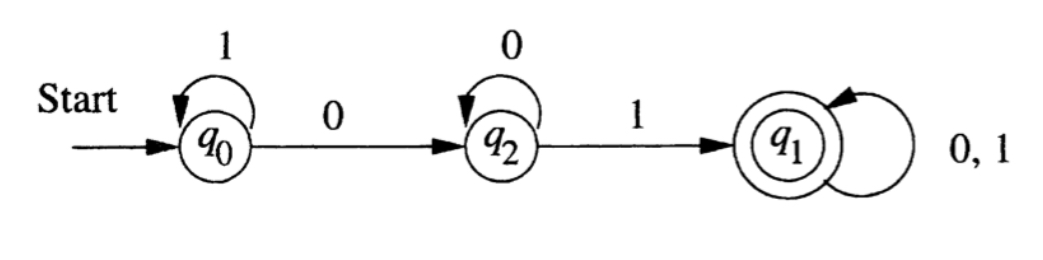
\includegraphics[width=0.5\textwidth]{dfa_diag}}
    \hspace*{.2in}
    \raisebox{-0.5\height}{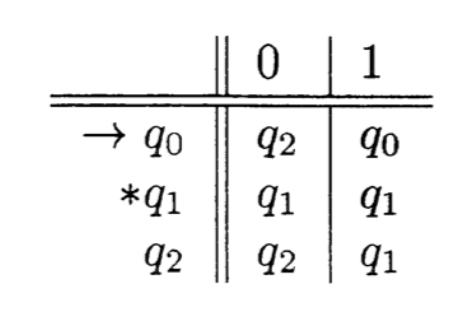
\includegraphics[width=0.25\textwidth]{dfa_table}}
    %\raisebox{-0.5\height}{\begin{tabular}{ c c c }
    %  \toprule
    %   & $0$ & $1$ \\
    %   \midrule
    %  $q_0$ & $q_2$ & $q_0$ \\
    %  $q_1$ & $q_1$ & $q_1$ \\
    %  $q_2$ & $q_2$ & $q_1$ \\
    %  \bottomrule
    %\end{tabular}}
  \end{figure}
\end{example}
To extend the transition function to strings, we define an \textbf{extended
transition function} $\hat{\delta}:Q\times \Sigma^{*}\to Q$ to describe the
state (given a starting state), after processing a sequence of input symbols.
We define by induction on the length of the input string:
\begin{enumerate}
  \item $\hat{\delta}\left( q,\epsilon \right) =q$. Starting in state $q$, if
    no inputs are read, no change in state.
  \item Suppose $w$ a string of the form $xa$, where $x\in \Sigma^{*},a\in \Sigma$,
    \[\hat{\delta}\left( q,xa \right) =\delta\left( \hat{\delta}\left( q,x \right) ,a \right).\] 
    That is, we first process all but the last symbol of $w$, then its last symbol.
\end{enumerate}
\begin{definition}[Language of a DFA]
  The \textit{language} of a DFA $A$ is denoted $L(A)$, and is defined by
  \[L(A)=\left\{ \omega | \hat{\delta}\left( q_0,\omega \right) \in F \right\},\]
  the set of strings $\omega$ that the start state $q_0$ may take to arrive at
  one of the accepting states.
\end{definition}

\subsection{Nondeterministic Finite Automata}
We now consider an automata in which we can be in several state at once.
In an NFA, it is not necessary that all states have all inputs symbols
defining a transition. In those situations, the thread of the NFA's existence
corresponding to those states simply ``dies''.
\begin{figure}[h!]
  \centering
  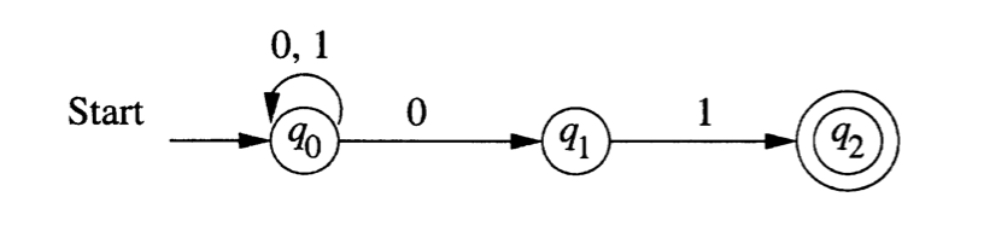
\includegraphics[width=0.5\textwidth]{nfa_diag}
\end{figure}
\begin{definition}[NFA]
  An \textit{NFA} $A = \left( Q,\Sigma,\delta,q_0,F \right) $, where:
  \begin{itemize}
    \item $Q$: A finite set of states
    \item $\Sigma$: A finite set of input symbols
    \item $\delta$: A transition function taking as argument a state and an
      input symbol and returns \textbf{a set of states}. $\delta: Q\times \Sigma\to \mathcal{P}(Q)$
    \item $q_0$: A start state, $q_0\in Q$
    \item $F$: A set of final or accepting states. $F\in \mathcal{P}\left( Q \right) $
  \end{itemize}
\end{definition}
\begin{remark}
  The only difference between an NFA and a DFA is the return type of the
  transition function.
\end{remark}
Similarly, we define the \textbf{extended transition function}
$\hat{\delta}:Q\times \Sigma^{*}\to\mathcal{P}\left( Q \right) $, the set of
states that the NFA will be in if it starts in a given state $q$ and processes
the string $\omega$. We define by induction on the length of the input string:
\begin{enumerate}
  \item $\hat{\delta}\left( q,\epsilon \right) =\left\{ q \right\}$. If no
    inputs are read, we are only in the state we began in.
  \item Suppose $w$ a string of the form $xa$, where $x\in \Sigma^{*},a\in
    \Sigma$, and that $\hat{\delta}\left( q,x \right) =\left\{ p_1,p_2,\ldots,p_k \right\}$
    \[\hat{\delta}\left( q,w \right) =\bigcup_{i=1}^{k}\delta\left( p_i,a
    \right) =\left\{ r_1,r_2,\ldots,r_m \right\}\]
    That is, we first compute $\hat{\delta}\left( q,x \right)$, then follow any
    transition from any of the possible states.
\end{enumerate}
\begin{definition}[Language of an NFA]
  The \textit{language} of an NFA $A$ is denoted $L(A)$, and is defined by
  \[L(A)=\left\{ \omega|\hat{\delta}\left( q_0,\omega \right) \cap F\neq \emptyset \right\},\]
  the set of string $\omega$ that the start state may take that does not
  definitively lead to a nonaccepting state. The set of strings such that the
  possibilities contain at least one accepting state.
\end{definition}

\subsubsection{NFAs with $\epsilon$-Transitions}
We consider an automaton in which we allow a transition on $\epsilon$. The NFA
is hence allowed to make a transition without receiving an input symbol.
\begin{figure}[h!]
  \centering
  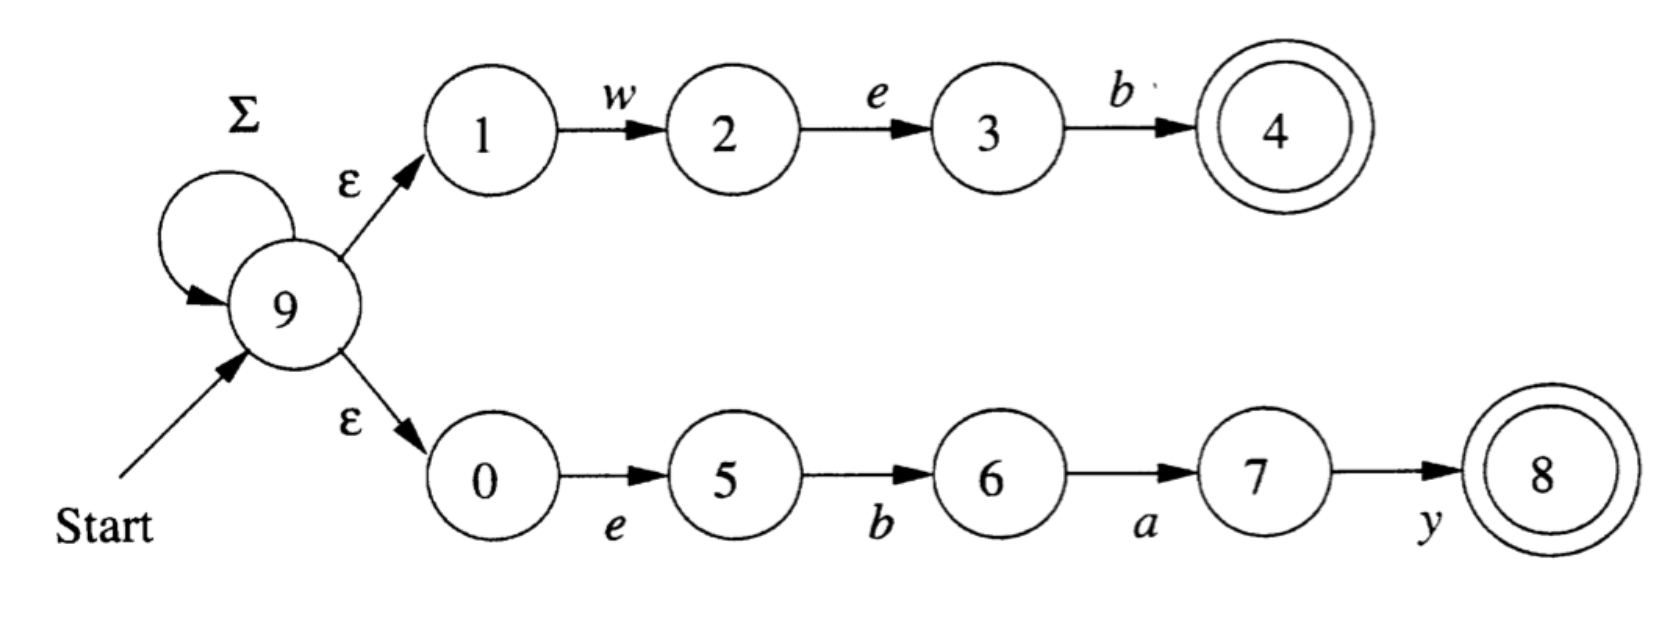
\includegraphics[width=0.5\textwidth]{nfa_epsilon_diag}
\end{figure}
\begin{definition}[$\epsilon$-NFA]
  An $\epsilon$-NFA $A=\left( Q,\Sigma,\delta,q_0,F \right) $, where:
  \begin{itemize}
    \item $Q$: A finite set of states
    \item $\Sigma$: A finite set of input symbols
    \item $\delta$: A transition function taking as argument a state and an
      input symbol (including $\epsilon$) and returns \textbf{a set of states}.
      $\delta: Q\times (\Sigma\cup \left\{ \epsilon \right\})\to \mathcal{P}(Q)$
    \item $q_0$: A start state, $q_0\in Q$
    \item $F$: A set of final or accepting states. $F\in \mathcal{P}\left( Q \right) $
  \end{itemize}
\end{definition}
To define an extended transition function for $\epsilon$-NFAs, we first define
the \textit{$\epsilon$-closure} of a state recursively:
\begin{enumerate}
  \item $q\in \epsilon$-closure$\left( q \right) $
  \item If $p\in \epsilon$-closure$\left( q \right)\wedge\delta\left( p,\epsilon \right) =r \implies r\in \epsilon$-closure$\left( q \right) $.
\end{enumerate}
The $\epsilon$-closure of a state $q$ is the set of all states reachable from
$q$ using only $\epsilon$ transitions.
We further define the $\epsilon$-closure of a set of states $S$:
\[\epsilon\text{-closure}\left( S \right) =\bigcup_{q\in S} \epsilon\text{-closure}\left( q \right).\]
We now define the \textbf{extended transition function}
$\hat{\delta}:Q\times \Sigma^{*}\to\mathcal{P}\left( Q \right) $, the set of
states that the $\epsilon$-NFA will be in if it starts in a given state $q$ and processes
the string $\omega$. We define by induction on the length of the input string:
\begin{enumerate}
  \item $\hat{\delta}\left( q,\epsilon \right) =\epsilon\text{-closure}\left(
    q \right)$.\ (by the definition of $\epsilon$-closure) \item Suppose $w$ a string of the form $xa$, where $x\in \Sigma^{*},a\in
    \Sigma$ (WLOG, $\epsilon$ not in $\Sigma$), and that $\hat{\delta}\left(
    q,x \right) =\left\{ p_1,p_2,\ldots,p_k \right\}$
    \[\hat{\delta}\left( q,w \right) =\bigcup_{i=1}^{k}\delta\left( p_i,a
    \right) =\epsilon\text{-closure}\left(   \left\{ r_1,r_2,\ldots,r_m \right\}\right)\]
    That is, we first compute $\hat{\delta}\left( q,x \right)$, then follow any
    transition from any of the possible states, then consider the possibility
    of any $\epsilon$ transitions from the possible states.
\end{enumerate}

\begin{remark}
  A $\epsilon$-NFA $E=(Q_E,\Sigma,\delta_E,q_0,F_E)$ accepts the same language
  as the DFA $D=\left( Q_D,\Sigma,\delta_D,q_D,F_D \right) $ where:
  \begin{itemize}
    \item $Q_D=\left\{ \epsilon\text{-closure}\left( S \right) | S\in
      \mathcal{P}(Q_E) \right\}$
    \item $q_D=\epsilon\text{-closure}\left( q_0 \right) $
    \item $F_D = \left\{ S| S\subseteq Q_D \wedge S\cap F_E\neq
      \emptyset\right\}$
    \item $\delta_D\left( S,a
  \right) =\epsilon\text{-closure}\left( \bigcup_{p\in S} \delta_E\left( p,a \right)  \right) $
  \end{itemize}
\end{remark}

\subsection{DFAs vs NFAs}
\subsubsection{Equivalence of DFAs and NFAs}
\begin{theorem}
  A language $L$ is accepted by some DFA if $L$ is accepted by some NFA\@.
\end{theorem}
\begin{proof}
Suppose an NFA $N=\left( Q_N,\Sigma,\delta_N,q_0,F_N \right) $. We consider the
DFA $D=\left( Q_D,\Sigma,\delta_D,\left\{ q_0 \right\} ,F_D \right) $, where
\begin{itemize}
  \item $Q_D =\mathcal{P}\left( Q_N \right) $. Intuitively, each state of the
    DFA represents a state of the entire NFA\@.
    \begin{remark}
      This conversion is known as \textit{subset construction}, involving
      constructing all subsets of the set of states of the NFA\@. Often, not all
      states are accessible from the start state. Inaccessible states can be
      discarded.
    \end{remark}
  \item $F_D = \left\{ S| S\subseteq Q_N \wedge S\cap F_N\neq
    \emptyset\right\}\subseteq \mathcal{P}(Q_N)$. That is, $F_D$ consists all
    sets of $N$'s states that include at least one accepting state of $N$.
  \item $\delta_D\left( S,a \right) =\bigcup_{p\in S} \delta_N\left( p,a
    \right) $, given $S\in \mathcal{P}\left( Q_N \right)$, and $ a\in \Sigma$.
    We consider all possible current states, and take the union of all possible
    states after processing input $a$
\end{itemize}
To prove that $\forall w\in \Sigma^{*}\left( \hat{\delta}_D\left( \left\{ q_0 \right\},\omega \right)=\hat{\delta}_N\left( q_0,w \right) \right) $, we induct on the length of $\omega$:
\begin{enumerate}
  \item \textit{Base case:} $\omega=\epsilon$
    \[\hat{\delta}_D\left( \left\{ q_0  \right\} ,\epsilon  \right)=\left\{ q_0
    \right\}=\hat{\delta}_N\left( q_0,\epsilon \right).\]
  \item \textit{Inductive step: }
    \begin{align*}
      \hat{\delta}_D\left( \left\{ q_0 \right\},\omega a\right)=&\delta_D\left(
      \hat{\delta}_D\left( \left\{ q_0 \right\},\omega \right) ,a \right)\\
        =&\bigcup_{q\in \hat{\delta}_D\left( \left\{ q_0 \right\} ,\omega\right)} \delta_N\left( q,a \right) \\
        =&\bigcup_{q\in \hat{\delta}_N\left(  q_0 ,\omega\right)} \delta_N\left( q,a \right) \\
        =&\hat{\delta}_N\left( q_0,wa \right).
    \end{align*}
\end{enumerate}
Since $\hat{\delta}_D\left( \left\{ q_0 \right\} ,\omega\right)\in F_D\iff\hat{\delta}_N\left( q_0,wa \right)\cap F_N \neq \emptyset$, we have $L(N)=L(D)$.\qed%
\end{proof}

\begin{theorem}
  A language $L$ is accepted by some DFA only if $L$ is accepted by some NFA\@.
\end{theorem}
\begin{proof}
  Intuitively, we take the transition diagram for the DFA as a transition diagram
  for an NFA, which has only one choice of transition at any state.\ \qed%
\end{proof}

Consider a language that can be described by some NFA and some DFA\@. The DFA in
practice has about as many states as the NFA, but often with more transitions.
In the worst case, however, the smallest DFA can have $2^{n}$ states while the
smallest NFA for the same language only has $n$ states.

\subsubsection{Languages of Automata}
\begin{definition}[Regular Language]
  If $L$ is $L(A)$ for some DFA $A$, then $L$ is a regular language.
\end{definition}
\begin{corollary}
  $L$ is a regular language $\iff$ $L$ is $L(N)$ for some NFA $N$.
\end{corollary}

\begin{theorem}
  Given a non-empty finite alphabet $\Sigma$, there exists a countable number of regular languages.
\end{theorem}
Since each regular language can be represented by an automaton, there exist
finite, or countably infinite regular languages. That is, there exist
languages that are not accepted by any automata and is hence non-regular.

\subsection{Minimisation of Automata}\label{minimisation}

\subsubsection{Prerequisites}
Suppose a regular language $L$. We define the equivalence relation for $u,w\in \Sigma$
\[u \equiv_L w\iff \left[ \forall x\in \Sigma, ux\in L \iff wx\in L \right].\]
We denote $equiv(w)$ the equivalence class of $w$.

\begin{definition}[Distinguishable States]
  We say that $(p,q)$ is distinguishable $\iff\exists w\in \Sigma^{*}$ such that
  \[\hat{\delta}\left( p,w \right)\in F\wedge \hat{\delta}\left( q,w \right)
  \notin F\qquad\vee\qquad\hat{\delta}\left( p,w \right)\notin F\wedge
\hat{\delta}\left( q,w \right) \in F.\] 
\end{definition}
\begin{remark}
  \[(p,q)\text{ is indistinguishable}\iff \left[ \forall w\in \Sigma^{*},
  \hat{\delta}\left( p,w \right)\notin F\iff \hat{\delta}\left( q,w \right) \in
F\right].\] 
\end{remark}

\subsubsection{Minimal DFA for $L$}
If there is a finite number of equivalence classes, $\exists$ a DFA $D=\left(
Q,\Sigma,\delta,q_0,F\right)$ where:
\begin{itemize}
  \item $Q=\left\{ equiv\left( \omega \right) | \omega\in \Sigma^{*} \right\}=\Sigma^{*}/\equiv_L$
  \item $\delta:(\Sigma^{*}/\equiv_L \times \Sigma)\to \Sigma^{*}/\equiv_L$ defined
    $\delta\left( equiv(\omega),a \right) =equiv(wa)$
  \item $q_0=equiv(\epsilon)$
  \item $F=\left\{ equiv(\omega) | w\in L \right\}$
\end{itemize}
which, by definition of the equivalence relation, accepts $L$. It is also the
minimal DFA for $L$.

\begin{lemma}
  $u \not\equiv_L \omega\implies \hat{\delta}'\left( q_0',u \right) \neq
  \hat{\delta}'\left( q_0',w \right) $.
\end{lemma}
\begin{proof}
  Suppose not. That is $u\not \equiv_L
  w\wedge\hat{\delta}'\left( q_0',u \right) = \hat{\delta}'\left( q_0',w
  \right)$. Then $\exists x\in \Sigma^{*}$ such that WLOG, $ux\in L\wedge
  wx\notin L$. But $\hat{\delta}'\left( q_0',u \right) = \hat{\delta}'\left(
  q_0',w \right)$ and $A'$ accepts either both or neither. Hence a
  contradiction.\qed%
\end{proof}

\begin{prop}
  $D$ is minimal.
\end{prop}
\begin{proof}
  Suppose a DFA $A'=\left( Q',\Sigma,\delta',q_0',F' \right) $ also accepting
  $L$. From the lemma, we have
  \[u \not\equiv_L \omega\implies \hat{\delta}'\left( q_0',u \right) \neq
  \hat{\delta}'\left( q_0',w \right).\]
  Let $u\equiv_{A'}w\iff\hat{\delta}'\left( q_0',u \right) =
  \hat{\delta}'\left( q_0',w \right)$. Then $u\equiv_L \implies u\equiv_{A'}
  w$. Hence $\equiv_{A'}$ divides the equivalence classes of $\equiv_{L}$ into
  finer equivalence classes, and $\equiv_L$ is minimal.\qed%
\end{proof}

\subsubsection{Minimal DFA Construction Algorithm}
Suppose we are given a DFA $A=\left( Q,\Sigma,\delta,q_0,F \right) $.
We determine all distinguishable pairs with the following recursive algorithm:
\begin{enumerate}
  \item \textit{Base case:} Each pair $(p,q)$ such that $p\in F$ and $q\notin
    F$ (or vice versa) is distinguishable.
  \item \textit{Inductive step:} If $\exists a\in \Sigma\left[  \delta\left(
    p,a \right) \text{ and }\delta\left( q,a \right) \text{ are
  distinguishable} \right]$, then $(p,q)$
    is distinguishable.
  \item Steps 1 and 2 are repeated until no more pairs can be added.
  \item The remaining pairs are non-distinguishable states.
\end{enumerate}
To compute the distinguishable states, we utilise the table-filling algorithm:
\begin{figure}[h!]
  \centering
  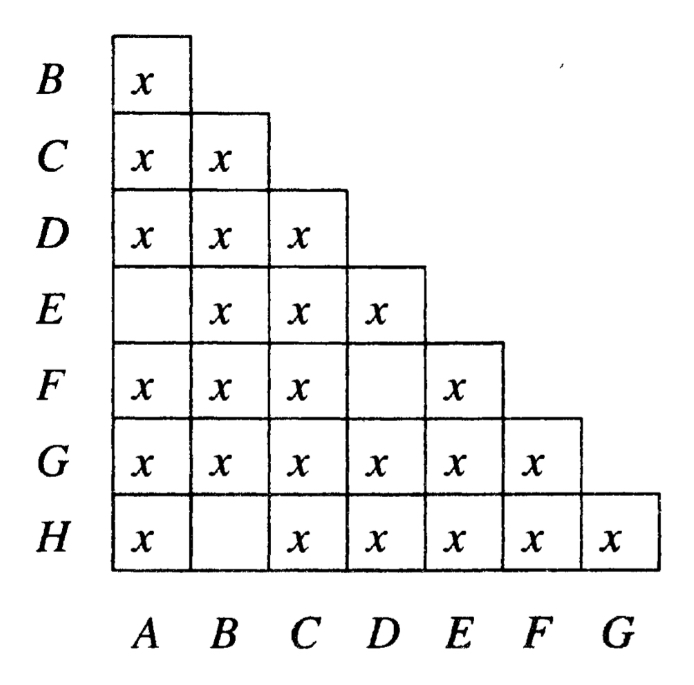
\includegraphics[width=0.3\textwidth]{table_filling}
\end{figure}
We then form the new DFA as follows:
\begin{enumerate}
  \item Remove all unreachable states.
  \item Find all nondistinguishable pairs of states using the algorithm. They
    are equivalent. This yields an equivalence relation
  \item Form the new DFA with:
    \begin{itemize}
      \item $Q_{new}$ as the set of the equivalence classes.
      \item The same $\Sigma$
      \item The transitions from each equivalence class is based on the
        corresponding transition in the original DFA\@:
        \[\delta\left( p,a \right) =q \implies\delta_{new}\left( E_p,a \right)=E_q.\]
        where $E_p, E_q$ are the equivalence classes of $p,q$ respectively.
      \item $q_{0,new}=equiv(q_0)$
      \item $F_{new}=\left\{ equiv(\omega) | w\in F \right\}$
    \end{itemize}
\end{enumerate}
% TODO: Add proof of correctness of table-filling algorithm
% TODO: Add proof of correctness of new DFA

\subsection{Parallel Simulation of n-DFAs}
Suppose two DFAs $A=\left(Q,\Sigma,\delta,q_0,F\right)$ and $A'=\left( Q',\Sigma,
\delta',q_0',F' \right) $.
We may construct another DFA $A''=\left( Q\times
Q',\Sigma,\delta'',\left(q_0,q_0'\right),F'' \right) $, where
\[\delta''\left( \left( q,q' \right) ,a \right) =\left( \delta\left( q,a
\right) ,\delta'\left( q',a \right)  \right).\] 
and $F''$ depends on need.
\begin{example}[Definitions of $F''$]\ 
   \begin{itemize}
    \item $F''=F\times F'$ finds the intersections of the two automata.
    \item $F''=F\times Q'\cup Q\times F'$ finds the union of the two automata.
  \end{itemize}
\end{example}
This simulates the two DFAs in parallel.
\begin{remark}
  By repeated application, we may simulate any boolean combination of
  automata.
\end{remark}


\subsection{Regular Expressions}
Through regular expressions, another type of language-defining notation that
algebraically describes a language, we are able to declaratively express the
strings we want to accept. Each regular expression denotes a (regular) language.
\subsubsection{Operators}
Given a regular expression $E$, we denote $L(E)$ for the language that $E$
denotes. We then define regular expressions inductively (with various
operators), as follows:
\begin{enumerate}
  \item \textit{Basis Step:}
    \begin{itemize}
      \item Constant $\epsilon$ is a regular expression, with
        $L(\epsilon)=\left\{ \epsilon \right\}$.
      \item Constant $\emptyset$ is a regular expression, with $L(\emptyset)=\emptyset$.
      \item If $a\in \Sigma$, $a$ is a regular expression, with $L(a)=\left\{ a
        \right\}$.
    \end{itemize}
  \item \textit{Inductive Step:} Given regular expressions $E$ and $F$,
    \begin{itemize}
      \item $E+F$ is a regular expression denoting union, $L(E+F)=L(E)\cup L(F)$.
      \item $EF$ is a regular expression denoting concatenation, $L(EF)=L(E)L(F)$.
      \item  $E^{*}$ is a regular expression denoting its (Kleene's) closure,
        $L(E^{*})={\left( L\left( E \right)  \right)}^{*}$
      \item $E^{+}$ is a regular expression denoting its closure, without $\epsilon$, $L(E^{+})=EE^{*}$
      \item $(E)$ is a regular expression denoting the same language, $L\left( \left( E \right)  \right) =L(E)$
    \end{itemize}
\end{enumerate}
We further define the order of precedence of the operators:
 \begin{enumerate}
  \item The parantheses operator is of highest precedence, to specify the
    desired grouping of regular expressions.
  \item The star operator is of highest precedence, applied to the smallest
    sequence of symbols to its left that is a well-formed regular expression.
  \item The concatenation operator groups all expressions that are
    \textit{juxtaposed} (adjacent without intervening operators). Concatenation is associative.
  \item The union binary operator groups its operands. Union is associative.
\end{enumerate}

\subsubsection{Converting Automaton to Regular Expression}
\begin{theorem}  
  If $L = L(A)$ for some DFA $A$, then there is a regular expression $R$ such
  that $L=L(R)$. That is, every regular language can be defined by a regular
  expression.
\end{theorem}
\begin{proof}
  Suppose a DFA $A=\left( Q,\Sigma,\delta,q_{start},F \right)$. Without loss of generality, suppose
  $Q=\left\{ 1,2,\ldots,n \right\}$ for some $n$ and $q_{start}=1$.
  Let $R^{k}_{i,j}$ denote the regular expression for the set of strings which
  can be formed by going from state $i$ to state $j$ only using intermediate
  states $\le k$. We have
  \[L(A)=L\left(\sum_{j\in F} R_{1,j}^{n}\right)\]
  We compute by induction:
  \begin{enumerate}
    \item \textit{Base step:} $R_{i,j}^{0}$. That is, the path must have no
      intermediate states at all. We only have an arc from (state) $i$ to $j$,
      or a path of length 0 consisting only $i$.\\
      \[i\neq j \implies R_{i,j}^{0}=a_1+a_2+\cdots+a_m, \qquad\forall a_r\in \Sigma, \delta\left( i,a_r \right) =j.\] 
      \[i=j \implies R_{i,i}^{0}=\epsilon+a_1+a_2+\cdots+a_m, \qquad\forall a_r\in \Sigma, \delta\left( i,a_r \right) =i.\] 
    \item \textit{Inductive step:} Suppose there is a path from state $i$ to
      $j$ going through states no higher than $k$.
      \[R_{i,j}^{k+1}=R_{i,j}^{k}+R_{i,k+1}^{k}{\left(R_{k+1,k+1}^{k}\right)}^{*}R_{k+1,j}^{k}.\] 
      We then have the case where the path does not go through state $k+1$ at
      all, and the case where it goes through $k+1$ at least once.
  \end{enumerate}
  \begin{figure}[h!]
    \centering
    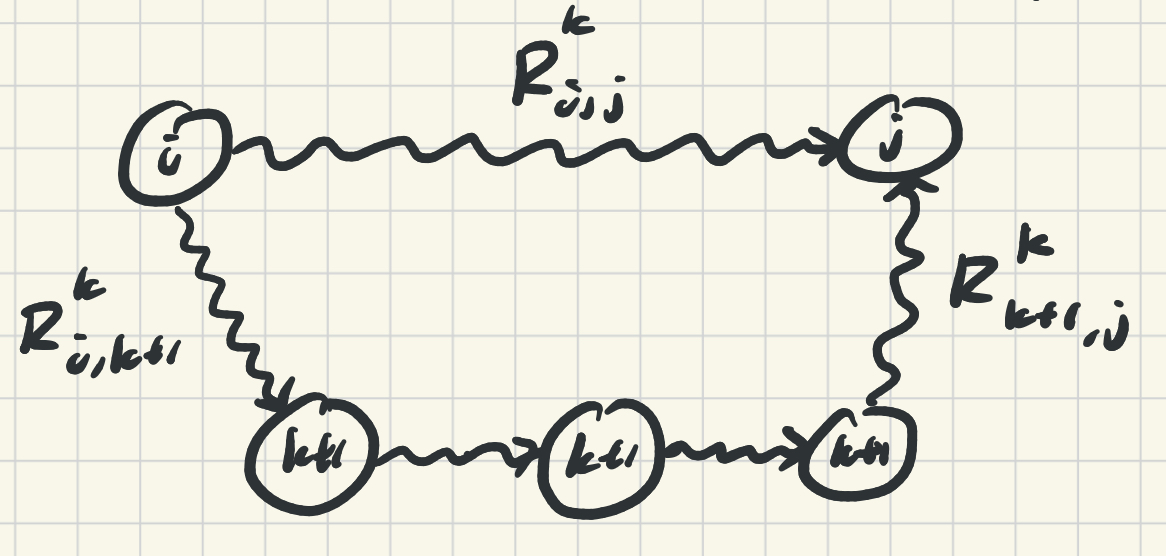
\includegraphics[width=0.5\textwidth]{automata_regex}
  \end{figure}
  We may then obtain
  $L(A)=L\left(\sum_{j\in F} R_{1,j}^{n}\right)$.\qed%
\end{proof}
\begin{remark}
  The construction of a regular expression from automata could be applied to
  NFA or $\epsilon$-NFA, but we construct about $n^{3}$ expressions, with
  each's length growing by a factor of 4 each inductive step, resulting in a
  expression on the order of $4^{n}$ symbols for an $n$-state automaton.
\end{remark}
% TODO: Add Converting DFA's to Regular Expressions by Eliminating States TB pg. 98

\subsubsection{Converting Regular Expression to Automaton}
\begin{theorem}
  Every language defined by a regular expression can be defined by an automaton.
\end{theorem}
We may construct an automaton through structural induction on the expression,
constructing automata for the basis expressions and combining them into
larger automata that fits the various operators.

\begin{proof}
  Suppose $L=L(R)$for a regular expression $R$. We construct a $e$-NFA $E$ with:
  \begin{enumerate}
    \item Exactly one accepting state.
    \item No transition into the starting state.
    \item No transition out of the accepting state.
    \item Starting state $\neq$ Accepting state.
  \end{enumerate}
  For the bases, we create automata that accepts the languages 
  \begin{itemize}
    \item (a) $L(\epsilon)$,
    \item (b) $L(\emptyset)$,
    \item (c) $L(a)$
  \end{itemize}
  We then assume that we have the automaton for the immediate subexpressions of
  a given regular expression. We then have the four cases: 
  \begin{itemize}
    \item (a) $R+S$,
    \item (b) $RS$,
    \item (c) $R^{*}$
    \item $R^{+}$ which is constructed from the automaton of $R^{*}$, but
      without the $\epsilon$ transition from the starting to the accepting
      state
    \item $(R)$ where the automaton does not change.
  \end{itemize}
  \begin{figure}[h!]
    \centering
    \raisebox{-0.5\height}{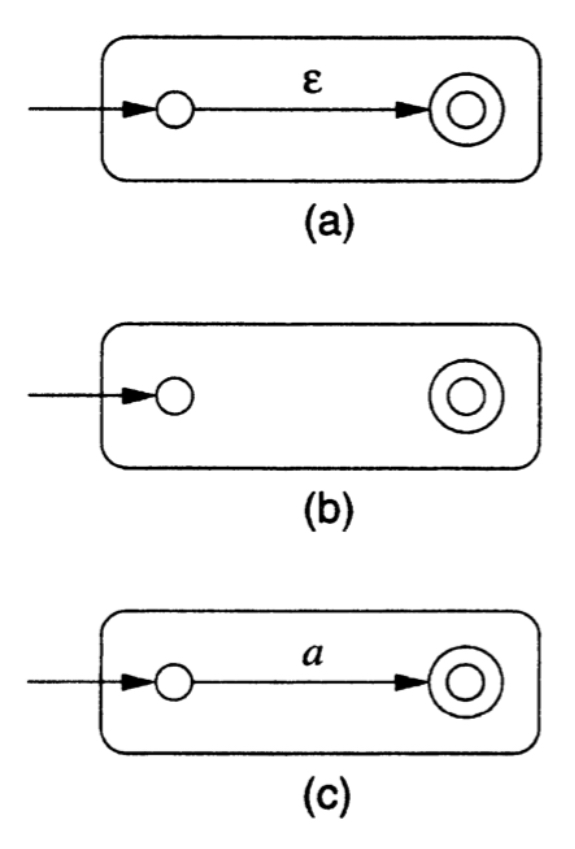
\includegraphics[width=0.2\textwidth]{regex_automata}}
    \hspace*{.2in}
    \raisebox{-0.5\height}{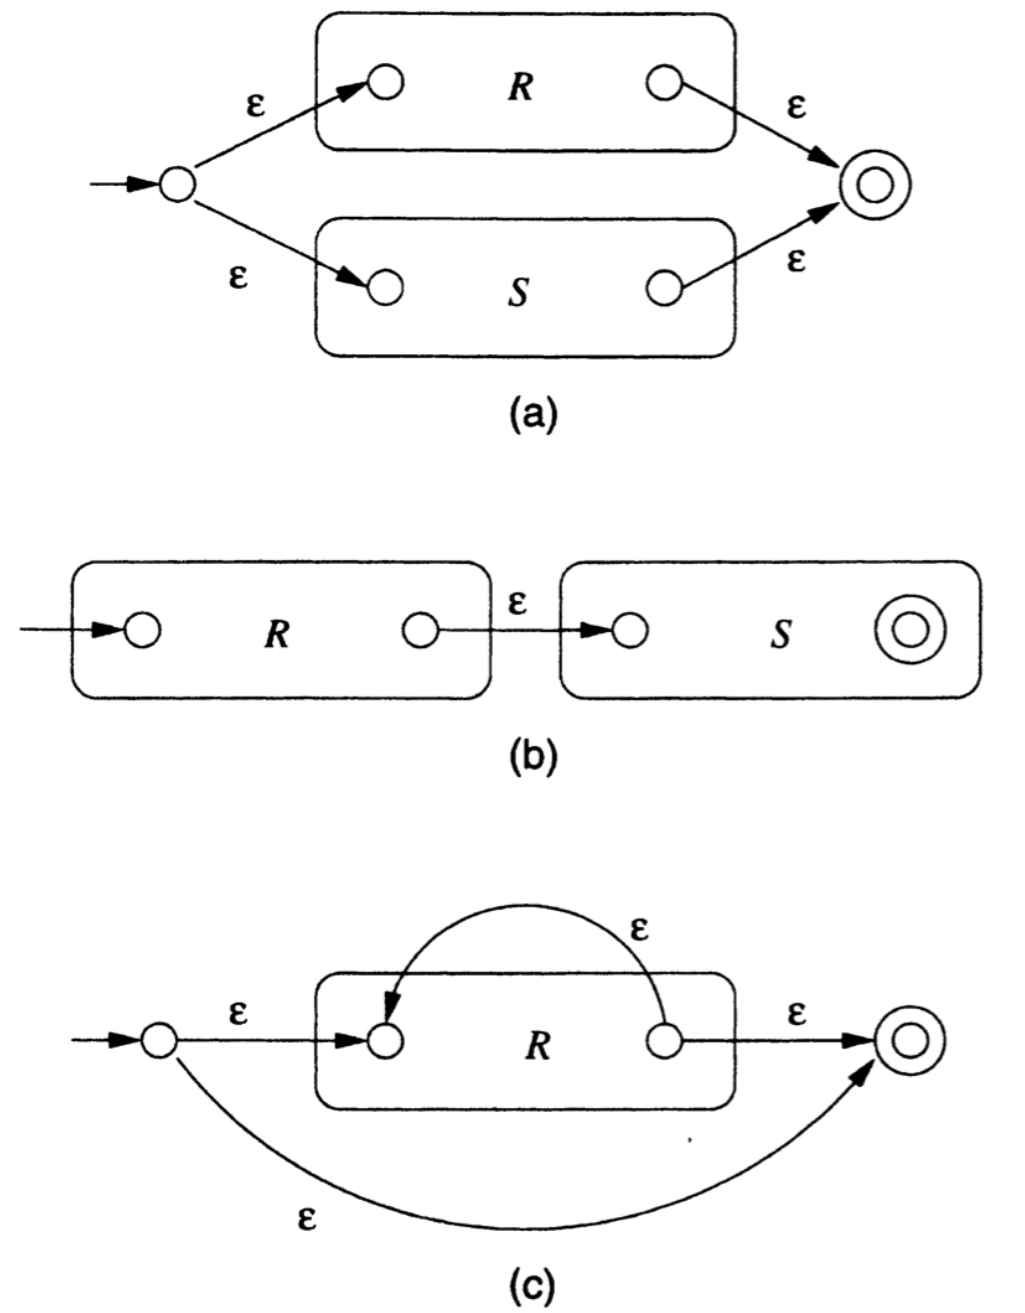
\includegraphics[width=0.35\textwidth]{regex_automata_2}}
  \end{figure}
  The constructed automata satisfy the four conditions, providing the language
  of the regular expression.\qed%
\end{proof}

\subsubsection{Algebra of Regular Expressions}
We find various useful results for simplifying regular expressions and to keep
the size of expressions manageable. We consider the algebra of regular
expressions, analysing properties such as associativity, commutativity and
distributivity, as well as relevant identities and annihilators. For regular
expressions $L, M, N$:
\paragraph{Associativity, Commutativity and Distributivity}
\begin{itemize}
  \item $L+M=M+L$: Commutative law for union.
  \item  $(L+M)+N=L+(M+N)$: Associative law for union. With the commutative
    law, we may take union in any order.
  \item $(LM)N=L(MN)$: Associative law for concatenation. Concatenation is non-commutative.
  \item $L(M+N)=LM+LN$: Left-distributive law of concatenation over union.
  \item $(M+N)L=ML+NL$: Right-distributive law of concatenation over union.
\end{itemize}
\paragraph{Identities, Annihilators and Idempotence}
\begin{itemize}
  \item $\emptyset+L=L+\emptyset=L$: $\emptyset $ identity for union.
  \item $\epsilon L = L \epsilon=L$: $\epsilon$ identity for concatenation.
  \item $\emptyset L=L\emptyset =\emptyset $: $\emptyset $ annihilator for concatenation.
  \item $L + L = L$: Idempotence law for union.
\end{itemize}
\paragraph{Closures}
\begin{itemize}
  \item ${\left( L^{*} \right)} ^{*}=L^{*}$: Closing an expression that is
    already closed does not change.
  \item $\emptyset ^{*}=\epsilon$
  \item $\epsilon^{*}=\epsilon$ 
  \item $L^{+}=LL^{*}=L^{*}L$ 
  \item $L^{*}=L^{+}+\epsilon$
  \item ${(L+M)}^{*}={(L^{*}M^{*})}^{*}$
\end{itemize}

\subsection{Regular Languages}
To show that a given language is nonregular, we may use the pumping lemma.
Intuitively, we can always find a nonempty string $y$ not too far from the
beginning that can be repeated any number of times, or deleted while keeping
the resulting string in $L$.
\begin{lemma}
  Let $L$ be a regular language. Then $\exists n=f(L)$ such that $\forall\omega\in L$,
  $\left| \omega \right| \ge n$, $\exists x,y,z\in \Sigma^{*},\omega=xyz$ such that:
  \begin{itemize}
    \item $\left| xy \right| \le n$. That is, string to be pumped is not too
      far from the start of the string.
    \item $y\neq\epsilon$. The string to be ``pumped'' cannot be empty.
    \item $\forall i\ge 0$, $xy^{k}z\in L$
  \end{itemize}
\end{lemma}
The contrapositive of the lemma is used to prove that a language is
nonregular. That is, $\forall n\in \mathbb{N}$, $\exists w\in L$, such that
$\left| \omega \right| \ge n$, $\forall x,y,z\in \Sigma^{*}$, where $\omega=xyz$,
$\left| xy \right| \le n$, $y\neq\epsilon$, we have
\[\exists i\in \mathbb{N}\left( xy^{i}z\notin L \right)\]
\begin{proof}
  Suppose $L$ is regular. Then $\exists$ DFA $A=\left( Q, \Sigma, \delta, q_0,F
  \right)$ such that $L=L(A)$. Suppose $\left| Q \right|=n$. Consider a string
  $\omega\in \Sigma^{*},\left| w \right| \ge n$. Then $w=a_1a_2\cdots a_m$ for
  some $m\ge n, a_i\in \Sigma$. For $i=0,1,\ldots,n, p_i:=\hat{\delta}\left(
  q_0,a_1a_2\cdots a_i \right)$. $p_i$ is the state of $A$ after reading the
  first $i$ symbols of $\omega$.\\
  Since there are $n$ different states and $n+1$ different $p_i$'s, by the
  pigeonhole principle, $\exists 0\le i<j<n$ such that $p_i=p_j$. Let:
  \begin{itemize}
    \item $x=a_1a_2\cdots a_i$ 
    \item $y=a_{i+1}a_{i+2}\cdots a_j$
    \item $z=a_{j+1}a_{j+2}\cdots a_m$
  \end{itemize}
  By processing $x$, $A$ takes up state $p_i$, after which $y$ takes it from
  $p_i$ back to $p_i$, and $z$ is the balance of $\omega$. $x=\epsilon\iff
  i=0$, and $z=\epsilon\iff j=n=m$. However, $y$ cannot be empty, since $i<j$.
  \begin{figure}[h!]
    \centering
    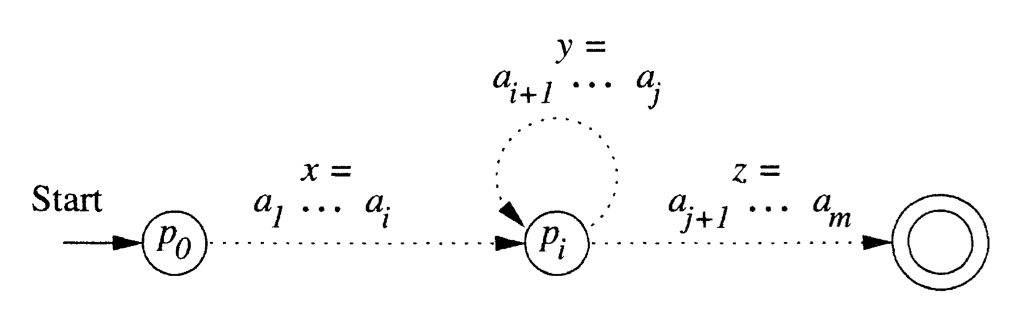
\includegraphics[width=0.5\textwidth]{rl_pumping_lemma}
  \end{figure}
  Then consider for any $k\in \mathbb{N}$, the string $xy^{k}z$:
  \begin{itemize}
    \item If $k=0$, the automaton goes from $q_0=p_0$ to $p_i=p_j$ on input
      $x$, and then from $p_i=p_j$ to the accepting state on input $z$. $A$
      accepts $xz$.
    \item If  $k>0$, the automaton goes from $q_0$ to $p_i$ on input $x$, and
      then circles $p_i$ to $p_i$ $k$ times on input $y^{k}$, and then to the
      accepting state on input $z$. $A$ accepts $xy^{k}z$.
  \end{itemize}\vspace{-7mm}\qed%
\end{proof}

By using the pumping lemma, we can construct a proof of the following structure
to show a specified language is non-regular:
\begin{prop}
  $L=\left\{ a^{m}b^{m}|m\ge 1 \right\}$ is nonregular.
\end{prop}
\begin{proof}
  Suppose $L$ is regular. Let $n$ be as in the Pumping Lemma. Let
  $\omega=a^{n}b^{n}$. Let $\omega=xyz$ as in the pumping lemma. Then $y$
  consists of only $a$'s, and $\left| y \right| >0$, $y={\left\{ a
  \right\}}^{+}$. By the pumping lemma, $xy^{2}z\in L$. But $xy^{2}z$ contains
  more $a$'s than $b$'s, and $xy^{2}z\notin L$. Hence $L$ is nonregular.
\end{proof}
\begin{prop}
  $L=\left\{ a^{p}|p\text{ is prime} \right\}$ is nonregular.
\end{prop}
\begin{proof}
  Suppose $L$ is regular. Let $n$ be as in the Pumping Lemma. Let
  $\omega=a^{p}$, where $p$ is prime and $p>n$. Let $\omega=xyz$ as in the
  pumping lemma. By the pumping lemma, $\forall k\in \mathbb{N}, xy^{k}z\in L$. Consider
  $k=p+1$. Then $xy^{k}z=a^{r}$ where 
  \[r=\left| x \right| +\left| z \right| +\left( p+1 \right) \left| y \right| =p+p\left| y \right|  \]
  and $r$ is non-prime,  and $xy^{p+1}z\notin L$. Hence $L$ is nonregular.
\end{proof}
\begin{prop}
  $L= \left\{a^i b^j | i < j\right\}$ is nonregular.
\end{prop}

\subsubsection{Closure of Regular Languages}
We have certain operations such that, when applied to the languages, the
resulting related language is also regular.

\begin{definition}[Homomorphism]
  Suppose two alphabets $\Sigma$ and $\Gamma$. Consider a mapping
  $h:\Sigma\to\Gamma^{*}$. We further define $h:\Sigma^{*}\to\Gamma^{*}$ by
  principle of induction:
  \begin{enumerate}
    \item \textit{Base case:}
      $h(\epsilon)=\epsilon$
    \item \textit{Inductive Step:}
      $h(a\omega)=h(a)\cdot h(\omega), \forall a\in \Sigma,\omega\in \Sigma^{*}$ 
  \end{enumerate}
  $h$ is called a \textit{homomorphism}. Intuitively, a homomorphism maps each
  symbol to another symbol in every string of the language.
\end{definition}

Given regular languages $L, L_1,L_2$:
\begin{itemize}
  \item $L_1\cup L_2$ is regular.
  \item $L_1\cdot L_2$ is regular.
  \item $\bar{L}=\Sigma^{*}-L$ is regular.
  \item $L_1\cap L_2$ is regular.
  \item $L_1-L_2$ is regular.
  \item $L^{R}$ is regular.
  \item $h(L)$ is regular, for some homomorphism $h$.
\end{itemize}
We may prove the results by constructing a regular expression through principle
of induction on its length, from the base cases of a regular expression
$\emptyset,\epsilon,a\in \Sigma$ and the defined operations.
\begin{remark}
  Supposing $L$ is a regular language over an alphabet $\Sigma_1$. Then $L$ is also a regular language
  over an alphabet $\Sigma_2\supseteq\Sigma_1$, by considering the same DFA over $\Sigma_2$.
\end{remark}

\subsubsection{Decision Problems of Regular Languages}
We may examine some properties of regular languages through conversion between
the equivalent forms of representing regular languages.\\

\begin{figure}[h!]
  \centering
  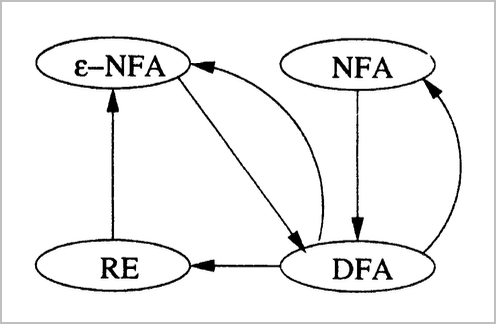
\includegraphics[width=0.3\textwidth]{conversions}
\end{figure}

We check the \textbf{emptiness of regular languages} by considering the automaton, and
checking whether any accepting states are reachable from the starting state. That is,
\[L=\emptyset \iff \forall q\in F, q\text{ is unreachable}.\] 
We compute this using a recursive algorithm:
\begin{itemize}
  \item \textit{Base case:} The start state is reachable from the start state.
  \item \textit{Inductive step:} If $p$ is reachable from the start state, all
    states $q$ such that $\exists a\in \Sigma, \delta(p,a)=q$ are reachable
    from the start state.
\end{itemize}

We check for \textbf{membership} by converting whichever representation available into a
DFA, and then simulating the DFA\@. Alternatively, if given another automaton, we
may attempt to simulate the NFA or $\epsilon$-NFA itself, keeping track of all
possible states.\\

\textbf{Two automata $A, A'$ are equivalent} $\iff$ the minimisation of $A$ is the same
as the minimisation of $A'$, except for renaming of the states. (Minimisation
of DFA, Subsection~\ref{minimisation})

\subsection{Linear Grammars}
\begin{definition}[Right Linear Grammar]
  A \textbf{Right Linear Grammar} is a CFG where all productions are of the form:
  \begin{align*}
  A\to\omega\beta\qquad &\omega\in T^{*},\quad \beta\in V\\
  A\to \omega\qquad&\omega\in T^{*}
  \end{align*}
  Similarly, a \textbf{Left Linear Grammar} is one in which all productions are of the form:
  \begin{align*}
  A\to\beta\omega\qquad &\omega\in T^{*},\quad \beta\in V\\
  A\to \omega\qquad&\omega\in T^{*}
  \end{align*}
\end{definition}
\begin{theorem}
  Every regular language can be generated by a right-linear grmmar.
\end{theorem}
\begin{proof}
  Suppose a regular language $L$. There exists a DFA $A=\left( Q,\Sigma,\delta,q_0,F \right) $ such
  that $L(A)=L$. WLOG, assume that $Q\cap \Sigma=\emptyset$. Consider the
  right-linear grammar $G=\left( Q,\Sigma,P,q_0 \right) $, where:
  \begin{enumerate}
    \item $\forall q,p\in Q,a\in \Sigma$
      \[\delta\left( q,a \right) =p\iff\exists\text{ a production }(q\to ap)\in P.\] 
    \item $\forall q\in F$
      \[\exists \text{ a production }(q\to\epsilon)\in P.\]
  \end{enumerate}
  We induct on the length $\left| \omega \right| $ to show that
  $\hat{\delta}\left( q_0,\omega \right)=p\iff q_0 \Rightarrow _G^{*}\omega p$.
  \begin{enumerate}
    \item \textit{Basis Step}: For $\left| \omega \right| =0$, $\omega=\epsilon$ and 
      \[\hat{\delta}\left( q_0,\omega \right)=p\iff p=q_0\iff q_0 \Rightarrow _G^{*}\omega p\]
    \item \textit{Inductive Step}: Consider $\omega=ua$, for some $a\in \Sigma$
      and $u\in \Sigma_{\le k}$. We have:
      \begin{align*}
        \hat{\delta}\left( q_0,ua \right) =p'\iff&\exists p\in Q,\quad
        \hat{\delta}\left( q_0,u \right) =p\wedge\delta\left( p,a \right) =p'\\
        \iff&\exists p\in Q,\quad q_0 \Rightarrow _G^{*}up\wedge p\to ap'\\
        \iff&q_0 \Rightarrow _G^{*}uap'=\omega p'
      \end{align*}\vspace{-4mm}\qed%
  \end{enumerate}
\end{proof}
\vspace{-4mm}
\begin{theorem}
  A language generated by a right-linear grammar is regular.
\end{theorem}
\begin{proof}
  Suppose a right-linear grammar $G=\left( V,\Sigma,P,S \right)$. WLOG, suppose
  $V\cap \Sigma=\emptyset$ and each productions are of the form $A\to bC$ or $A\to\epsilon$ where
  $A,C\in V$ and $b\in \Sigma\cup \left\{ \epsilon \right\} $. Consider the
  NFA $A=\left( V,\Sigma,\delta,S,F \right) $, where:
  \[\left( A\to aB \right)\in P\iff B\in \delta\left( A,a \right).\]
  and $F =\left\{ A\in V|(A\to\epsilon)\in P \right\} $
  We induct on the length $\left| \omega \right| $ to show that $A \Rightarrow _G^{*}\omega B\iff B\in \hat{\delta}\left( A,\omega \right) $.
  \begin{enumerate}
    \item \textit{Basis Step}: For $\left| \omega \right| =0$, $\omega=\epsilon$ and
      \[A \Rightarrow _G^{*}B\iff A=B \iff B\in \hat{\delta}\left( A,\epsilon \right).\]
    \item Consider $\omega=ua$. Then
      \begin{align*}
        A \Rightarrow _G^{*} \omega B=uaB\iff&\exists C\in V,\quad A\Rightarrow _G^{*}uC\wedge C\Rightarrow _G aB\\
        \iff&\exists C\in V,\quad\hat{\delta}\left( A,u \right) =C\wedge \delta\left( C,a \right) =B\\
        \iff&\hat{\delta}\left( A,ua \right)=\hat{\delta}\left( A,\omega \right)  =B
      \end{align*}\vspace{-4mm}\qed%
  \end{enumerate} 
\end{proof}



\section{Context Free Languages}
We now consider a larger class of languages known as the \textbf{context-free
languages}. These languages can be defined by a recursive notation known as
\textit{context-free grammars}, or a automaton-like notation known as
\textit{pushdown automaton}.\\

Intuitively, the class of CFLs comprises the RLs, and languages in which
symmetry is required, and certain forms of matching (in opposite directions).

\subsection{Context-Free Grammars}
\begin{definition}[CFG]
  A \textit{CFG} $C=\left( V,T,P,S \right) $, where:
  \begin{itemize}
    \item $V$: A finite set of non-terminals
    \item $T$: A finite set of terminals
    \item $P$: A finite set of productions
    \item $S$: A start symbol, $S\in V$
  \end{itemize}
  A production is of the form $A\to\gamma$, where $A\in V\wedge \gamma\in
  {\left( V\cup T \right)} ^{*}$. If we have the productions
  of $A$ $A\to\alpha_1,A\to\alpha_2,\ldots,A\to\alpha_{n}$, we may write
  $A\to\alpha_1|\alpha_2|\ldots|\alpha_{n}$
\end{definition}
\begin{example}[$L(0^{*}1{(0+1)}^{*})$]
  To generate the regular language $L(0^{*}1{(0+1)}^{*})$, consider the CFG $G=\left(
  \left\{ S,A,B \right\},\left\{ 0,1 \right\},P,S \right) $, where $P$
  comprises the productions:
  \[S\to AB,\qquad A\to 0A|\epsilon,\qquad B\to 0B|1B|\epsilon.\] 
\end{example}
\subsubsection{Derivations}
To infer if a certain string is in the language of the CFG, we may apply
\textit{recursive inference} or \textit{derivation}.
\begin{definition}[Recursive Inference]
  We may construct the string recursively from body to head. For example, given
  a production $A\to BC$, we take strings $b\in L(B)$ and $c\in L(C)$ and
  concatenate them in the proper order and infer that the resulting string is
  in $L(A)$.

  \centering
\begin{tabular}{ccccc}
   \toprule
   & String Inferred & In language of & Production used & String(s) used \\
   \midrule
  (i) & $\epsilon$ & $A$ & $A\to\epsilon$ & -- \\
  (ii) & $\epsilon$ & $B$ & $B\to\epsilon$ & -- \\
  (iii) & $0$ & $A$ & $A\to 0A$ & (i) \\
  (iv) & $0$ & $B$ & $B\to 0B$ & (ii) \\
  (v) & $1$ & $B$ & $B\to 1B$ & (ii) \\
  (vi) & $00$ & $A$ & $A\to 0A$ & (iii) \\
  (vii) & $10$ & $B$ & $B\to 1B$ & (iv) \\
  (viii) & $11$ & $B$ & $B\to 1B$ & (v) \\
  (ix) & $11$ & $S$ & $S\to AB$ & (i), (viii) \\
  \vdots & \vdots & \vdots & \vdots & \vdots\\
  \bottomrule
\end{tabular}

\raggedright
\vspace{2mm}
This procedure is known as \textbf{recursive inference}.
\end{definition}

\begin{notation}[$\Rightarrow$] 
  If $A\in V$ such that $A\to \gamma$ is a production of CFG $G$, we denote
  \[\alpha A\beta\Rightarrow_G \alpha\gamma\beta\qquad\forall\alpha,\beta\in
  {\left( V\cup T \right)}^{*}.\]
\end{notation}
\begin{definition}[Derivation]
  We can expand $S$ with one of its productions, and recursively expand each
  non-terminal with the body of its productions until a string of terminals is derived.
  \[S\Rightarrow AB \Rightarrow A1B \Rightarrow A11B \Rightarrow A110B \Rightarrow A110
  \Rightarrow 0A110 \Rightarrow 0110\]
  This is referred to as a \textbf{derivation} of $0110$. We may then define a
  derivation relation $\Rightarrow ^{*}_G$:
  \begin{enumerate}
    \item \textit{Base Case}: $\alpha \Rightarrow _G^{*} \alpha$
    \item \textit{Inductive Step}: If $\alpha \Rightarrow
      _G^{*}\beta\wedge\beta \Rightarrow _G \gamma$, then $\alpha
      \Rightarrow _G^{*}\gamma$.
  \end{enumerate}
  That is, there exists a derivation from $\alpha$ to $\beta$.
\end{definition}

\begin{definition}[Left/Right-most Derivations]
  A \textbf{leftmost derivation} is one in which at each step, the leftmost
  variable is replaced by one of its production bodies. This restricts the
  number of choices we have in deriving a string. Similarly, we can also
  have a \textbf{rightmost derivation}.
\end{definition}

\begin{definition}[Sentential Forms]
  Any string $\alpha\in {\left( V\cup T \right) }^{*}$ such that $S \Rightarrow
  ^{*}\alpha$ is called a \textbf{sentential form}, a string (of terminals or
  non-terminals) derived from the start symbol. We further have the
  analogue for left/right-most derivations, known as a
  \textit{left/right-sentential form}.
\end{definition}

\subsubsection{Parse Trees}
\begin{definition}[Parse Tree]
  We use a tree representation for derivations, where each interior node is
  labelled by a nonterminal in $V$, each leaf is labelled by a symbol in $V\cup
  T$, or $\epsilon$, and the children $X_1,X_2,\ldots,X_k$ (from the left) of
  an interior node $A$ forms the body of the production $(A\to X_1X_2\cdots
  X_k)\in P$. This is known as the \textbf{parse tree}.
  \begin{figure}[h!]
    \centering
    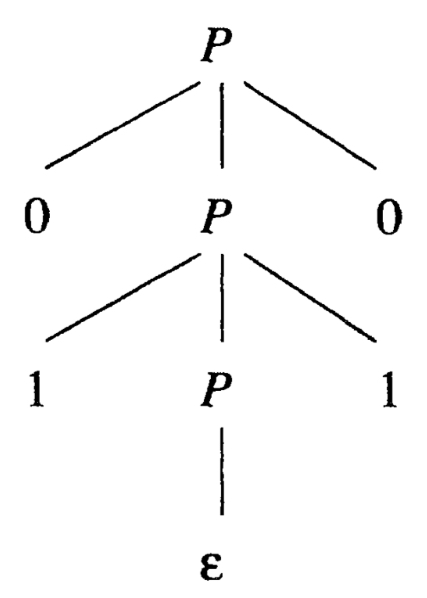
\includegraphics[width=0.17\textwidth]{parse_tree.jpeg}
  \end{figure}
  We call the in-order traversal of its leaves the \textbf{yield} of the parse
  tree.
\end{definition}
Consider the parse trees whose yields are terminal strings, and the root is
labelled by the start symbol. Then the yield is a string in the language of the
grammar.
\begin{remark}
  Derivations are non unique, but parse trees and its equivalent left-most
  derivations, right-most derivations are unique for unambiguous grammars.
\end{remark}

\subsubsection{Language of a CFG}
\begin{definition}[Language of a CFG]
  The \textbf{language} of a CFG $G$ is denoted $L(G)$, and is defined by
  \[L(G)=\left\{ \omega\in T^{*}| S \Rightarrow _G^{*}\omega \right\},\] the
  set of strings that can be derived from the start symbol in finitely many
  steps.
\end{definition}
\begin{remark}
  The language of a CFG is hence the set of all sentential forms that consist
  solely of terminals.
\end{remark}
\begin{definition}[Context Free Language]
  If $L$ is $L(G)$ for some CFG $G$, then $L$ is a \textbf{context-free language}.
\end{definition}

We prove a property of strings in a specified CFL by inducting on the length of
the string to prove membership, and inducting on the number of steps of
derivation to prove the specified property, as illustrated by the following
example.
\begin{example}[Property of Context-Free Language]
  Suppose the CFG $G=\left( \left\{ S \right\}, \left\{ 0,1 \right\},P, S  \right) $, where
$P$ consists the productions \[P\to \epsilon|0|1|0P0|1P1.\] Then $L(G)$ is the
  set of palindromes over $\left\{ 0,1 \right\} $.\\
  \begin{proof}
    ($\implies $) Suppose $\omega$ is a palindrome. We prove by induction on
    $\left| \omega \right| $ that $\omega$ is in $L(G)$.
    \begin{enumerate}
      \item \textit{Basis Step:} If $\left| \omega \right| =0$ or $\left|
        \omega \right| =1$, then $\omega=\epsilon,0,1$. Since we have the
        productions $P\to\epsilon|0|1$, $P \Rightarrow ^{*}$.
      \item \textit{Inductive Step:} Suppose $\left| \omega \right| \ge 2$.
        Since $\omega$ is a palindrome, it begins and end with the same symbol.
        That is, $\omega=0x0$ or $\omega=1x1$, where $x$ is a palindrome over
        $\left\{ 0,1 \right\} $. By inductive hypothesis, $P \Rightarrow ^{*}x$.
        \begin{itemize}
          \item If $\omega=0x 0$, We have $P \Rightarrow 0P0 \Rightarrow ^{*} 0x0=\omega$.
          \item If $\omega=1x1$, We have $P \Rightarrow 1P1 \Rightarrow ^{*} 1x1=\omega$.A
        \end{itemize}
        We have $P \Rightarrow ^{*}\omega$ is in $L(G)$.
    \end{enumerate}
    ($\implies$) Suppose $\omega\in L(G)$. We prove by induction on the number
    of steps in a derivation of $\omega$ that it is a palindrome.
    \begin{enumerate}
      \item \textit{Basis Step:} For one-step derivations, we have $\epsilon,0,1$ which are
        all palindromes.
      \item \textit{Inductive Step:} Suppose that strings $x$ generated by
        $n$-step derivations are palindromes where $n\ge 1$. Consider an
        $(n+1)$-step derivation of $\omega$. Then $\omega=0x0$ or $\omega=1x1$
        since $n+1\ge 2$, and these are the only productions allowing
        additional steps of a derivation. Since $x$ is a palindrome, $\omega$
        is also a palindrome.\qed%
    \end{enumerate}
  \end{proof}
\end{example}
\vspace{-8mm}
\subsubsection{Inference, Derivations, and Parse Trees}
Given a grammar $G=(V,T,P,S)$, the following are equivalent:
 \begin{itemize}
  \item The recursive inference procedure determines $\omega\in T^{*}$ is in the language of
     $A\in V$
   \item $A \Rightarrow _G^{*}\omega$
   \item There exists a left/right-most derivation from $A$ to $\omega$
   \item There exists a parse tree with root $A$ and yield $\omega$
\end{itemize}

\subsection{Ambiguous Grammars}
\begin{definition}[Ambiguous Grammar]
  A grammar $G$ is said to be ambiguous if, there exists at least two different
  parse trees with root labelled $S$ and yield $\omega\in T^{*}$.
  Equivalently, $G$ is ambiguous if there exist at least two left/right-most
  derivations.
\end{definition}

\begin{remark}
  The ambiguity of a grammar is undecidable.  There is no algorithm to decide
  the ambiguity of a CFG, and no general algorithm to remove ambiguity.
  However, there exists certain techniques to eliminate certain kinds of
  ambiguity.
\end{remark}

\subsubsection{Eliminating Ambiguity}
\begin{example}
  Suppose the CFG $G=\left( \left\{ E,I,S \right\} ,\left\{ a,b,0,1 \right\} ,P,S \right) $ where
  $P$ consists the productions
  \[E \to I|E+E|E*E|(E)\qquad I\to a|b|Ia|Ib|I0|I1.\]
  This grammar is ambiguous for two causes: (1) The precedence of operators is
  not defined, and (2) a sequence of identical operators can be grouped from the
  left or the right. To eliminate ambiguity, we impose an order of precedence, and
  left-associativity of operators.

  Precedence can be enforced by introducing different variables,
  each of which represents expressions sharing the same level of ``binding strength'':
  \begin{itemize}
    \item Identifiers and paranthesised expressions are \textit{factors},
      expressions that cannot be broken apart by any adjacent operator.
    \item A product of one or more factors are \textit{terms}, expressions that
      cannot be broken by the $+$ operator.
    \item A sum of one or more terms is then all other possible \textit{expressions} to be
      represented.
  \end{itemize}
  We hence disambiguate with the grammar
  \begin{align*}
    I&\to a|b|Ia|Ib|I0|I1\\
    F&\to I|(E)\\
    T&\to F|T*F\\
    E&\to T|E+T
  \end{align*}
\end{example}

\begin{remark}
  It is difficult to prove disambiguity of a specified grammar.
\end{remark}

\subsubsection{Inherent Ambiguity}
\begin{definition}[Inherently Ambiguous]
  A CFL $L$ is \textbf{inherently ambiguous} if all its grammars are ambiguous.
\end{definition}
\begin{example}[Inherently Ambiguous CFL]
   \[L=\left\{ a^{n}b^{n}c^{m}d^{m}|n\ge 1,m\ge 1 \right\} \cup \left\{ a^{n}b^{m}c^{m}d^{n}|n\ge 1,m\ge 1 \right\}\] 
   is an inherently ambiguous language. 
\end{example}
\begin{remark}
  Proof of inherent ambiguity is complex.
\end{remark}

\subsection{Simplification of CFG}
\subsubsection{Prerequisites}
For a grammar $G=\left( V,T,P,S \right)$, we have the following definitions:
\begin{definition}[Generating Symbols]
  A symbol $A$ is a \textit{generating symbol} if $\exists \omega\in T^{*}$,
  $A\Rightarrow ^{*} \omega$.
\end{definition}
\begin{definition}[Reachable Symbols]
  A symbol $A$ is a \textit{reachable symbol} if $\exists \alpha,\beta\in
  {\left( V\cup T \right)}^{*}$, $S\Rightarrow ^{*} \alpha A\beta$.
\end{definition}
\begin{definition}[Useless Symbols]
  A symbol $a\in V\cup T$ is a \textit{useless symbol} if it does not
  appear in any derivation of a terminal string from the start symbol
  $S\Rightarrow ^{*}\omega$ for any $\omega\in T^{*}$.
\end{definition}
A symbol $A$ is useful (not useless) $\implies$ $A$ is reachable and
generating. The converse is not always true.
\begin{definition}[$\epsilon$-Productions]
  An $\epsilon$-production is a production of the form $A\to\epsilon$ for some
  $A\in V$.
\end{definition}
\begin{definition}[Nullable Symbols]
  A symbol $A$ is a \textit{nullable symbol} if $A\Rightarrow ^{*}\epsilon$.
\end{definition}
\begin{definition}[Unit Productions]
  A unit production is a production of the form $A\to B$ for some
  $A,B\in V$.
\end{definition}
\begin{definition}[Unit Pairs]
  A tuple $\left( A,B \right) $ for some $A,B\in V$ is a unit pair if
  $A\Rightarrow^{*} B$.
\end{definition}

\subsubsection{CFG Simplification Algorithm}
Suppose we are given a grammar $G=\left( V,T,P,S \right)$ such that
$L(G)\neq\emptyset $. Let $G_3=\left( V_3,T_3,P_3,S \right)$ be the grammar obtained by
\textbf{eliminating all $\epsilon$-productions} by first finding all nullable
symbols by iterating the following inductive algorithm:
\begin{enumerate}
  \item \textit{Basis Step:} If $A\to\epsilon$ is a production of $G$, $A$
    is nullable.
  \item \textit{Inductive Step:} If $B\to \beta$ is a production and
    $\beta$ consists only of nullable nonterminals, $B$ is nullable.
\end{enumerate}
For each production $A\to X_1X_2\cdots X_k$, given $m$ of the $k$ $X_i$s
are nullable, create $2^{m}$ versions of the production of all possible
combinations of presence/absence of the nullable $X_i$s. If all symbols are
nullable, the case of $A\to\epsilon$ is not included.
\begin{example}[Removing $\epsilon$-productions]
  Suppose $S\to AB$, where $A,B$ are nullable symbols. In the new grammar,
  we have the productions $S\to AB | A | B$.
\end{example}
Then $G_3$ does not contain any $\epsilon$-productions, and
$L(G_3)=L(G)-\left\{ \epsilon \right\} $.\\

\begin{proof}
  We prove the more general statement that
  \[A\Rightarrow_{G_3}^{*}\omega\quad\iff\quad A\Rightarrow_{G}^{*}\omega\wedge
  \omega\neq\epsilon.\]
  ($\implies$) Suppose $A\Rightarrow_{G_3}^{*}$. $\omega\neq\epsilon$ since
  $G_3$ has no $\epsilon$-productions. Inducting on the number of steps of the
derivation $A\Rightarrow_{G_3}^{*}\omega$:
  \begin{enumerate}
    \item \textit{Basis Step:} There is a production $A\to\omega$ in $G_3$. By
      construction of $G_3$, there is some production $A\to\alpha$ in G such
      that $\alpha$ is $\omega$ with some number of nullable symbols
      interspersed. We have $A\Rightarrow_G\alpha\Rightarrow _G^{*}\omega$ by
      deriving $\epsilon$ from all the nullable symbols.
    \item \textit{Inductive Step:} Suppose a derivation of $n>1$ steps. The derivation
      must look like
      \[A\Rightarrow_{G_3}X_1X_2\cdots X_k\Rightarrow_{G_3}^{*}\omega.\]
      Similarly, this must come from a production $A\to Y_1Y_2\cdots Y_m$ in
      $G$, where the $Y$s are the $X$s in order with some nullable symbols
      interspersed. Let $\omega=\omega_1\omega_2\cdots\omega_k$, where
      $X_i\Rightarrow ^{*}_{G_3}\omega_i$. Each derivation takes fewer than $n$
      steps, and hence $X_i\Rightarrow _G^{*}\omega_i$ by inductive hypothesis.
      \[A\Rightarrow_G Y_1Y_2\cdots Y_m\Rightarrow _G^{*}X_1X_2\cdots
      X_k\Rightarrow ^{*}_G\omega_1\omega_2\cdots\omega_k=\omega.\] 
  \end{enumerate}
  ($\implies$) Suppose $A\Rightarrow ^{*}_G \omega$ and $\omega\neq\epsilon$. Inducting
  on the number of steps of the derivation $A\Rightarrow _{G}^{*}\omega$:
  \begin{enumerate}
    \item \textit{Basis Step:} There is a production $A\to \omega$ in $G $.
      Since $\omega\neq\epsilon$, it is also a production of $G_3$, and
      $A\Rightarrow _{G_3}^{*}\omega$.
    \item \textit{Inductive Step:} Suppose a derivation of $n>1$ steps. The
      derivation must look like  $A\Rightarrow _G Y_1Y_2\cdots
      Y_m\Rightarrow_G^{*}\omega$. We can break up
      $\omega=\omega_1\omega_2\cdots\omega_m$ such that $Y_i\Rightarrow
      _G^{*}\omega_i$. Let $X_1,X_2,\ldots,X_k$ be the $Y_j$s such that
      $w_j\neq\epsilon$. Since $\omega\neq\epsilon$, $k\ge 1$ and $A\to
      X_1X_2\cdots X_k$ is a production in $G_3$. Each derivation
      $Y_j\Rightarrow_G^{*}\omega_j$ takes fewer than $n$ steps, and hence if
      $\omega_j\neq\epsilon$, $Y_j\Rightarrow ^{*}_{G_3}\omega_j$.
      \[A\Rightarrow _{G_3}X_1X_2\cdots X_k\Rightarrow _{G_3}^{*}\omega.\]
  \end{enumerate}
  We have $S\Rightarrow_{G_3}^{*}\omega\iff A\Rightarrow_G^{*}\omega\wedge\omega\neq\epsilon$. Hence $L(G_3)=L(G)-\left\{ \epsilon \right\} $.\qed
\end{proof}\\

Let $G_4=\left( V,T,P_4,S \right)$ be the grammar obtained by
\textbf{eliminating all unit productions} by first finding all unit pairs by
iterating the following inductive algorithm:
\begin{enumerate}
  \item \textit{Basis Step:} $\forall A\in V$, $\left( A,A \right) $ is a unit pair.
  \item \textit{Inductive Step:} If $\left( A,B \right) $ is a unit pair and
    $B\to C$ is a production, for some nonterminal $C$, $\left( A,C \right) $
    is a unit pair.
\end{enumerate}
For each unit pair $\left( A,B \right)$, let $\left\{ A\to\alpha |
B\to\alpha\text{ is a non unit production in $P$} \right\}\subseteq P'$. Then $G'$ does
not contain any unit productions, and $L(G_4)=L(G)$.\\

Let $G_1=\left( V_1,T_1,P_1,S \right) $ be the grammar
obtained with the following steps:
\begin{enumerate}
  \item \textbf{Eliminating non-generating symbols} and all productions
    involving one or more of those symbols. We find all generating symbols by
    iterating the following inductive algorithm:
    \begin{enumerate}
      \item \textit{Basis Step} All terminals $a\in T$ are generating.
      \item \textit{Inductive Step:} If $A\to\alpha$ is a production and
        $\alpha$ consists only of generating symbols, $A$ is generating.
    \end{enumerate}
  \item \textbf{Eliminating non-reachable symbols} in the resultant grammar
    $G_2$. We find all reachable symbols by iterating the following inductive
    algorithm:
    \begin{enumerate}
      \item \textit{Basis Step} $S$ is reachable.
      \item \textit{Inductive Step:} If $A$ is reachable and $A\to\alpha$ is a
        production, every symbol in $\alpha$ is reachable.
    \end{enumerate}
\end{enumerate}
Then $G_1$ has no useless symbols and $L(G_1)=L(G)$.\\

\begin{proof}
  Suppose a symbol in $G_1$, $X\in V_1\cup T_1$. $X$ is generating, and every
  symbol used in the derivation $X\Rightarrow ^{*}\omega$ is also generating.
  We have $X\Rightarrow_{G_2}^{*}\omega$.

  Since $X$ is not eliminated in the second step, $\exists \alpha,\beta\in
  {\left( V\cup T \right)}^{*}$, $S\Rightarrow_{G_2}^{*} \alpha A\beta$, and
  every symbol in the derivation is also reachable, hence
  $S\Rightarrow_{G_1}^{*}\alpha X\beta$.\\

  Since every symbol in $\alpha X\beta$ is reachable and generating (since they
  are in $V_2\cup T_2$)
  \[S\Rightarrow_{G_1}^{*}\alpha X\beta\Rightarrow_{G_1}^{*}xwy\]
  for some $x,\omega,y\in T^{*}$. $X$ is useful in $G_1$.\\

  Additionally, $L( G_1 ) \subseteq L(G)$ since we have only eliminated symbols
  and productions. $L(G) \subseteq L(G_1)$ since every derivation
  $S\Rightarrow_G^{*}\omega$ consists of only useful symbols, hence
  $S\Rightarrow _{G_1}^{*}\omega$. $L(G)=L(G_1)$. \qed
\end{proof}\\

Supposing there is at least one string in $L(G)$, by following this procedure
of (in this order):
\begin{enumerate}
  \item Eliminating $\epsilon$-productions
  \item Eliminating unit productions
  \item Eliminating useless symbols
\end{enumerate}
we obtain a simplified CFG $G'$ with the various simplifications, with
$L(G')=L(G)-\left\{ \epsilon \right\} $.

\begin{remark}
To obtain an equivalent CFG if $\epsilon\in L(G)$, we specify the CFG $G''=\left( V\cup \left\{ S_0 \right\} ,T,P'', S_0 \right) $, where 
\[P''=P\cup \left\{ S_0\to S, S_0\to\epsilon \right\}.\] 
\end{remark}

\subsubsection{Normal Forms}
\begin{definition}[Chomsky Normal Form]
  A CFG $G=\left( V,T,P,S \right) $ is said to be in \textit{Chomsky Normal
  Form} if all productions are of the form 
  \[A\to BC\qquad\text{or}\qquad A\to a\]
  where $A,B,C\in V$ and $a\in T$, and $G$ has no useless symbols.
\end{definition}

CNF guarantees non-decreasing length of the derived string, with respect to the
number of productions used.

\begin{theorem}
  Every nonempty language without $\epsilon$ is $L(G)$ for some CFG $G$ in
  Chomsky Normal Form.
\end{theorem}

Given the simplified CFG without $\epsilon$-productions, unit productions and
useless symbols, we can obtain an equivalent CFG in CNF as follows:
Suppose a production 
\[A\to X_1X_2\cdots X_k.\]
We break the production into the following set of productions:
\begin{gather*}
  A\to Z_1B_2\\
  B_2\to Z_2B_3\\
      \vdots\\
  B_{k-1}\to Z_{k-1}Z_k\\
  Z_i\to X_i,\quad\text{if }X_i\in T\\
  Z_i=X_i,\quad\text{if }X_i\in V
\end{gather*}
with new nonterminals $B_i$ and (possibly) $Z_i$. 

\begin{theorem}[Size of Parse Tree]
  Suppose a parse tree of a Chomsky-Normal-Form Grammar. If the length of the
  longest path from the root to a node is $k$, the size of the string generated
  is at most $2^{k-1}$.
\end{theorem}

\begin{definition}[Greibach Normal Form]
  A CFG $G=\left( V,T,P,S \right) $ is said to be in \textit{Greibach Normal
  Form} if all productions are of the form 
  \[A\to a\alpha.\] 
  where $A\in V$, $a\in T$ and $\alpha\in {\left( V\cup T \right)}^{*}$.
\end{definition}

GNF guarantees a generated terminal in every production used as the leftmost
symbol.

\begin{theorem}
  Every nonempty language without $\epsilon$ is $L(G)$ for some CFG $G$ in
  Greibach Normal Form.
\end{theorem}

% TODO: Add proof of greibach normal form

\subsection{Pushdown Automata}
A pushdown automaton is in essence a NFA with $\epsilon$-transitions and a stack on which
it can store a string of ``stack symbols''.
\begin{definition}[PDA]
  A PDA $P=\left( Q,\Sigma,\Gamma,\delta,q_0,Z_0,F \right) $, where:
  \begin{itemize}
    \item $Q$: A finite set of states
    \item  $\Sigma$: A finite set of input symbols
    \item $\Gamma$: A finite stack alphabet
    \item $\delta$: A transition function taking as argument a triple $\left(
      p,a,X \right)$ representing the current state of the PDA and returns a
      set of pairs $\left( q,\gamma \right) $ of new states and replacement
      stack symbols.  $\delta:Q\times \Sigma  \times \Gamma \to
      \mathcal{P}\left( Q\times \Gamma^{*} \right) $ 
    \item $q_0$: A start state, $q_0\in Q$ 
    \item $Z_0$: A initial symbol on the stack, $Z_0\in \Gamma$ 
    \item $F$: A set of final or accepting states.  $F\in \mathcal{P}\left( Q \right) $
  \end{itemize}
\end{definition}
We have a transition diagram for PDAs, in which:
\begin{itemize}
  \item Nodes correspond to states of the PDA
  \item Doubly circled states are accepting
  \item An arrow labelled ``Start'' indicates the start state
  \item Each arc corresponds to a transition of the PDA:\\
    An arc labelled $a,X/\alpha$ from state $p$ to $q$ indicates $\left(
    p,\alpha \right) \in \delta\left( q,a,X \right) $ 
  \item By convention, we take $Z_0$ to be the start symbol
\end{itemize}
\begin{figure}[h!]
  \centering
  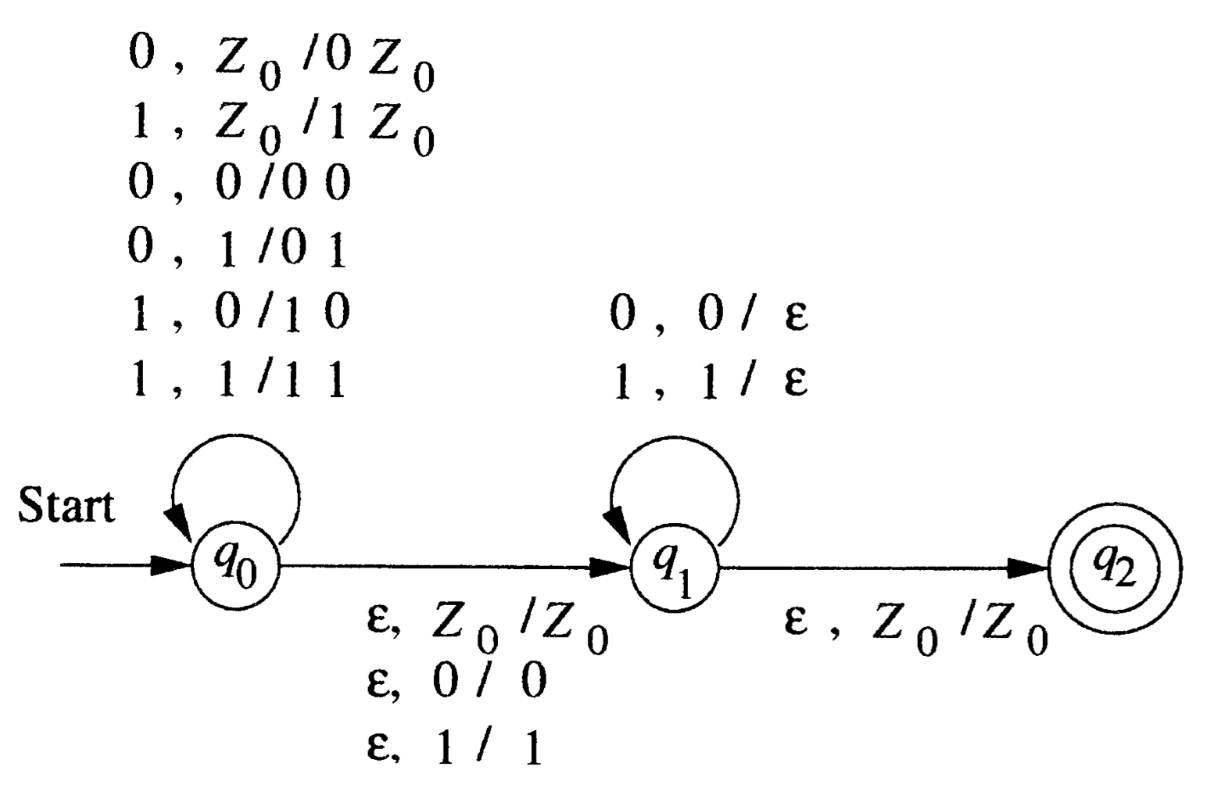
\includegraphics[width=0.5\textwidth]{pda_diag.jpeg}
\end{figure}
\begin{definition}[Instantaneous Descriptions]
  The \textbf{ID} of a PDA is the triple $\left( q,\omega,\gamma \right) $ such
  that $q$ is the current state, $\omega$ the remaining input and $\gamma$ the
  stack contents.
\end{definition}

\begin{notation}[$\vdash$]
  If $\left( p,\alpha \right) \in \delta\left( q,a,X \right)$, we denote
  \[\left( q,a\omega,X,\beta \right) \vdash \left( p,\omega,\alpha\beta
  \right)\qquad \forall \omega\in \Sigma^{*},\beta\in \Gamma^{*}.\]
  This represents one move of the PDA.
\end{notation}
\begin{notation}[$\vdash^{*}_P$]
  To represent zero or moves of the PDA, we further define the relation $\vdash^{*}_P$:
  \begin{enumerate}
    \item \textit{Base Case}: $I\vdash^{*}_P I$ 
    \item \textit{Inductive Step}: For IDs $I,J$, if $\epsilon$ some ID $K$
      such that $I\vdash K$ and $K\vdash^{*}_P J$, then $I\vdash^{*}_P J$
  \end{enumerate}
\end{notation}

\subsubsection{Language of a PDA}
\begin{definition}[Language of a PDA]
  The \textit{language} of a PDA $P$ is denoted $L(P)$ and depends on the modality of acceptance
  of the PDA\@. It is defined by
  \[\left\{ \omega|\left( q_0,\omega,Z_0 \right) \vdash_P^{*}\left( q_f,\epsilon,\alpha \right) \right\},q_f\in F \quad\text{ for acceptance by final state.}.\] 
  \[\left\{ \omega|\left( q_0,\omega,Z_0 \right) \vdash_P^{*}\left( q_f,\epsilon,\epsilon \right) \right\},q_f\in F \quad\text{ for acceptance by empty stack.}.\] 
\end{definition}

\begin{theorem}[Equivalence of Acceptance Modalities]
  The two modalities of acceptance are equivalent, in the sense that $L$ has a
  PDA that accepts it by final state $\iff$ $L$ has a PDA that accepts it by
  empty stack.\\
  Equivalently, the class of languages accepted by final state is equal to the class
  of languages accepted by empty stack.
\end{theorem}
\begin{theorem}
  Suppose a language $L$ has a PDA that accepts it by empty stack. Then $L$ has
  a PDA that accepts it by final state.
\end{theorem}
\begin{proof}
  Suppose $L=L(P_N)$ through acceptance by empty stack for some PDA $P_N=\left(
  Q,\Sigma,\Gamma,\delta_N,q_0,Z_0,F \right) $. Consider the PDA
  \[P_F=\left( Q\cup \left\{ p_0,p_f \right\} ,\Sigma,\Gamma\cup \left\{ X_0
  \right\} ,\delta_F,p_0,X_0,\left\{ p_f \right\}  \right)\]
  such that
  \begin{enumerate}
    \item $P_F$ spontaneously transits to the start state of $P_N$, pushing the start symbol.
      \[\delta_F\left( p_0,\epsilon,X_0 \right) =\left\{ \left( q_0,Z_0 X_0 \right)  \right\}\]
    \item $P_F$ simulates $P_N$.  \[\forall q\in Q,a\in \Sigma\cup \left\{ \epsilon \right\},Y\in
      \Gamma\qquad \delta_N\left( q,a,Y \right) \subseteq \delta_F\left(
    q,a,Y\right) \]
  \item After the stack is empty, transit to the final state of $P_F$.
    \[\forall q\in Q\qquad \left( p_f,\epsilon \right) \in \delta_F\left(
    q,\epsilon,X_0 \right) \]
  \end{enumerate}
  We now show that $w\in L(P_F)\text{ with acceptance by final state } \iff \omega\in L$.\\
  ($\impliedby$) Suppose $\omega\in L$. $\left( q_0,\omega,Z_0 \right) \vdash_{P_N}^{*}$ for
  some state $q$.
  \[\left( q_0,\omega,Z_0X_0 \right) \vdash_{P_N}^{*}\left( q,\epsilon,X_0
  \right).\]
  Since $P_F$ has all the moves of $P_N$, $\left(
  q_0,\omega,Z_0X_0 \right) \vdash_{P_F}^{*}\left(
  q,\epsilon,X_0 \right) $. Hence we have
  \[\left( p_0,\omega,X_0 \right) \vdash_{P_F}\left( q_0,\omega,Z_0X_0 \right) \vdash_{P_F}^{*}\left( q,\epsilon,X_0 \right)\vdash_{P_F}\left( p_f,\epsilon,\epsilon \right)\]
  and $P_F$ accepts $\omega$ by final state.\\
  ($\implies$) Suppose $P_F$ accepts $\omega$ by final state. Since
  transitions to $p_f$ require $X_0$ as the stack symbol, and $X_0$ can only be
  on the bottommost position, any computation of $P_F$ that accepts $\omega$
  must be of the previously shown sequence.  Hence $\omega$ is in $P_N$.
  \begin{figure}[h!]
    \centering
    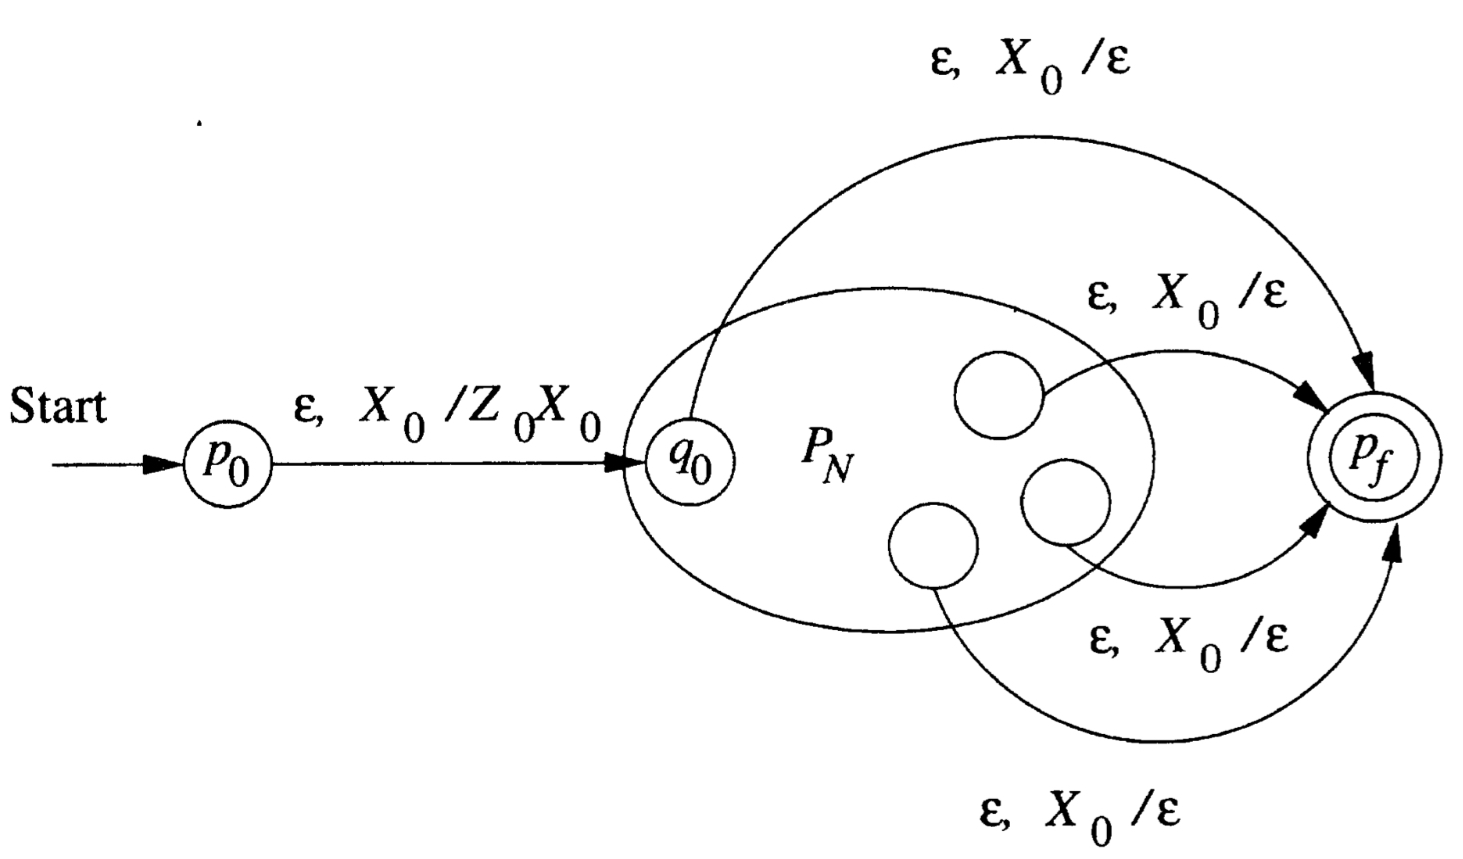
\includegraphics[width=0.6\textwidth]{pda_empty_final.jpeg}
  \end{figure}
  \qed
\end{proof}

\begin{theorem}
  Suppose a language $L$ has a PDA that accepts it by final state. Then $L$ has
  a PDA that accepts it by empty stack.
\end{theorem}
Suppose $L =L(P_F)$ through acceptance by final state for some PDA
$P_F=\left( Q,\Sigma,\Gamma,\delta_F,q_0,Z_0,F \right) $. Consider the PDA
\[P_N=\left( Q\cup \left\{ p_0,p \right\},\Sigma,\Gamma\cup \left\{ X_0 \right\} ,\delta_N,p_0,X_0 \right)\]
such that
\begin{enumerate}
\item We push the start symbol of $P_F$ onto the stack and going to the start state of $P_F$. \[\delta_N\left( p_0,\epsilon,X_0 \right) =\left\{ q_0,Z_0 X_0 \right\} \]
\item $P_N$ simulates $P_F$. \[\forall q\in Q,a\in \Sigma\cup \left\{ \epsilon \right\},Y\in \Gamma\qquad \delta_F\left( q,a,Y \right) \subseteq \delta_N\left( q,a,Y \right) \]
  \item If $P_F$ accepts, $P_N$ starts emptying its stack without consuming
    input. \[\forall q\in F,Y\in \Gamma\cup \left\{ X_0 \right\}\qquad \left(
  p,\epsilon \right) \in \delta_N\left( q,\epsilon,Y \right) \]
  \item After $P_F$ has accepted, $P_N$ pops every symbol until the stack is
    empty. \[\forall Y\in \Gamma\cup \left\{ X_0 \right\}\qquad \delta_N\left(
    p,\epsilon,Y \right) =\left\{ \left( p,\epsilon \right)  \right\} \]
\end{enumerate}
\begin{figure}[h!]
  \centering
  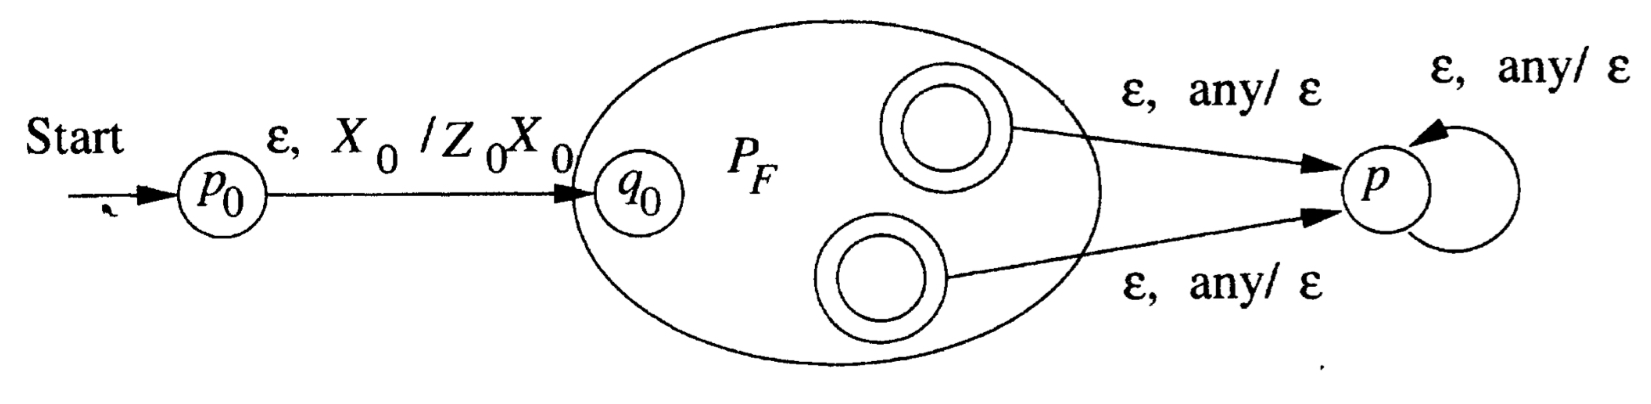
\includegraphics[width=0.6\textwidth]{pda_final_empty.jpeg}
\end{figure}
It can be shown that $\omega\in L(P_N)$ with acceptance by empty stack $\iff\omega\in L$.
\begin{remark}
  For a given PDA $P$, the languages that $P$ accepts by final state and by
  empty stack are different in general.
\end{remark}


\subsection{CFGs vs PDAs}
\subsubsection{Equivalence of CFGs and PDAs}
\begin{theorem}
  A language $L$ is accepted by some PDA if $L$ is accepted by some CFG\@.
\end{theorem}
\begin{proof}
  Suppose a CFG $G=\left( V,T,G,S \right) $. We construct a PDA $P$ as follows: 
  \[P=\left( \left\{ q \right\} ,T,V\cup T,\delta,q,S \right)\]
  where $\delta$ is defined:
  \begin{enumerate}
    \item For each nonterminal $A\in V$, $\delta\left( q,\epsilon,A \right)
      =\left\{ \left( q,\beta \right) | A\to \beta\in G \right\}$
    \item For each terminal $a\in T$, $\delta\left( q,a,a \right) =\left\{ q,\epsilon \right\} $
  \end{enumerate}
  We prove that $\omega\in L(G)\iff \omega\in L(P)$ with
  acceptance by empty stack.\\

  ($\implies$) Suppose $\omega\in L(G)$. Then $\omega$ has a leftmost derivation
  \[S = \gamma_1 \Rightarrow \gamma_2 \Rightarrow \cdots \Rightarrow \gamma_{n}=\omega.\] 
  We show by induction on $i$ that $\left( q,\omega,S \right) \vdash^{*} \left(
  q,y_i,\alpha_i \right) $, where $\gamma_i=x_i\alpha_i$, $\omega=x_i y_i$,
  $x_i,y_i\in T^{*}$ and $\alpha\in \left( V\cup T \right) ^{*}$. That is,
  $\alpha_i$ is the tail of $\gamma_i$ from the first nonterminal (from the
  left), and $y_i$ is the nonterminal string to be generated from $\alpha_i$.
  \begin{enumerate}
    \item \textit{Basis Step:} $\gamma_1=S$, $x_1=\epsilon$, $y_1=\omega$. By definition,
      $\left( q,\omega,S \right) \vdash^{*}\left( q,\omega,S \right) $.
    \item \textit{Inductive Step:} Suppose by inductive hypothesis that $\left(
      q,\omega,S \right) \vdash^{*}\left( q,y_i,\alpha_i \right) $. $\alpha_i$
      begins with a nonterminal $A$. By replacing $A$ by one of its production
      bodies, say $\beta$ with rule (1) of $\delta$, and removing all terminals at the
      top of the stack with rule (2) of $\delta$, we reach the ID $\left(
      q,y_{i+1},\alpha_{i+1} \right) $.
  \end{enumerate}
  Since $\omega$ is a string of terminals, $\alpha_{n}=\epsilon$, and we have
  $\left( q,\omega,S \right) \vdash^{*}\left( q,\epsilon,\epsilon \right) $.
  $P$ accepts $\omega$ by empty stack.\\

  ($\impliedby$) Suppose $\left( q,x,A \right) \vdash^{*}\left(
  q,\epsilon,\epsilon \right) $. Inducting on the number of moves taken by $P$,
  we have:
  \begin{enumerate}
    \item \textit{Basis Step:} $A\to\epsilon$ is a production of $G$, and the
      move is of rule (1). We have $x=\epsilon$ and $A \Rightarrow \epsilon$.
    \item \textit{Inductive Step:} Suppose $P$ takes $n$ moves. The first move
      must be of rule (1), where $A$ is replaced by one of its production
      bodies. Let the production used be $A\to Y_1 Y_2 \cdots Y_k$ for some
      $Y_i\in \left( V\cup T \right)^{*}$. By taking $x=x_1 x_2\cdots x_k$,
      where each $x_i$ is the portion of the input consumed until $Y_1$ is
      popped off the stack, for all $i=1,2,\ldots,k$:
      \[\left( q,x_i x_{i+1}\cdots x_k,Y_i \right) \vdash^{*}\left(
      q,x_{i+1}\cdots x_k,\epsilon \right).\]
      Each of these sequences are no more than $n-1$ moves (since the PDA
      completes in $n-1$ moves), $Y_i \Rightarrow ^{*}x_i$ for nonterminals
      $Y_i$. For terminals $Y_i$, only one move is involved, matching the one
      symbol against $Y_i$. Hence we have the derivation:
      \[A \Rightarrow Y_1 Y_2\cdots Y_k \Rightarrow ^{*}x_1Y_2\cdots Y_k \Rightarrow ^{*}\cdots \Rightarrow^{*} x_1x_2\cdots x_k.\]
      We have $A \Rightarrow ^{*}x$.
  \end{enumerate}
  By letting $A=S$ and $x=\omega$, since $\omega\in L(P)$ by acceptance by empty stack,
  $S \Rightarrow \omega$ and it is in $L(G)$.\qed
\end{proof}
\begin{theorem}
  A language $L$ is accepted by some CFG if $L$ is accepted by some PDA\@.
\end{theorem}
\begin{proof}
  Suppose a PDA $P=\left( Q,\Sigma,\Gamma,\delta,q_0,Z_0 \right)$ accepting by
  empty stack. We construct a CFG as follows:
  \[G=\left( V,\Sigma,R,S \right)\]
  where $V=\left\{ S \right\} \cup \left\{ \left[ pXq \right] |p,q\in Q,Z\in
  \Gamma \right\} $. Each nonterminal encodes the `net popping' of symbol $X$
  from the stack, with a change in state from $p$ to $q$. The productions of
  $G$ are then:
  \begin{enumerate}
    \item $\forall p\in Q$, $S\to\left[ q_0Z_0p \right] \in R$. That is, we
      generate all strings that pop $Z_0$ while going from state $q_0$ to (any)
      state $p$, $\left( q_0,\omega,Z_0 \right) \vdash^{*}\left(
      p,\epsilon,\epsilon \right) $.
    \item If $\left( r,Y_1Y_2\cdots Y_k \right) \in \delta\left( q,a,X \right) $, where $a\in \Sigma\cup \left\{ \epsilon \right\}, k\in \mathbb{N}$, 
      \[\forall \left( r_1,r_2,\ldots,r_k \right) \in Q^{k},\qquad \left[ qXr_k
      \right] \to a\left[ rY_1r_1 \right] \left[ r_1Y_2r_2 \right]\cdots\left[
    r_{k-1}Y_kr_k \right].\] 
    Intuitively, one of the ways to pop $X$ and go from states $q$ to $r_k$ is
    to read $a$ and then use some input to sequentially pop each of the
    produced symbols.
  \end{enumerate}
  We prove that $\left( q,\omega,X \right) \vdash^{*}\left( p,\epsilon,\epsilon
  \right)\iff\left[ qXp \right] \Rightarrow ^{*}\omega$.\\

  ($\implies$) Suppose $\left( q,\omega,X \right) \vdash^{*}\left(
  p,\epsilon,\epsilon \right)$. Inducting on the number of moves taken by $P$, we have:
  \begin{enumerate}
    \item \textit{Basis Step:} With one step, $\left( p,\epsilon \right) \in \delta\left( q,\omega,X \right)$ and $\omega$ is a single symbol or $\epsilon$. By construction, $\left[ qXp \right] \to \omega$ is a production and $\left[ qXp \right] \Rightarrow \omega$.
    \item \textit{Inductive Step:} Suppose the sequence $\left( q,\omega, X
      \right) \vdash^{*}\left( p,\epsilon,\epsilon \right) $ takes $n>1$ steps.
      The sequence must be of the form
      \[\left( q,\omega, X \right) \vdash \left( r_0,x,Y_1Y_2\cdots Y_k \right)
      \vdash^{*}\left( p,\epsilon, \epsilon \right)\] 
      where $\omega=ax$, $a\in \left\{ \epsilon \right\} \cup \Sigma$. We have 
      $\left( r_0,Y_1Y_2\cdots Y_k \right)\in \delta\left( q,a,X \right) $ and
      by construction, we have the productions $\left[ qXp \right] \to a\left[
      r_0Y_1r_1 \right] \left[ r_1Y_2r_2 \right] \cdots\left[ r_{k-1}Y_k p
      \right] $ for all states $r_1,r_2,\ldots,r_k\in Q$. Let
      $x=\omega_1\omega_2\cdots\omega_k$ where each $\omega_i$ is the input consumed to
      `pop' $Y_i$ off the stack. We have the sequences of less than $n$ moves $\left( r_{i-1},\omega_i,Y_i \right)
      \vdash{*}\left( r_i,\epsilon,\epsilon \right)$ and hence $\left[
      r_{i-1}Y_ir_i \right] \Rightarrow
      ^{*}\omega_i$ by inductive hypothesis.
      \[\left[ qXr_k \right] \Rightarrow a\left[ r_0Y_1r_1 \right] \left[
      r_1Y_1r_2 \right] \cdots\left[ r_{k-1}Y_kp \right] \Rightarrow
    ^{*}aw_1\left[ r_1Y_2r_2 \right] \left[ r_2Y_3r_3 \right] \cdots\left[
  r_{k-1}Y_kp \right] \Rightarrow ^{*}aw_1w_2\cdots w_k.\]
  \end{enumerate}
  We have $\left[ qXp \right]\Rightarrow ^{*}\omega$.\\
  
  ($\impliedby$) Suppose $\left[ qXp \right] \Rightarrow ^{*}\omega$. Inducting
  on the number of steps in the derivation, we have:
  \begin{enumerate}
    \item \textit{Basis Step:} With one step, $\left[ qXp \right] \to \omega$
      is a production $\iff$ there is a transition of $P$ in which $X$ is
      popped and we transit states from $q$ to $p$. $\left( p,\epsilon \right)
      \in \delta\left( q,a,X \right) $ and $a=\omega$, hence $\left( q,\omega,X
      \right) \vdash \left( p,\epsilon,\epsilon \right) $.
    \item \textit{Inductive Step:} Suppose $\left[ qXp \right] \Rightarrow
      ^{*}\omega$ by $n>1$ steps. The derivation must be of the form
      \[\left[ qXp \right] \Rightarrow a\left[ r_0Y_1r_1 \right] \left[
      r_1Y_2r_2 \right] \cdots\left[ r_{k-1}Y_kp \right]\Rightarrow
    ^{*}\omega.\]
    We have $\left( r_0,Y_1Y_2\cdots Y_k \right) \in \delta\left( q,a,X \right) $.
    Let $\omega=a\omega_1\omega_2\cdots\omega_k$ such that $\left[
    r_{i-1}Y_ir_i \right] \Rightarrow ^{*}\omega_i$. By inductive hypothesis,
    $\left( r_{i-1},w_i,Y_i \right) \vdash^{*}\left( r_i,\epsilon,\epsilon
    \right) $ for each $i$. This gives us
    \[\left( q,a\omega_1\omega_2\cdots\omega_k,X \right) \vdash\left(
    r_0,\omega_1\omega_2\cdots\omega_k,Y_1Y_2\cdots Y_k \right)\vdash
  ^{*}\left( r_1,\omega_2\omega_3\cdots\omega_k,Y_2Y_3\cdots Y_k \right)\vdash
^{*}\cdots\vdash ^{*}\left( p,\epsilon,\epsilon \right).\] 
  \end{enumerate}
  Since $S\Rightarrow ^{*}\omega\iff\left[ q_0Z_0p \right]
  \Rightarrow ^{*}\omega$ for some state $p$ (by construction), and each
  $\left[ q_0Z_0p \right]\Rightarrow ^{*}\omega\iff\left( q_0,\omega,Z_0
  \right) \vdash^{*}\left( p,\epsilon,\epsilon \right) $, we have $L(G)=L(P)$
  with acceptance by empty stack.
\end{proof}

\subsection{Context Free Languages}
To show that a given language is non context-free, we may use the pumping
lemma. Intuitively, in any sufficiently long string, it is possible to find two
short nearby substrings that we can ``pump'' in tandem, while keeping the
resulting string in $L$.
\begin{lemma}
  Let $L$ be a CFL\@. Then $\exists n=f(L)$ such that $\forall z\in L$,
  $\left| z \right| \ge n$, $\exists u,v,w,x,y\in \Sigma^{*},z=uvwxy$ such that:
  \begin{enumerate}
    \item $\left| vwx \right| \le n$. That is, the two strings to be ``pumped''
      is not too far from the other.
    \item $vx\neq\epsilon$. At least one of the strings to be ``pumped'' cannot be empty.
    \item $\forall i\ge 0$, $uv^{i}wx^{i}y\in L$
  \end{enumerate}
\end{lemma}
The contrapositive of the lemma is used to prove that a language is
not context-free. That is, $\forall n\in \mathbb{N}$, $\exists z\in L$, such
that $\left| z \right| \ge n$, $\forall u,v,w,x,y\in \Sigma^{*}$, where
$z=uvwxy$, $\left| vwx \right| \le n$, $vx\neq\epsilon$, we have
\[\exists i\in \mathbb{N}\left( uv^{i}wx^{i}y\notin L \right)\]

\begin{proof}
  Suppose $L$ is context-free. Without loss of generality, assume
  $L\neq\emptyset $, $L\neq\left\{ \epsilon \right\} $ and a CNF grammar
  $G=\left( V,T,P,S \right) $ for $L-\left\{ \epsilon \right\} $. Let $m=\left|
  V \right| $ and $n=2^{m}$. Consider a string $z\in L$ such that $\left| z
  \right| \ge n$.  Its parse tree must have a path from the
  root to a leaf of length at least $m+1$. By Pigeonhole Principle, there must
  exist a repeated nonterminal $A$.\\

  We have the derivation of the form, where $z=uvwxy$ for some $u,v,w,x,y\in \Sigma^{*}$,
  \[S\Rightarrow ^{*}uAy\Rightarrow ^{*}uvAxy\Rightarrow ^{*}uvwxy.\]
  \begin{figure}[h!]
    \centering
    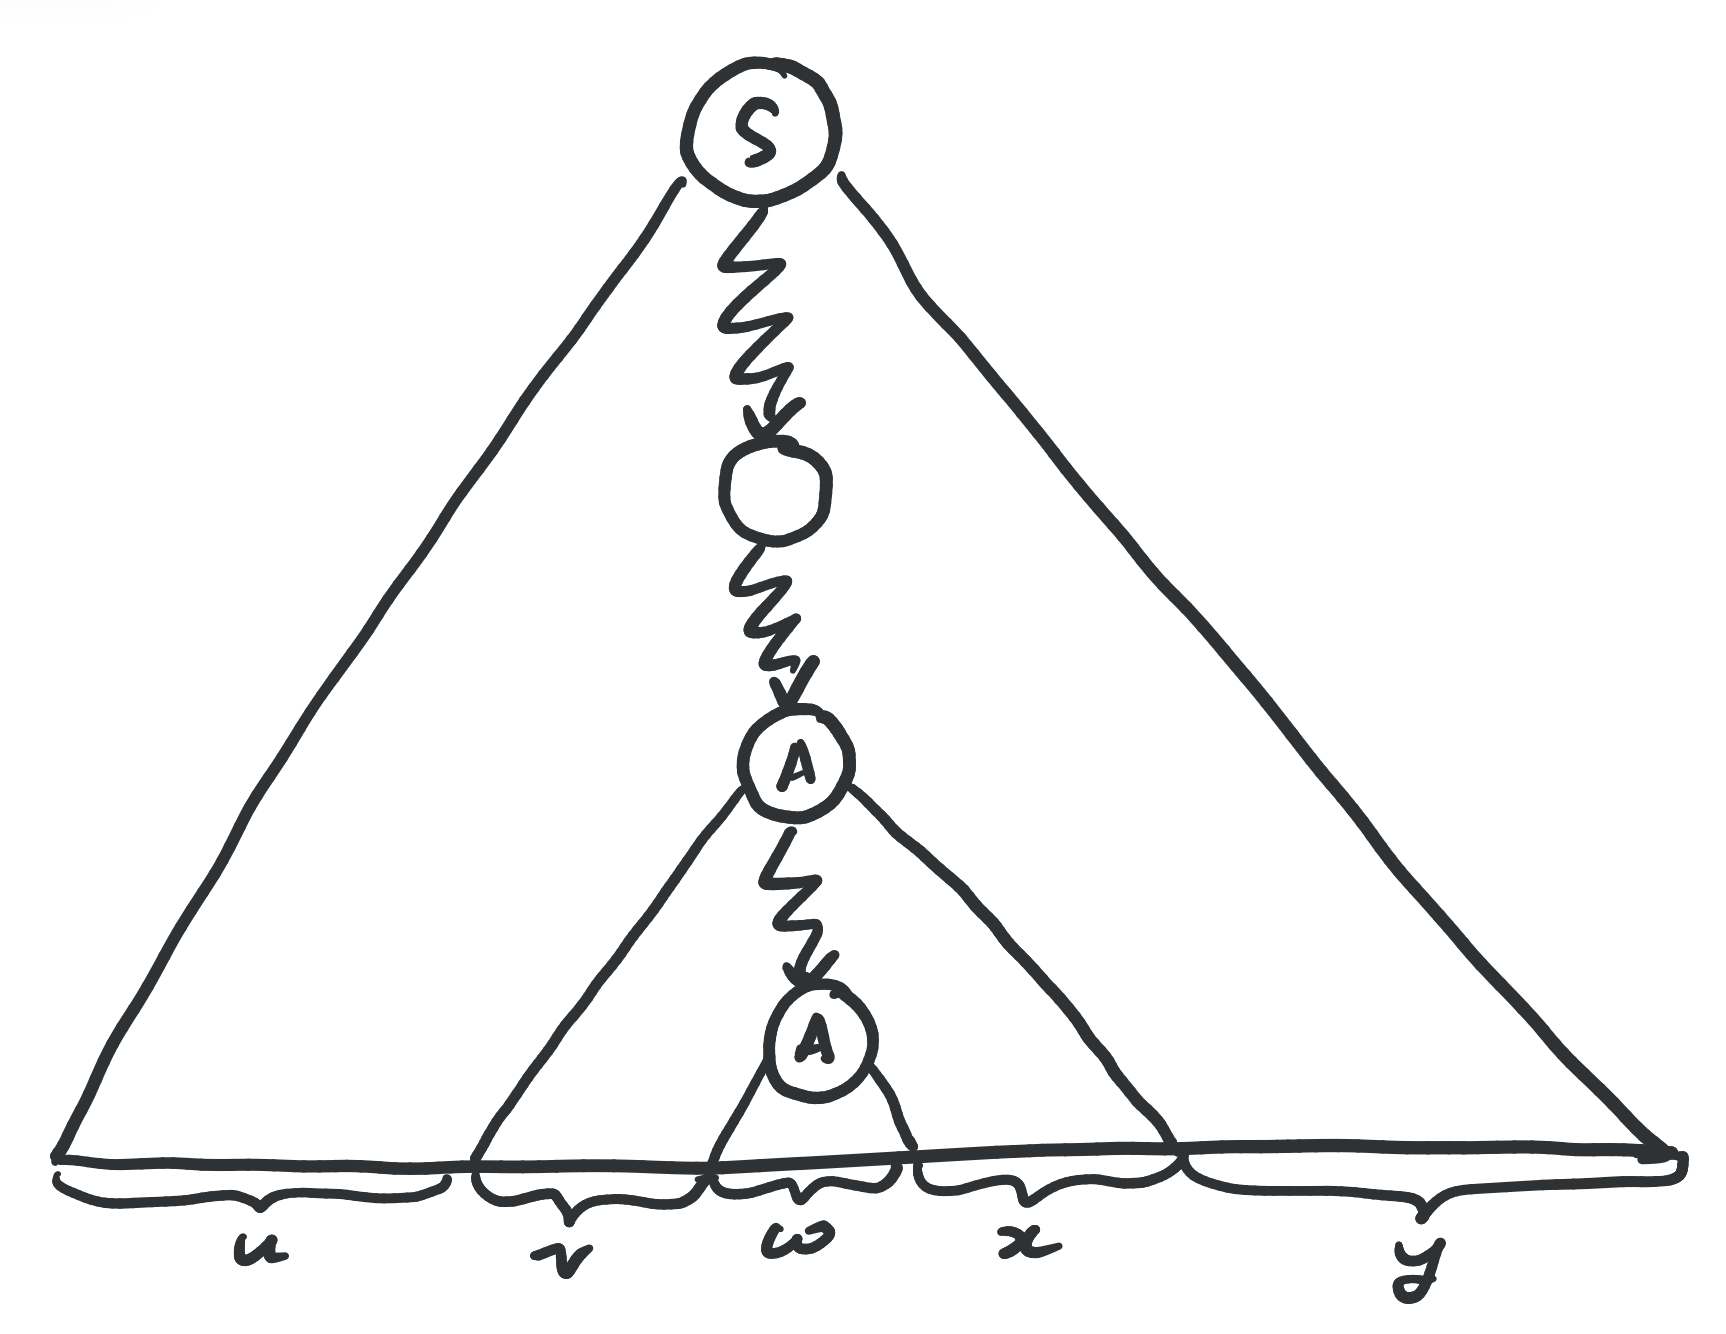
\includegraphics[width=0.5\textwidth]{cfl_pumping_lemma}
  \end{figure}

  Additionally, we have $A\Rightarrow ^{*}vAx$ and $A\Rightarrow ^{*}w$. For
  any $i\in \mathbb{N}$, we thus may have the derivation
  \[S\Rightarrow ^{*}uAy\Rightarrow ^{*}uv^{i}Ax^{i}y\Rightarrow ^{*}uv^{i}wx^{i}y.\]
  With the assumption that the grammar is of CNF, since the repeated terminals
  are maximally $m$ production steps apart, we have the length $\left|  vwx
  \right| \le n$, and since the derivation $A\Rightarrow ^{*}vAx$ uses at least
  one production step, $vx\neq \epsilon$.\\

  For the excluded cases when constructing the CNF grammar, the statement of
  the pumping lemma is vacuously true for $L=\emptyset $ and we choose $n$ such
  that $z\neq\epsilon$ for $L=\left\{ \epsilon \right\} $.
  \qed%
\end{proof}

By using the pumping lemma, we can construct a proof of the following structure to show a specified language is non context-free:

\begin{prop}
  $L=\left\{ a^{m}b^{m}c^{m} | m\ge 1\right\} $ is not context-free.
\end{prop}
\begin{proof}
  Suppose $L$ is regular. Let $n$ be as in the Pumping Lemma. Let
  $z=a^{n}b^{n}c^{n}$. Let $z=uvwxy$ as in the pumping lemma. Since $\left| vwx
  \right| \le n$, $vwx$ cannot contain both $a$ and $c$. \\

  Suppose $vwx$ does not contain $a$'s. By the pumping lemma, $uv^{2}wx^{2}y\in
  L$. But $uv^{2}wx^{2}y$ contains $n$ $a$'s, and $\left| uv^{2}wx^{2}y \right|
  >3n$, hence $uv^{2}wx^{2}y\not\in L$.\\

  Suppose $vwx$ does not contain $c$'s. Similarly, By the pumping lemma,
  $uv^{2}wx^{2}y\in L$. But $uv^{2}wx^{2}y$ contains $n$ $c$'s, and $\left|
  uv^{2}wx^{2}y \right| >3n$, hence $uv^{2}wx^{2}y\not\in L$.\\

  Hence $L$ is non context-free.\qed%
\end{proof}

\begin{prop}
  $L=\left\{ \alpha\alpha|\alpha\in \left\{ a,b \right\} ^{*} \right\} $ is not
  context-free.
\end{prop}

\begin{lemma}[Ogden's Lemma]
  Let $L$ be a CFL. Then $\exists n$ such that $\forall z\in L$, $\left| z
  \right| \ge n$, $\exists u,v,w,x,y\in \Sigma^{*}$, $z=uvwxy$, if $\ge n$ positions
  in $z$ are marked as distinguished,
  \begin{itemize}
    \item $vwx$ has at most $n$ distinguished positions.
    \item $vx$ has at least $1$ distinguished position.
    \item $\forall i\ge 0$, $uv^{i}wx^{i}y\in L$.
  \end{itemize}
\end{lemma}
Ogden's Lemma provides an stronger form of the pumping lemma that can be used
to prove non-context free-ness.

\subsubsection{Closure of Context-Free Languages}
We have, similarly to regular languages, certain operations that, when applied to CFLs,
the resulting language is also a CFL\@.

\begin{definition}[Substitution]
  Suppose terminals $i$ and CFLs $L_i$. Consider a mapping
  $s:\Sigma\to\mathcal{P}\left( \Gamma^{*} \right) $ such that $s(i)=L_i$, that
  is further defined for strings by principle of induction:
  \begin{enumerate}
    \item \textit{Base Case:} $s(\epsilon)=\left\{ \epsilon \right\}$
    \item \textit{Inductive Case:} $s(\omega a)=s(\omega)\cdot s(a), \forall a\in \Sigma,\omega\in \Sigma^{*}$
  \end{enumerate}
  $s$ is called a \textit{substitution}. Intuitively, we replace each symbol in the
  strings of one language by an entire language.
\end{definition}
\begin{theorem}
  Given a CFL $L$ over $\Sigma$ and $s$ a substitution on $\Sigma$ such that
  $s\left( a \right) $ is a CFL for each $a\in \Sigma$, $s\left( L \right) $ is
  a CFL.
\end{theorem}
The principle of the proof is to consider replacing each terminal in the
original grammar with a nonterminal that acts as the start symbol of the
substituted CFL. We then have a resultant CFG that generates $s\left( L \right)
$.\\

Given CFLs $L,L_1,L_2$ and regular language $R$:
 \begin{itemize}
  \item $L_1\cup L_2$ is context-free.
  \item $L_1\cdot L_2$ is context-free.
  \item $L^{*}$ is context-free.
  \item $L^{+}$ is context-free.
  \item $h\left( L \right) $ is context-free, for some homomorphism $h$.
  \item $L^{R}$ is context-free. Consider the reverse of all productions.
  \item $L\cap R$ is context-free. Consider the PDA for $L$, and DFA for
    $R$. We can simulate the DFA with the analogue for parallelisation of
    DFAs.
  \item $h^{-1}\left( L \right) $ is context-free, for some homomorphism $h$.
\end{itemize}

\begin{remark}
  $\bar{L}$ and $L_1-L_2$ are not necessarily context-free.
\end{remark}

\begin{remark}
  CFLs are not closed under intersection. Consider the CFLs $L_1=\left\{
  0^{n}1^{n}2^{i}|n\ge 1,i\ge 1 \right\} $ and $L_2=\left\{
0^{i}1^{n}2^{n}|n\ge 1,i\ge 1 \right\} $. We have the intersection $L=\left\{
0^{n}1^{n}2^{n}|n\ge 1 \right\} $ which is not context-free.
\end{remark}

\subsubsection{Decision Problems of CFLs}
We may examine some decision problems of CFLs. However, in CFLs, we have to
take into account the complexities of converting between the various forms of
representation, that is required for their decision problems.\\

We have the linear time conversions from a CFG to a PDA, from a PDA accepting
by final state to a PDA accepting by empty stack and vice-versa. On the other hand, the
conversion from a PDA to a CFG is requires an upper bound of $O(n^{3})$ on the
constructed grammar's length and hence running time. Additionally, to convert a
general CFG to its CNF requires $O(n^{2})$ for the length of the resultant
grammar, and running time to construct the unit pairs and eliminate unit
productions.\\

Given these conversions, we are still highly limited in what we may decide
about a CFL, many of which is undecideable as shown in a later chapter.\\

We may check the \textbf{emptiness of CFLs} by running the algorithm to find
all generating symbols in its CFG and checking whether the start symbol $S$ is
generating. That is,
\begin{gather*}
  L=\emptyset \iff  S\text{ is not generating}
\end{gather*}

We may decide the \textbf{membership of a string} $\omega=a_1a_2\cdots a_{n}$
in a CFL $L$. This can be done with dynamic programming, using the CYK
algorithm using a CNF grammar for the language. We construct a triangular table
where each entry $X_{ij}$ is the set of variables $A$ such that $A\Rightarrow
^{*}a_ia_{i+1}\cdots a_j$.
\begin{figure}[h!]
  \centering
  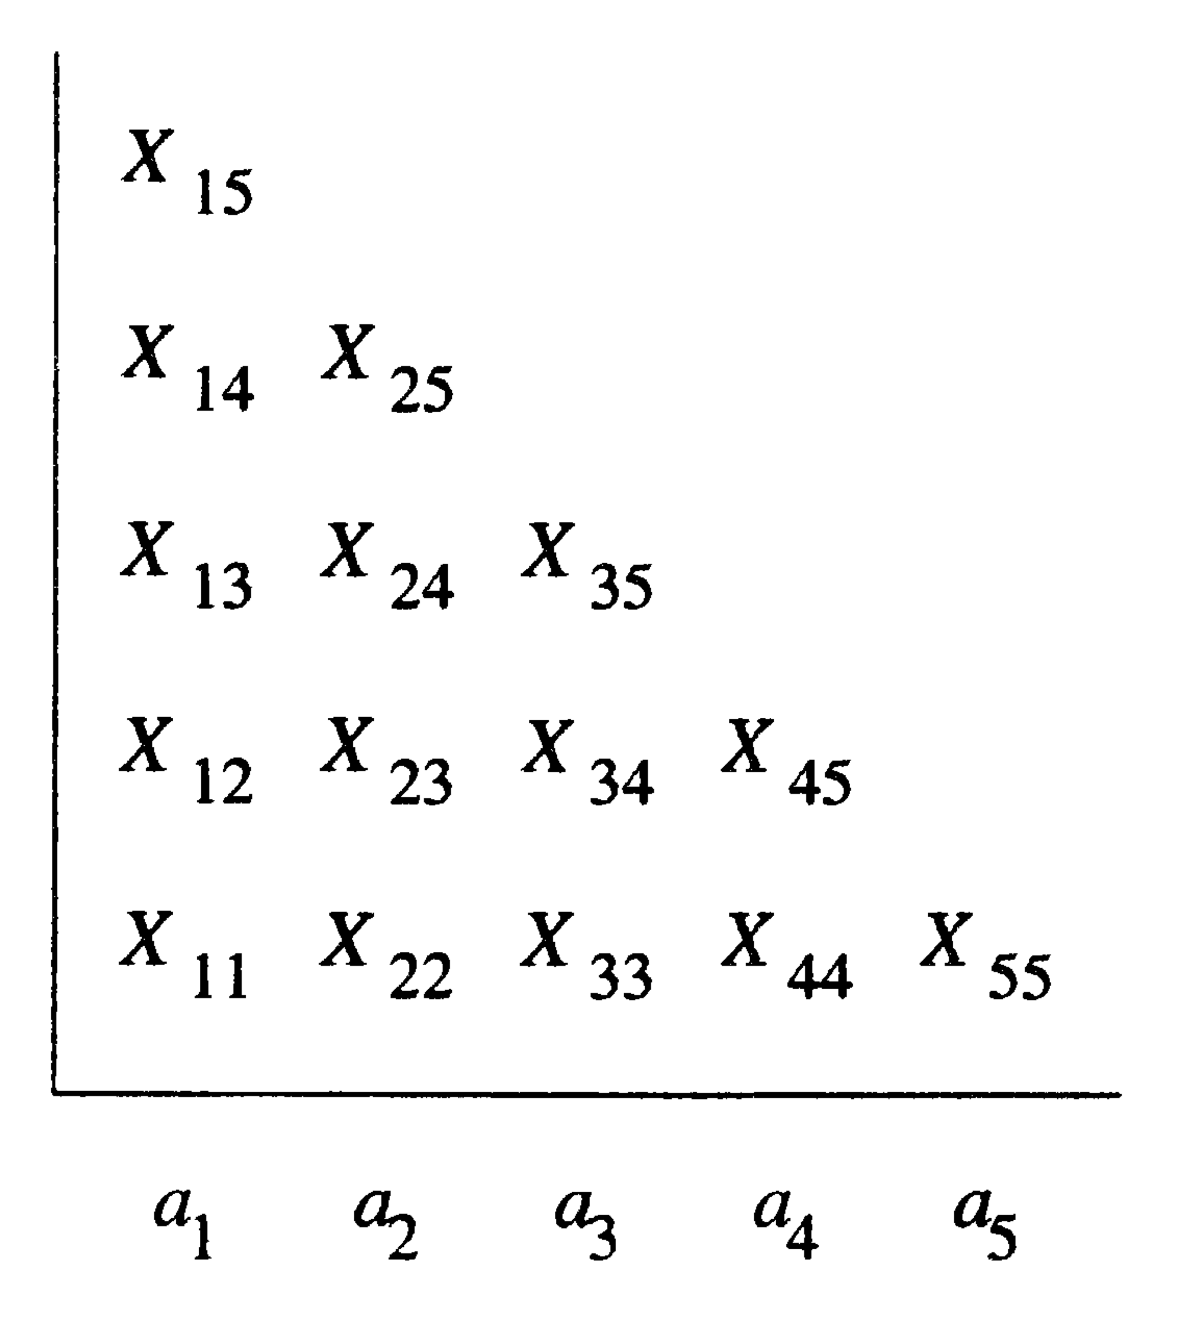
\includegraphics[width=0.3\textwidth]{cyk_algo}
  \captionsetup{labelformat=empty}
  \caption{Table constructed by CYK Algorithm for $n=5$}
\end{figure}\\
We compute the rows bottom-up, with the following inductive algorithm:
\begin{enumerate}
  \item \textit{Base Case:} Each $X_{ii}$ is the set of nonterminals which generate $a_i$
  \item  \textit{Inductive Step:} $X_{i,j}$ contains all $A$ such that $A\to BC
    $, where $B\in X_{i,k}$ and $C\in X_{k+1,j}$ for some $i\le k<j$.
\end{enumerate}
We then have the membership of the string if the start symbol generates the
full length of the string. That is,
\[\omega\in L\iff S\in X_{1,n}\]
\begin{remark}
  The running time of the CYK algorithm is $O(n^{3})$, in comparison to naive
  recursive searches for membership of strings which require exponential time.
\end{remark}

\begin{remark}
  The following CFL decision problems are undecideable:
  \begin{itemize}
    \item Is a given CFG $G$ ambiguous?
    \item Is a given CFL inherently ambiguous?
    \item Is the intersection of two CFLs empty?
    \item Are two CFLs the same?
    \item Is a given CFL equal to $\Sigma^{*}$?
    \item Is a given CFL a regular language?
  \end{itemize}
\end{remark}

\subsection{Deterministic PDA}
PDAs are nondeterministic by definition. However, parsers generally behave
deterministically, and not unlike a deterministic PDA\@. We investigate, in this
section, the behaviour and types of languages accepted by deterministic PDAs.

\begin{definition}[DPDA]
  An PDA $P=\left( Q,\Sigma,\Gamma,\delta,q_0,Z_0,F \right) $ is a \textit{DPDA} if:
  \begin{enumerate}
    \item $\forall q\in Q$, $a\in \left\{ \epsilon \right\} \cup \Sigma$, and
      $X\in \Gamma$,$\qquad\left| \delta\left( q,a,X \right) \right| \le 1$.
      There is only one possible move, if any, for any input and ID.
    \item If $\delta\left( q,\epsilon,X \right)\neq \emptyset\implies\forall
      a\in \Sigma, \delta\left( q,a,X \right)=\emptyset $. That is, we do not
      have a choice between taking a input symbol or making a move on
      $\epsilon$.
  \end{enumerate}
\end{definition}

\subsubsection{Languages Accepted by DPDAs}
We define the languages accepted by DPDAs similarly to that of PDAs.

\begin{theorem}[Languages Accepted by Final State]
  The languages accepted by DPDAs by final state properly include the regular
  languages, but are properly included in the CFLs.
\end{theorem}
On the other hand, DPDAs that accept by empty stack are highly limited, unable
to accept even certain finite languages such as $\left\{ a,aa \right\}$.
\begin{definition}[Prefix Property]
  A language $L$ has the \textit{prefix property} if $\forall \left( x,y
  \right) \in L^{2}$, $x\text{ is not a prefix of }y$.
\end{definition}
\begin{theorem}[Languages Accepted by Empty Stack]
  A language $L$ is $L(P)$ by empty stack for some DPDA $P\iff$ $L$ has the
  prefix property $L$ is $L(P')$ by final state for some DPDA $P$.
\end{theorem}

\subsubsection{Unambiguous Grammars}
\begin{theorem}
  If $L=L(P)$ by acceptance through empty stack for some DPDA $P$, $L$ has an
  unambiguous context-free grammar.
\end{theorem}
The typical conversion of CFG from PDA (with nonterminals encoding state
transition and symbol popped) yields an unambiguous context-free grammar.
Intuitively, this is because there is a unique sequence of moves in the DPDA,
and hence there is only one choice of production every step of the leftmost
derivation of each string. There is also only one final state that can be
reached due to the determinism, and hence only one of the initial branches of
$S$ will be consistent with the PDA\@.

\begin{theorem}
  If $L=L(P)$ by acceptance through final state for some DPDA  $P$, $L$ has an
  umabiguous context-free grammar.
\end{theorem}
This can be shown by adding an end marker $\$\not\in\Sigma$ to every string in
$L$, then creating the context free grammar as though for acceptance through
empty stack, and then introducing a production $\$\to\epsilon$.

\section{Turing Machines}
\begin{definition}[Turing Machine]
  A TM $M=\left( Q,\Sigma,\Gamma,\delta,q_0,B,F \right) $, where:
  \begin{itemize}
    \item $Q$: A finite set of states
    \item $\Sigma$: A finite set of input symbols. $\Sigma\subseteq \Gamma$
    \item $\Gamma$: A finite set of tape symbols
    \item $\delta$: A transition function taking as argument a state and stack
      symbol and returns a state, stack symbol to write and direction to move.
      $\delta:Q\times \Gamma\to Q\times \Gamma\times \left\{ L,R \right\} $ 
    \item $q_0$: A start state, $q_0\in Q$ 
    \item $B$: A blank symbol. $B\in \Gamma-\Sigma$
    \item $F$: A set of final states. $F\in \mathcal{P}\left( Q \right) $
  \end{itemize}
  \begin{figure}[h!]
    \centering
    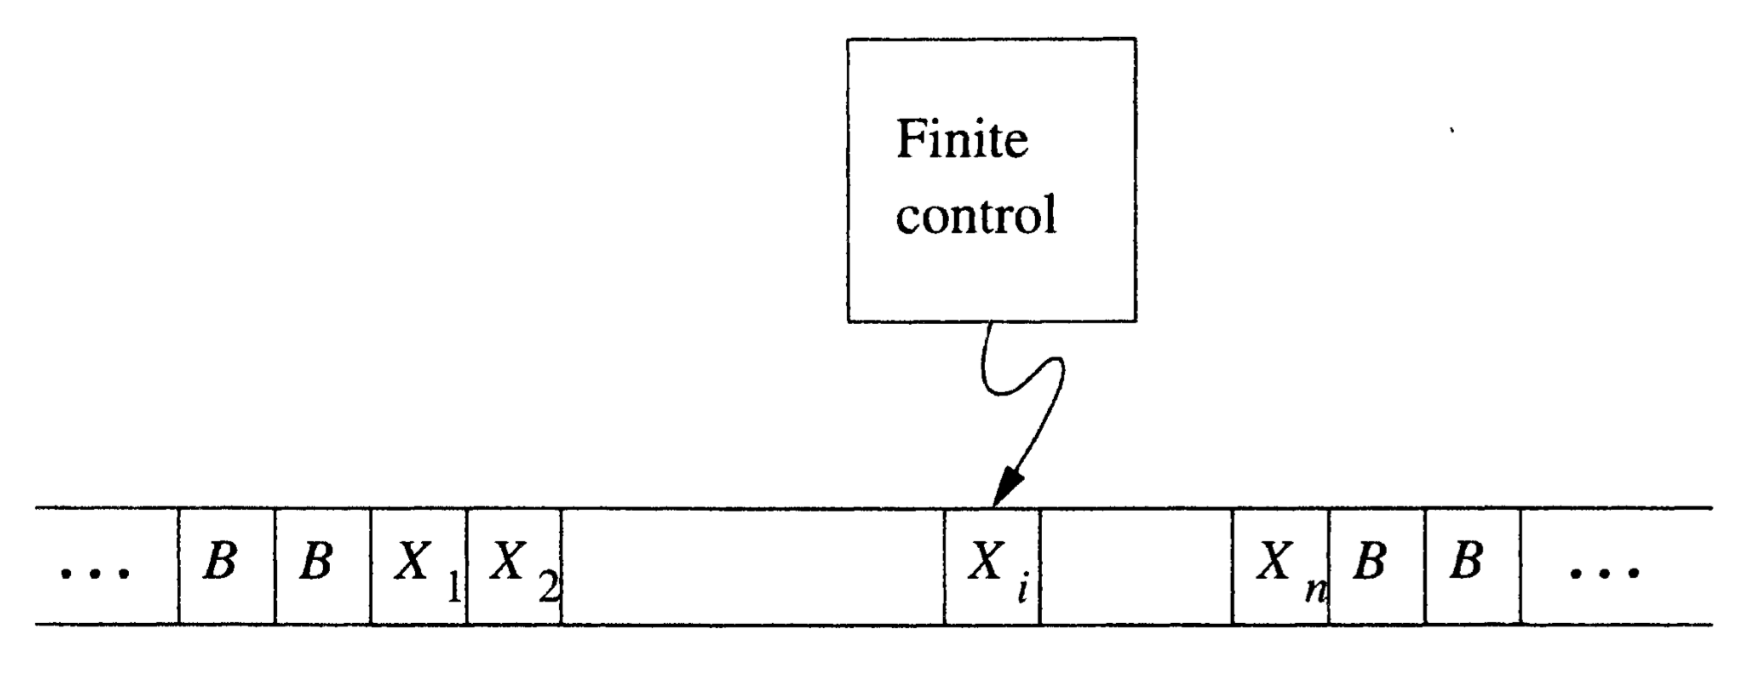
\includegraphics[width=0.5\textwidth]{tm}
  \end{figure}
  A TM consists of a finite control, which can be in any of a finite set of
  states, a infinite tape divided into cells, each holding one of a finite set
  of symbols.\\

  Initially, the input is written on the tape with blank symbols infinitely to
  the left and right of the input. The tape head is positioned on the leftmost
  cell holding an input symbol.\\

  The transition function $\delta$ encapsulates a move of the turing machine,
  consisting:
  \begin{enumerate}
    \item A change in state in the control.
    \item A replacement of the tape symbol in the read cell.
    \item A move to the left or right of the current cell.
  \end{enumerate}
\end{definition}

We have alternative notations for the descriptions of TMs, similarly to DFAs
and PDAs, the transition diagram and table.

\begin{figure}[h!]
  \centering
  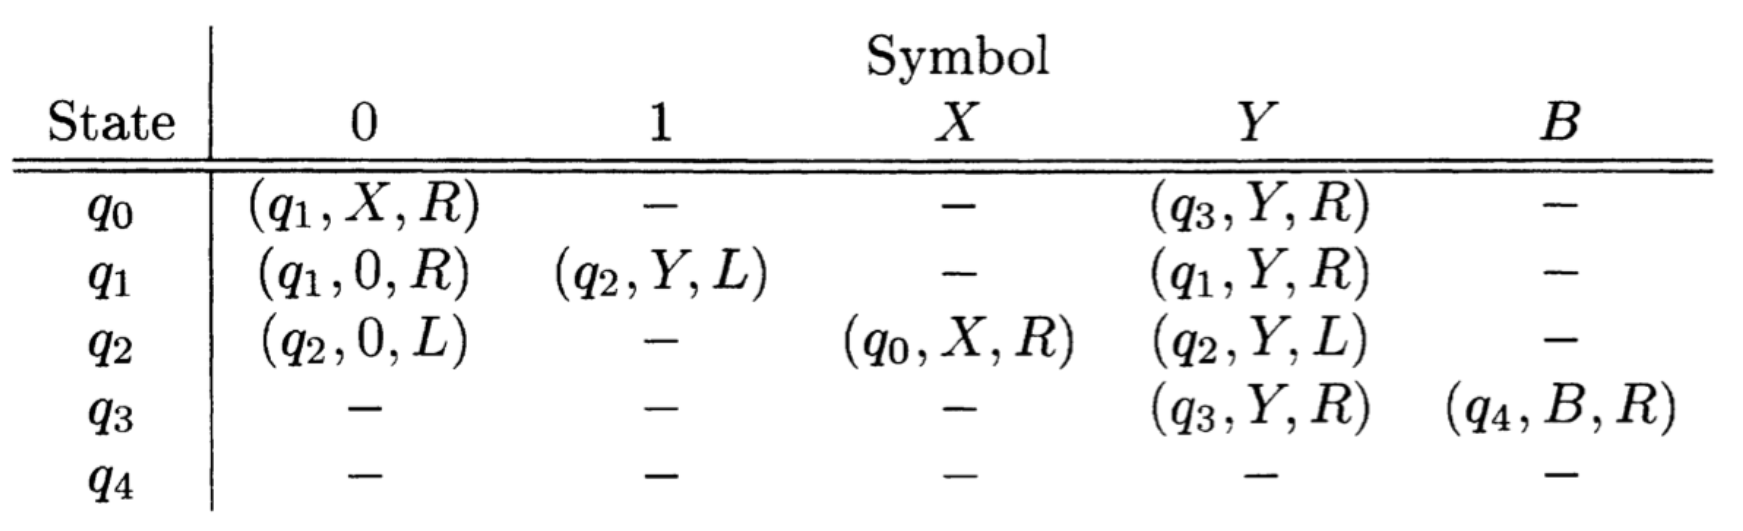
\includegraphics[width=0.6\textwidth]{tm_table}
\end{figure}

We use the transition table to show the moves of the TM, depending on the
current state and tape symbols.

\begin{figure}[h!]
  \centering
  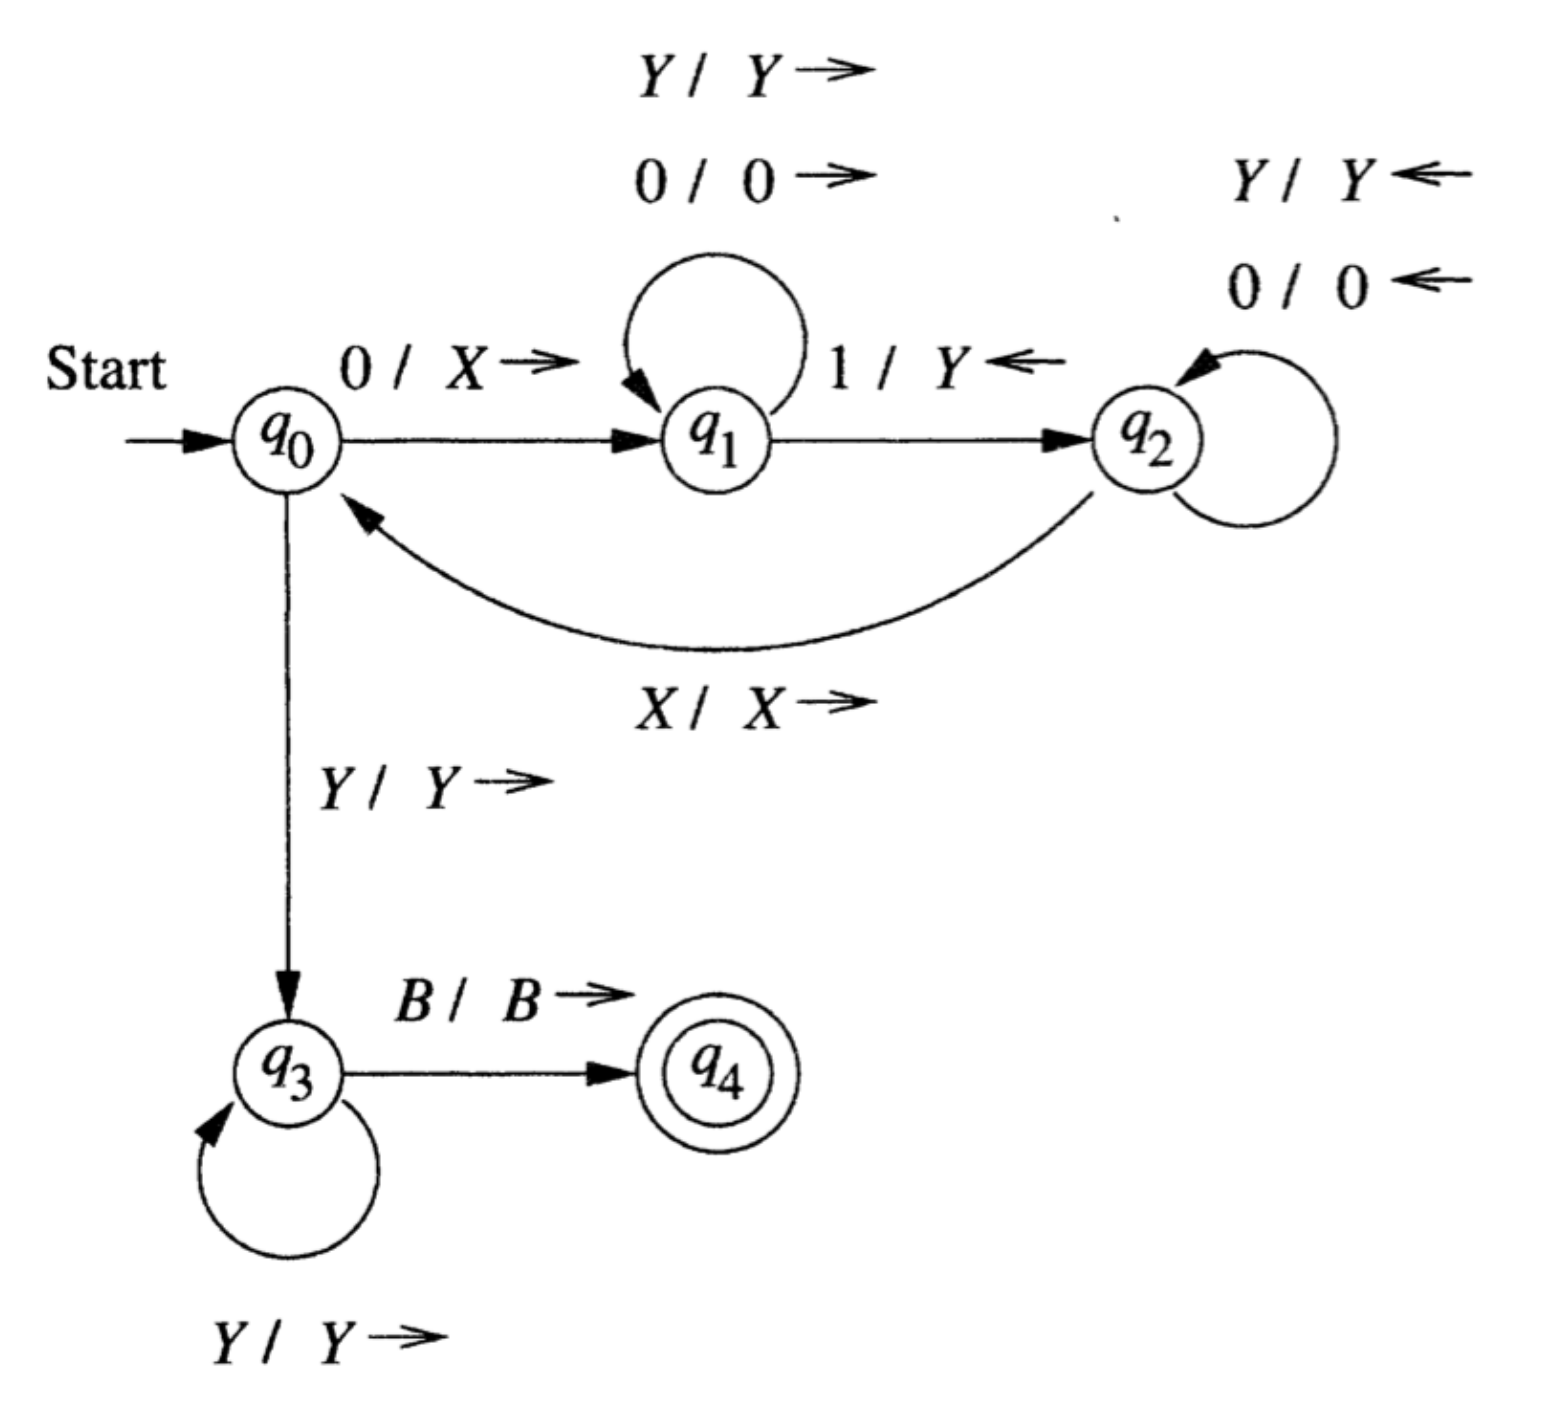
\includegraphics[width=0.5\textwidth]{tm_diag}
\end{figure}

The transition diagram of a TM consists of a set of nodes corresponding to the
states of the TM, within which each arc from state $q$ to $p$ is labelled by
some $X/YD$, where $X,Y\in \Gamma$ and $D\in \left\{ L,R \right\} $.
Additionally, we denote accepting states by double circles and the start state
with an arrow labelled `start' entering that state.

\begin{definition}[Instantaneous Descriptions]
  The \textbf{ID} of a TM, analogous to that of the PDA, is the string
  \[X_1X_2\cdots X_{i-1}q{X}_{i}X_{i+1}\cdots X_{n}.\] 
  where $q$ is the state of the TM, the tape head is scanning the symbol $X_i$
  and $X_1 X_2 \cdots X_{n}$ is the portion of the tape from the leftmost to
  the rightmost nonblank symbols, except if the head is past the ends, in which
  case we extend to show the blank symbols.
\end{definition}

\begin{notation}[$\vdash$]
  If $\delta\left( q,X_i \right) =\left( p,Y,L \right) $, we denote
  \[X_1X_2\cdots X_{i-1} q X_i X_{i+1}\cdots X_{n}\vdash X_1X_2\cdots X_{i-2} q X_{i-1} Y X_{i+1}\cdots X_{n}.\] 
  This represents one move of the TM.
\end{notation}

\begin{notation}[$\vdash^{*}$]
  As usual, we denote $\vdash^{*}$ to represent zero or more moves of the TM.
\end{notation}

\subsection{Turing Machines}
\subsubsection{Acceptance by a TM}
\begin{definition}[Language of a TM]
  The \textit{language} of a TM $M$ is denoted $L(M)$ and is defined by
  \[L(M)=\left\{ x|\exists q_f\in F, q_0x\vdash^{*}\alpha q_f \beta \right\}.\]
  That is, it is the set of strings that, given as input, would eventually
  transit $M$ into an accepting state.
\end{definition}

\begin{definition}[Halting]
  We say a TM halts if it enters a state $q$, scanning a tape symbol $X$, and there
  is no move defined. $\delta\left( q,X \right)$ is undefined.
\end{definition}

\begin{remark}
  By un-defining $\delta\left( q_f, X \right)$ for all final states $q_f$ and
  tape symbols $X$, without changing the language accepted, the TM halts if it
  accepts. We can hence assume that a TM always halts when it accepts a string.
\end{remark}

Since language acceptance is equivalent to function computation, we further
define the notion of function computation on a TM. Provided an input $x$, we
interpret the content of the tape of the TM if/after it halts as the output
$f(x)$.

\subsubsection{Models Equivalent to TMs}
We present certain modifications or improvements to TMs to aid in their
specifications. These modifications do not extend the class of languages
accepted, or extend the basic model of the TM, but only affect running times
and space complexities.

\paragraph{Storage in Finite Control} The finite control not only to represent
a position in the ``program'' of the Turing machine, but also to hold a finite
amount of data. The finite control becomes a tuple of the current state, and
the stored values and variables.

\paragraph{Subroutines} TMs can be thought of as a colection of
``subroutines'', sets of states that perform some useful process. Each
subroutine includes a start state, and a ``return'' state. As such, we may
define general subroutines that that allow us to ``jump'' to a specific return
state depending on the current start state.

\paragraph{Multiple Tapes} The tape of a TM composed of multiple ``tracks''.
Each symbol becomes a tuple of symbols and the tape alphabet consists of tuples
of the original tape alphabet. This TM is hence capable of simulating multiple
tapes.

\paragraph{Nondeterministic TMs} The transition function may instead return a
set of triples, from which the NTM can choose any of the the triples to be the
next move. The language accepted is hence defined as the strings such that,
given as input, there exist a sequence of moves that lead to an ID with an
accepting state.

\begin{theorem}
  If $M_N$ is a nondeterministic TM, there exists a deterministic TM  $M_D$
  such that $L(M_N)=L(M_D)$.
\end{theorem}

Intuitively, in $M_D$, we explore the IDs of $M_N$ ``breadth-first''. That is,
we find all IDs reachable in $0$ moves, then all IDs reachable in $1$ move,
then all IDs reachable in $2$ moves, as so on. This is done with a tape
operating as a queue of IDs to simulate a single move of.\\

We may further consider several restrictions of TMs, that do not affect the
capabilities of TMs.

\paragraph{Semi-Infinite Tapes}  A TM that is infinite only in one
direction (WLOG, to the right) can simulate a TM that is infinite in both
directions. Analogue to the simulation of multiple tapes, we allow each symbol
to be a duple of tape symbols, with each $i$-th cell from the origin be
$(x_{-i}, x_i)$, where $x_i$ is the $i$-th cell from the origin in the original
TM model.

\paragraph{No Blank Symbols Write} The TM is not allowed to write a blank
symbol. This, coupled with semi-infinite tapes, ensure that the tape is at all
times a prefix of nonblank symbols followed by an infinity of blanks. We may
achieve this by creating a new tape symbol $B'$ that effectively functions as
the blank symbol.

\paragraph{Two Stack PDAs} A PDA equipped with two stacks is as powerful as a
TM. We take one stack to simulate the tape symbols to the left of the head, and
the other to simulate the tape symbols to its right. Each move transits the
PDA's state, pops and reads from one stack, and pushes the corresponding output
to the other.


\subsection{Languages of a TM}
Following specifications of TMs and the languages that they accept, we have the
following for the language classes defined by TMs' capabilities. 
\subsubsection{Recursive Enumerable Language}
We first consider the languages that can be accepted by TMs.

\begin{definition}[Recursively Enumerable Languages]
  If $L$ is $L(M)$ for some TM $M$, then $L$ is a \textit{recursively enumerable
  (computably enumerable) language}.
\end{definition}

\paragraph{Codings}
We may define, for a string $x$ over $\left\{ 0,1 \right\} ^{*}$, its coding to be
\[i=\left( 1x \right) _2-1.\]
\begin{notation}
  $\omega_i$ denotes the string with code $i$.
\end{notation}

Further we may define a coding for a TM $M=\left( Q,\Sigma,\Gamma,\delta,q_1,B,\left\{ q_2 \right\}  \right)$ where
\begin{itemize}
  \item $Q=\left\{ q_1,q_2,\ldots,q_{n} \right\} $. If there are multiple
    accepting states, we may define new tape symbols and modify the transition function
    to compress into a single accepting state.
  \item $\Sigma=\left\{ 0,1 \right\} $, WLOG.
  \item $\Gamma=\left\{ X_1,X_2,\ldots,X_s \right\} $, where $X_1=0,X_2=1, X_3=B$.
  \item The directions $L=D_1$ and $R=D_2$.
\end{itemize}
We have, in this way, a coding for any transition
\[\delta\left( q_i,X_j \right) =\left( q_k,X_l,D_m \right)\qquad\to\qquad
0^{i}10^{j}10^{k}10^{l}10^{m}\quad i,j,k,l,m\in \mathbb{N}^*.\]
This allows for a coding for $M$ to be $C_1 11 C_2 11 C_3\ldots C_{n}$ where
$C_i$ is the coding of the $i$-th transition of the TM.
\begin{notation}
  $M_i$ denotes the TM with code $i$, and $W_i$ denotes the language accepted
  by the TM of code $i$.
\end{notation}

Hence, we have a function from the valid binary strings to the set of all TMs,
or the class of all RE languages.
\begin{remark}
  Not all binary strings is a valid code for a TM or a RE language. By
  convention, we take take $M_i$ to be the TM with one state and no
  transitions, and immediately halts on any input.
\end{remark}

\begin{example}[Diagonalisation Language]
  $L_d$ is not RE, where the diagonalisation language $L_d=\left\{ w_i |
  w_i\not\in L(M_i)  \right\} $ is the set of strings $\omega$ such that the TM
  whose code is $\omega$ does not accept $\omega$ as input.
\end{example}
\begin{proof}
  Suppose a TM $M_j$.
  \begin{enumerate}
    \item Case 1: $\omega_j\in L(M_j)$. $\omega_j\not\in L_d$ by definition.
    \item Case 2: $\omega_j\not\in L(M_j)$. $\omega_j\in L_d$ by definition.
  \end{enumerate}
  In all cases, $L(M_j)\neq L_d$. Since $M_j$ is an arbitrary TM, all TMs do
  not accept $L_d$, and it is not RE. \qed
\end{proof}

\begin{example}[Universal Language]
  The universal language $L_U=\left\{ \left( M,\omega \right) | M\text{ accepts
  }\omega \right\}$ is RE.
\end{example}
\begin{proof}
  Consider a TM which has four tapes: input tape (with codings of $M$ and
  $\omega$), tape to simulate $M$ (with $\omega$), tape for state of $M$,
  scratch tape. We may then simulate a step of $M$ by reading the state of $M$,
  the current cell of $M$, and finding the corresponding transition on the
  input tape. We hence transit the state of $M$, and write into the current
  cell of $M$. By construction, the universal TM accepts $L_U$ and $L_U$ is RE.
  \qed
\end{proof}

\subsubsection{Recursive Languages}
Within the RE languages, we may further define classes of language in which a
TM is able to tell us that a given string is not in the language. That is, it
halts for all possible input strings.

\begin{definition}[Recursive Languages]
  If $L$ is $L(M)$ for some TM $M$, and $M$ halts on all inputs $\omega\in \Sigma^{*}$,
  then $L$ is a \textit{recursive (decidable) language}.
\end{definition}

\begin{theorem}
  If $L$ is recursive, then $\bar{L}$ is recursive.
\end{theorem}
\begin{proof}
  Suppose $M=\left( Q,\Sigma,\Gamma,\delta,q_0,B,F \right) $ accepts $L$ and
  halts on all inputs. Consider a TM $\bar{M}$ such that
  \begin{itemize}
    \item The accepting states of $M$ are the nonaccepting states of $\bar{M}$
      with no transitions. $\bar{M}$ will halt without accepting.
    \item $\bar{M}$ has a new accepting state $r$ with no transitions.
      $\bar{M}$ will halt and accept.
    \item For each nonaccepting state $q\in Q-F$ and tape symbol $\alpha\in
      \Gamma$, if $\delta\left( q,\alpha \right) $ is not defined,
      $\bar{\delta}\left( q,\alpha \right) =r$.
    \item All other transitions from nonaccepting states are unchanged. $q\in
      Q-F$, $\alpha\in \Gamma$, $p\in Q$, if $\delta\left( q,\alpha \right)
      =p$, $\bar{\delta}\left( q,\alpha \right) =p$.
\end{itemize}
Since $M$ is guaranteed to halt, $\bar{M}$ is also guaranteed to halt, and
accepts exactly strings that $M$ does not accept.
\end{proof}

\begin{theorem}
  A language $L$ is recursive $\iff$ $L$ and $\bar{L}$ is RE.
\end{theorem}
\begin{proof}
  ($\implies$) If $L$ is recursive, $\bar{L}$ is recursive, and they both are RE.\\
  ($\impliedby$) Suppose TMs $M_1,M_2$ such that $L(M_1)=L$ and
  $L(M_2)=\bar{L}$. Consider a 2-tape TM $M$ that simulates $M_1$ and $M_2$ in
  parallel. If $\omega$ is given as input and is in $L$, $M_1$ halts and
  accepts, and $M$ accepts. If $\omega$ is not in $L$, $M_2$ halts and accepts,
  and $M$ rejects. In all cases, one of the TMs are guaranteed to halt and
  accept. Therefore, $M$ is guaranteed to halt and $L$ is recursive.
\end{proof}

With the two theorems, we conclude that given a language $L $, we have one of four cases:
\begin{itemize}
  \item Both $L$ and $\bar{L}$ are recursive.
  \item Neither $L$ and $\bar{L}$ is RE.
  \item $L$ is RE but not recursive, and $ \bar{L}$ is not RE.
  \item $\bar{L}$ is RE but not recursive, and ${L}$ is not RE.
\end{itemize}

\begin{example}[Complement of the Universal Language]
  The complement of the universal language $\bar{L_u}$ is not RE. Suppose that
  some TM $M$ accepts  $\bar{L_u}$. We can then construct a machine $M'$ for
  accepting $L_d$:\\
  $M'(\omega_i):$
  \begin{enumerate}
    \item Extract $i$ from $\omega_i$.
    \item Run $M$ on $\left( M_i,\omega_i \right) $.
    \item $M'$ accepts $\iff$ $M$ accepts.
  \end{enumerate}
  Then $L_d$ is RE. A contradiction. Hence $\bar{L_u}$ is not RE. \qed
\end{example}

\subsection{Undecidability}
The recursive languages corresponds to what is normally defined as an
algorithm, as a TM that is not guaranteed to halt may not give us enough
information to conclude that a string is not in the language. We are hence
unable to fully `solve' the problem.

\begin{theorem}[Church-Turing Thesis]
  Every effectively computable function can be computed by a Turing Machine.
\end{theorem}
The thesis is not a theorem as effectively calculable does not have a
mathematical definition. In any formalisation of computability, we have found
all models of computation to be equivalent to, or strictly weaker than, a
Turing Machine. 

\begin{definition}[Partial Recursive Functions]
  If $f$ is a function computed by some turing machine, then $f$ is
  \textit{partial recursive (partially computable)}.
\end{definition}

\begin{definition}[Recursive Functions]
  If $f$ is a function computed by some turing machine and $f$ is defined on
  all $\Sigma^{*}$, then $f$ is \textit{recursive (computable)}.
\end{definition}

Since function computation is equivalent to language acceptance, by the
Church-Turing Thesis, the class of recursive languages are intuitively the
`limits of computation' of traditional computers.

\subsubsection{Reductions}
\begin{definition}[Turing Reducibility]
  We say that a problem $P_1$ is reducible to $P_2$, $P_1\le _m P_2$, if there exists a recursive
  function $f$ such that
  \[x\in P_1\iff f(x)\in P_2.\] 
  That is, we can convert each instance of problem $P_1$ to some problem in
  $P_2$ that has the same answer. $P_2$ is as hard as or harder than $P_1$.
\end{definition}
\begin{figure}[h!]
  \centering
  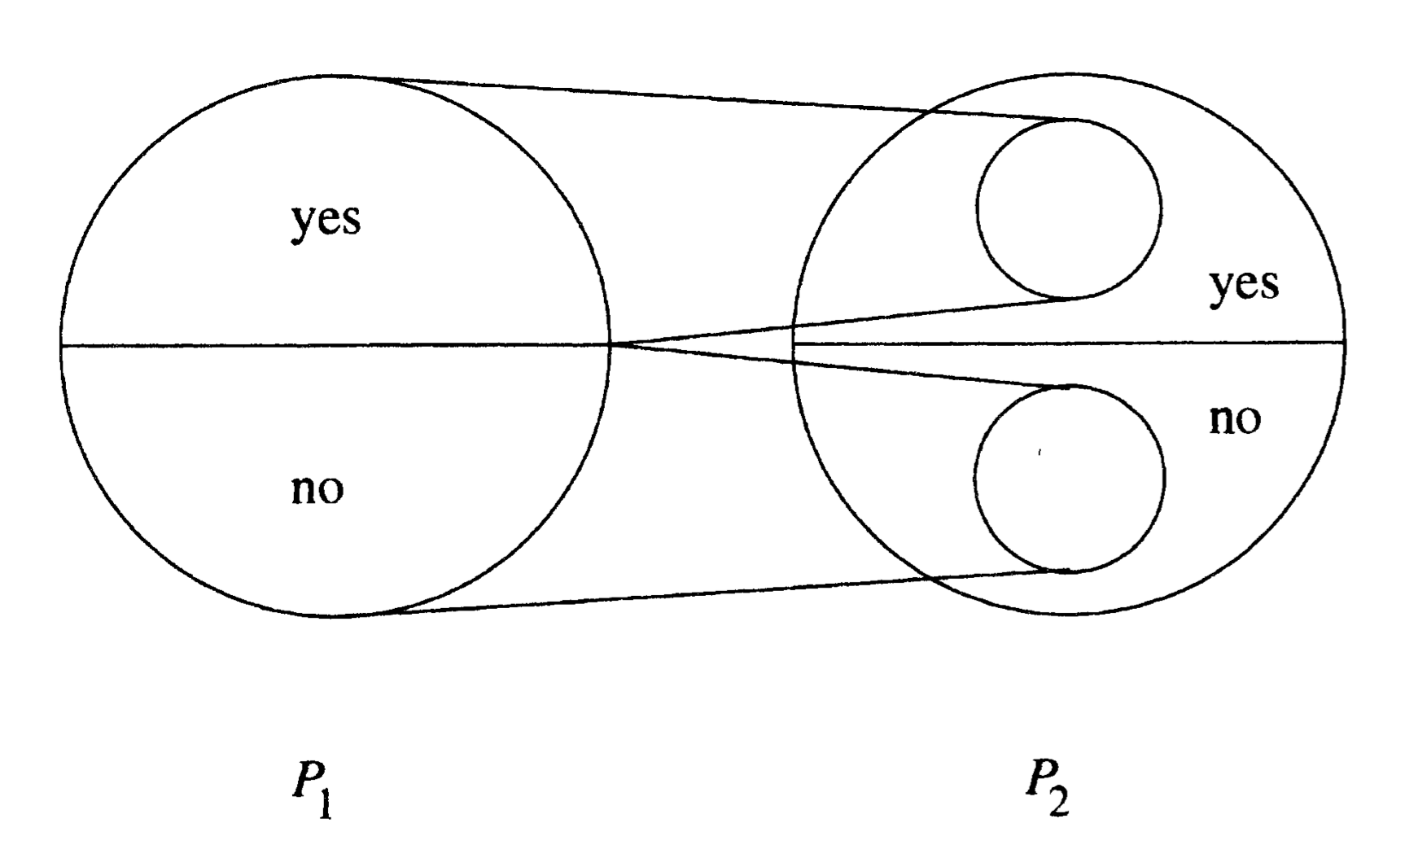
\includegraphics[width=0.4\textwidth]{reduction}
\end{figure}
\begin{theorem}[Reductions]
  Suppose $P_1\le _m P_2$. Then
  \begin{enumerate}
    \item If $P_1$ is not recursive, $P_2$ is not recursive.
    \item If $P_1$ is not RE, $P_2$ is not RE.
    \item If $P_2$ is recursive, $P_1$ is recursive.
    \item If $P_2$ is RE, $P_1$ is RE.
  \end{enumerate}
\end{theorem}

To show that a problem $P$ is hard, we pick a problem $P'$ which is hard and
then show that $P'\le _m P$, by constructing a recursive function $f$ such that
$x\in P'\iff f(x)\in P$.

\begin{example}[TMs with an Nonempty Language]
  The set of encoded TMs with at least one string, $L_{ne}=\left\{ M|L\left( M
  \right) \neq \emptyset  \right\} $ is RE but not recursive.
\end{example}
\begin{proof}
  Consider a TM $M'$, such that:
  \begin{lstlisting}[mathescape]
  M'$(M)$:
    for $t=0$ to $\infty$:
      for $i=0$ to $t$:
        if M$(\omega_i)$ accepts within $t$ steps, M' accepts.
      endfor
    endfor
  endM'
  \end{lstlisting}
  The algorithm tries $\omega_1$ with $1$ step, then $\omega_1, \omega_2$ with
  $2$ steps, and so on. If $M$ accepts any string in the alphabet, it will halt
  and accept. Hence $L(M)=L_{ne}$ and $L_{ne}$ is RE.\\

  To show that $L_{ne}$ is not recursive, we consider the complement of
  $L_{ne}$, $L_e=\left\{ M|L(M)=\emptyset  \right\} $, and show that
  $\bar{L_U}\le _m L_e$, and hence $L_e$ is not RE. We want to find a recursive
  function that finds a TM $M'$ such that 
  \[L(M')=\emptyset \iff \omega\not\in L(M).\]
  Given input $\left( M,\omega \right) $, we define
  \begin{lstlisting}[mathescape]
  M'($x$):
    for $t=0$ to $\infty$:
      if M$(\omega)$ accepts within $t$ steps, M' accepts.
    endfor
  endM'
  \end{lstlisting}
  If $M$ accepts $\omega$, $M'$ accepts all strings and $L(M')\neq \emptyset $.
  If $M$ does not accept $\omega$, $M'$ does not accept any output.
  Since $\bar{L_U}$ is not RE, $L_{e}$ is not RE.\\

  $L_{ne}$ is RE but $L_e$ is not RE, hence they are not recursive.
\end{proof}


\subsubsection{Properties of RE Languages}
\begin{definition}[Properties]
  A \textit{property} of the RE languages is a subset of the $RE$ languages.
\end{definition}
\begin{definition}[Trivial Properties]
  A \textit{trivial property} is a property that is either empty or all RE
  languages. A property is nontrivial $\iff$ there exists a language that
  fulfils a property and a language that doesn't.
\end{definition}
\begin{definition}[Semantic Properties]
  A property $P$ is semantic if it pertains only the behaviour of the program,
  rather than its syntax. 
  \[L_1=L_2\implies L_1\in P\iff L_2\in P\]
\end{definition}

\begin{theorem}[Rice Theorem]
  All nontrivial semantic properties of the RE languages is undecideable.
\end{theorem}
\begin{proof}
  Suppose $\mathcal{P}$ a nontrivial property of RE languages. We show that
  $L_e\le L_\mathcal{P}$. That is, there exists a recursive function $f$ such
  that
  \[M\in L_e\iff f(M)\in L_\mathcal{P}.\]
  WLOG, assume $\emptyset $ satisfies $\mathcal{P}$ (otherwise, consider
  $\bar{\mathcal{P}}$). Let $L$ be a RE language that does not satisfy
  $\mathcal{P}$, and $M''$ the machine that accepts $L$. Given a TM $M$,
  we define $M'$:
  \begin{lstlisting}[mathescape]
M'$(x)$:
  for $t=0$ to $\infty$:
    for $i=0$ to $t$:
      if M$(\omega_i)$ accepts within $t$ steps $\wedge$ M''$(x)$ accepts within $t$ steps, M' accepts $x$. 
    endfor
  endfor
endM'
  \end{lstlisting}
  If $L(M)=\emptyset $, $L(M')=\emptyset $ that satisfies $\mathcal{P}$. If
  $L(M)\neq\emptyset $, $L(M')=L$ that does not satisfy $\mathcal{P}$. Since
  $L_e$ is not recursive, $L_\mathcal{P}$ is not recursive.
\end{proof}

\begin{remark}
  Rice's theorem does not imply that everything about a TM is undecidable. For
  instance, syntactic properties, such as the number of states of the TM, is
  decidable.
\end{remark}

\subsection{Undecidable Problems}
With the groundwork of undecidability and TMs laid out, we may move on to prove
the undecidability of problems involving beyond TMs and their languages. We
begin with the Post's Correspondence Problem, which involves strings rather
than TMs.

\subsubsection{Post's Correspondence Problem}
PCP consists two lists of strings, of equal length $k\in \mathbb{N}$, over an
alphabet $\Sigma$.
\[A=w_1,w_2,\ldots,w_k \qquad B=x_1,x_2,\ldots,x_k\]
Each $i\in \mathbb{N}_{\le k}$ specifies a \textit{corresponding pair} $\left(
w_i,x_i \right) $. A solution to PCP is a nontrivial sequence of integers
$i_1,i_2,\ldots,i_m$ taken as indices of corresponding pairs, that yield the
same string when concatenated.
\[w_{i_1}w_{i_2}\cdots w_{i_m}=x_{i_1}x_{i_2}\cdots x_{i_m}.\]
PCP is the decision problem for the existence of a solution.

\paragraph{``Modified'' PCP} To prove the undecidability of PCP, we first
consider a modified problem as an intermediate reduction. We define MPCP to be
an instance of PCP, with the additional constraint that the first corresponding
pair must also be the first pair in the solution. A solution similarly
comprises a sequence of integers $i_1,i_2,\ldots,i_m$ such that
\[w_1w_{i_1}w_{i_2}\cdots w_{i_m}=x_1x_{i_1}x_{i_2}\cdots x_{i_m}.\]

\begin{prop}
  MPCP is reducible to PCP.
\end{prop}
Suppose an instance of MPCP with lists $A=w_1,w_2,\ldots,w_k$ and
$B=x_1,x_2,\ldots,x_k$. WLOG, assume $*,\$\not\in\Sigma$. We construct a PCP
instance with $C=y_0,y_1,\ldots,y_{k+1}$ and $D=z_0,z_1,\ldots,z_{k+1}$ where:
\begin{itemize}
  \item For $i=1,2,\ldots,k$, $y_i:=w_i\cdot *$ and $z_i:=*\cdot x_i$
  \item $y_0:= *\cdot y_1$ and $z_0:=z_1$
  \item $y_{k+1}:=\$$ and $z_{k+1}:=*\$$
\end{itemize}
\begin{proof}
  ($\implies$) Suppose $i_1,i_2,\ldots,i_m$ is a solution to the MPCP instance.
  \[w_1w_{i_1}w_{i_2}\cdots w_{i_m}=x_1x_{i_1}x_{i_2}\cdots x_{i_m}.\]
  Applying the defined transformations, we have the equal strings
  \[*\cdot y_1y_{i_1}y_{i_2}\cdots y_{i_m}=z_1z_{i_1}z_{i_2}\cdots z_{i_m}\cdot *.\]
  Since $y_0=*\cdot y_1$, $z_0=z_1$, and $y_{k+1}=\$$, $z_{k+1}=*\$$, we have
  \[y_0y_{i_1}y_{i_2}\cdots y_{i_m}y_{k+1}=z_0z_{i_1}z_{i_2}\cdots z_{i_m} z_{k+1}\]
  and $0,i_1,i_2,\ldots i_m,k+1$ is a solution to the PCP instance.\\

  ($\impliedby$) Suppose a solution to the PCP instance. It must begin with
  index $0$ and end with index $k+1$ since they are the only corresponding
  pairs with the same start symbol and end symbol, respectively.
  \[y_0y_{i_1}y_{i_2}\cdots y_{i_m}y_{k+1}=z_0z_{i_1}z_{i_2}\cdots z_{i_m} z_{k+1}\]
  Removing the $*$s and the final $\$$, we have
  \[w_1w_{i_1}w_{i_2}\cdots w_{i_m}=x_1x_{i_1}x_{i_2}\cdots x_{i_m}\]
  and $1,i_1,i_2,\ldots,i_m$ is a solution to the MPCP instance.\qed
\end{proof}

\begin{prop}
  $L_U$ is reducible to MPCP.
\end{prop}
Suppose a pair $\left( M,\omega \right)$. WLOG, assume the TM never writes a
blank and the tape is semi-infinite (to the right). Each ID is hence of the
form $\alpha q\beta$ where $\alpha\in \Gamma^{+}, q\in Q, \beta\in \Gamma^{*}$.
For $M=\left( Q,\Sigma,\Gamma,\delta,q_0,B,F \right) $, we define the following
pairs in our MPCP instance
\begin{enumerate}
  \item $w_1=\#$ and $x_1=\#q_0w\#$ which must start the solution of MPCP to
    begin the simulation of $M$. 
  \item $w_2=x_2=\#$. For each $X\in \Gamma$, $w_i=x_i=X$.
  \item For all $q\in Q-F$, $p\in Q$, $X,Y,Z\in \Gamma$, 
    \begin{itemize}
      \item $w_i=qX$, $x_i=Yp$ if $\delta\left( q,X \right) =\left( p,Y,R \right) $
      \item $w_i=ZqX$, $x_i=pZY$ if $\delta\left( q,X \right) =\left( p,Y,L \right) $
      \item $w_i=q\#$, $x_i=Yp\#$ if $\delta\left( q,B \right) =\left( p,Y,R \right) $
      \item $w_i=Zq\#$, $x_i=pZY\#$ if $\delta\left( q,B \right) =\left( p,Y,L \right) $
    \end{itemize}
    Each of these pairs extend the $B$ string to add the next ID and extend the $A$ string
    to match the $B$ string.
  \item For all $q\in F$, $X,Y\in \Gamma$
    \begin{itemize}
      \item $w_i=XqY$, $x_i=q$
      \item $w_i=Xq$, $x_i=q$
      \item $w_i=qY$, $x_i=q$
    \end{itemize}
    These pairs allow us to consume all tape symbols after achieving an
    accepting state. This allows us to simplify to match the final step.
  \item $w_i=q\#\#$, $x_i=\#$. When the tape is emptied, we may use the final
    pair to complete the solution.
\end{enumerate}

Intuitively, the MPCP simulates the computation of $M$ on $\omega$, each
partial solution consisting strings that are prefixes of the sequence of IDs of
$M$, $\#\alpha_1\#\alpha_2\#\alpha_3\#\cdots$. The string from $B$ is one ID
ahead of that from $A$, unless $M$ enters an accepting state, where it would be
able to ``catch up'' to obtain a solution. Then $M$ accepts $\omega$ $\iff$
there is a solution to this instance of MPCP.\\

Since $L_U\le _m MPCP \le _m PCP$, by transitivity, since $L_U$ is undecidable,
PCP is undecidable.
\begin{theorem}
  PCP is undecidable.
\end{theorem}

\subsubsection{Ambiguous Grammars}
Using PCP, we may further prove the undecidability of other problems, particularly
that the ambiguity of a grammar is undecidable. Suppose an instance of PCP with lists
$A=w_1,w_2,\ldots,w_k$ and $B=x_1,x_2,\ldots,x_k$. WLOG, suppose
$a_1,a_2,\ldots,a_k\not\in \Sigma$. Consider the grammar, for $i\in \left[ 1,k
\right] $
\begin{gather*}
  S\to A|B\\
  A\to w_iAa_i| w_ia_i\\
  B\to x_iBa_i| x_ia_i
\end{gather*}
The grammar is ambiguous $\iff L(G_A)\cap L(G_B)\neq \emptyset \iff$ The
instance of PCP has a solution, where $G_A$ is the grammar of productions
involving $A$ and that of $B$ for $G_B$.

\begin{remark}
  $\bar{L\left( G_A \right) },\bar{L\left( G_B \right) }$ are CFLs.
\end{remark}

Using the undecidability of the intersection of $L(G_A)$ and $L(G_B)$, we may
prove the undecidability of various other decision problems.
\begin{example}[$L(G_1)=L(G_2)$]
  Take $L(G_1)=\bar{L(G_A)}\cup \bar{L(G_B)}=\bar{L(G_A)\cap L(G_B)}$ and
  $L(G_2)={\left( \Sigma\cup \left\{ a_1,a_2,\ldots \right\}  \right)}^{*}$.
\end{example}

\subsection{Unrestricted Grammars}
\begin{definition}[Unrestricted Grammar]
  A UG $G=\left( N,\Sigma,S,P \right) $, where:
  \begin{itemize}
    \item $N$: A finite set of non-terminals
    \item $\Sigma$: A finite set of terminals, $N \cap \Sigma=\emptyset $
    \item $S$: A start symbol, $S\in V$ 
    \item $P$: A finite set of productions
  \end{itemize}
  A production, contrary to CFGs, is of the form $\alpha\to\beta$, where
  $\alpha\in {\left( N \cup \Sigma \right)}^{*}N{\left( N\cup \Sigma
  \right)}^{*}$ and $\beta\in {\left( N \cup \Sigma \right)}^{*}$.
\end{definition}

\begin{theorem}
  The languages generated by unrestricted grammars are exactly the languages
  generated by TMs.
\end{theorem}

\begin{definition}[Context Sensitive Grammar]
  A CSG is a UG with the additional constraint that $\left| \alpha \right| \le
  \left| \beta \right| $.
\end{definition}
\begin{definition}[Context Sensitive Languages]
  If $L$ is $L(G)$ for some CSG $G$, then $L$ is a \textit{context-sensitive language}.
\end{definition}
\begin{example}[$\left\{ a^{n}b^{n}c^{n}|n\in \mathbb{N}^{*} \right\}$]
   \begin{gather*}
     S\to aSBC|aBC\\
     CB\to BC\\
     aB\to ab\\
     bB\to bb\\
     bC\to bc\\
     cC\to cc
   \end{gather*}
\end{example}

\begin{remark}
  The class of context sensitive languages are exactly $NSPACE\left( O\left( n
  \right)  \right) $. They are closed under intersection, union and concatenation.
\end{remark}

\section{Complexities and Classes}
Within the recursive class of languages accepted by TMs and hence our
computers, we consider the time and space complexities of their computations.
We so define on an TMs with multiple, but fixed, number of tapes, with finite
tape alphabets. This allows us to divide the class into the \textit{tractable}
and the \textit{intractable} problems.

\subsubsection{Complexity Measures}
In measuring the complexity of a program, we want to find a function $\Phi:
\mathbb{N}\times \mathbb{N}\to \mathbb{N}$ that measures the ``complexity'', or
cost of a TM on some input. We denote $\Phi\left( i,x \right)=\Phi_i\left( x
\right)$ for the complexity of TM $M_i$ with the input $x$. We hence have the
first of Blum's complexity axioms:
\[Dom\left( \phi_i \right)=Dom\left( \Phi_i \right).\]
where $\phi$ is the $i$-th program/TM.  Further, the complexity measure should
be computable for practicality. We have the second of Blum's complexity axioms:
\[\text{The set }\left\{ i,x,B  \in \mathbb{N}^{3}|\Phi_i\left( x \right)
<B\right\}\text{ is recursive}.\]

\begin{definition}[Blum Complexity Measure]
  A \textit{Blum complexity measure} $\iff$ $\Phi\left( i,x \right) $ is a
  partial recursive function that satisfies the two Blum's complexity axioms.
\end{definition}

\subsubsection{Time/Space Complexity Measures}

\begin{definition}[Running Time]
  The \textit{running time} of a TM $M$ on input $\omega$, $Time_M\left(
  \omega \right)$, is the number of steps made by $M$ before halting. If $M$
  does not halt on input $x$, $Time_M\left( x \right) =\infty$.
\end{definition}

\begin{definition}[Time Complexity]
  The \textit{time complexity} of a TM $M$ is the function $T(n)$ that is
  the maximum of the running time of $M$ on  all inputs $\omega$
  of length $n$.
  \begin{center}
    $M$ is $T(n)$ time bounded $\iff\forall$ inputs $\omega$ of length $n$,
    $Time_M\left( \omega \right) \le T(n)$
  \end{center}
\end{definition}

We may further define its analogues for space.
\begin{definition}[Space Consumption]
  The \textit{space consumption} of a TM $M$ on input $\omega$, $Space_M\left(
  \omega \right) $, is the maximum number of cells ``touched'' by $M$ on any of
  its worktapes before halting. If $M$ does not halt on an input $x$,
  $Space_M\left( x \right) =\infty$.
\end{definition}

\begin{definition}[Space Complexity]
  The \textit{space complexity} of a TM $M$ is the function $S(n)$ that is
  the maximum of the space consumption of $M$ on all inputs $\omega$
  of length $n$.
  \begin{center}
    $M$ is $S(n)$ space bounded $\iff\forall$ inputs $\omega$ of length $n$,
    $Space_M\left( \omega \right) \le S(n)$
  \end{center}
\end{definition}

\begin{prop}[Existence of Arbitrary Difficult Problems]
  Suppose a recursive function $f$. We define
  \begin{lstlisting}[mathescape]
  g$\left( x \right)$:
    Simulate $M_x$ on input $x$.
    if $M_x$ does not halt within $f\left(\left|x\right|\right)$ steps, output $0$.
    else output $M_x(x)+1$. // or anything not $M_x(x)$
  endg
  \end{lstlisting}
  $g$ cannot be computed by any $f(n)$ time bound TM.
\end{prop}
\begin{proof}
  Suppose not. Consider the $f(n) $ time bound TM $M_y$ that computes $g$.
  Consider $M_y\left( y \right)$. $M_y$ must halt within $f(\left| y \right|)$
  steps since it is $f(n)$ time bound. Hence $M_y\left( y \right) $ outputs
  $M_y(y)+1$. A contradiction.\qed
\end{proof}

\begin{definition}[Space Constructible Functions]
  A function $S(n)$ is \textit{fully space constructible} if there exists a
  $S(n)$ space bounded TM $M$ such that on all inputs of length $n$, it uses
  space exactly $S(n)$.
\end{definition}

\begin{definition}[Time Constructible Functions]
  A function $T(n)$ is \textit{fully time constructible} if there exists a
  $T(n)$ time bounded TM $M$ such that on all inputs of length $n$, it halts
  and uses time exactly $T(n)$.
\end{definition}

\subsection{Definitions}
\begin{definition}[P]
  A language $L$ is in the class \textit{P} if there exists a
  \textbf{deterministic} TM $M$ and a polynomial time complexity $T(n)$ such
  that $L=L(M)$ and $M$ is $T(n)$ time bounded.
\end{definition}

\begin{definition}[NP]
  A language $L$ is in the class \textit{NP} if there exists a
  \textbf{nondeterministic} TM $M$ and a polynomial time complexity $T(n)$ such
  that $L=L(M)$ and $M$ is $T(n)$ time bounded.
\end{definition}

\begin{definition}[co-NP]
  A language $L$ is in the class \textit{co-NP} if its complement $\bar{L}$ is
  in NP.
\end{definition}

\begin{definition}[Certificate]
  A \textit{certificate} (witness) is a string that certifies the answer to a
  computation, or membership of some string in a language. Intuitively, a
  certificate is the ``answer'' to the problem at hand.
\end{definition}
\begin{prop}
  $L$ is in NP $\iff$ there exists a polynomial $q\left( \cdot \right) $ and a
  polynomial-time bounded TM $M$ such that 
  \[x\in L \iff \exists \text{ a certificate } c, \left| c \right| \le
  q\left(\left| x \right| \right) \text{$M$ accepts the pair $\left( x,c
\right) $}.\]
  That is, we can verify a solution of the problem in polynomial time.
\end{prop}

\subsection{NP-Completeness}
\begin{definition}[NP Hard]
  A language (problem) $L$ is \textit{NP hard} if for every language $L'\in
  NP$ there is a polynomial time reduction of $L'$ to $L$.
\end{definition}

\begin{definition}[NP Complete]
  A language (problem) $L$ is \textit{NP complete} if $L$ is in NP, and it is
  NP hard. That is, for every language $L'\in NP$ there is a polynomial time
  reduction of $L'$ to $L$.
\end{definition}

\begin{definition}[Karp Reducibility]
  A problem $P_1$ is \textit{Karp reducible} to $P_2$, $P_1\le _m^{p} P_2$, if
  there exists a polynomial time computable recursive function $f$ such that
  \[x\in P_1\iff f(x)\in P_2.\]
  We say that $P_1$ is polynomial time, many-one reducible to $P_2$.
\end{definition}

\begin{remark}
  We may further define an alternative notion of reducibility known as a
  \textit{Cook reducibility}.  A problem $P_1$ is \textit{Cook reducible} to
  $P_2$, $P_1\le _T^{p} P_2$, if, given an oracle for $P_2$, there exists a
  polynomial time recursive algorithm that solves $P_1$. This presents another
  type of NP-completeness known as Cook-completeness. In the course and in many
  conventions, we use the more retricted notion of Karp-completeness.
\end{remark}

Since the reducible relation is reflexive and transitive, it is sufficient to
prove that if $L$ is NP complete, $L'\in NP$, $L\le^{p}_m L'$, then $L'$ is NP
complete. We can hence prove the NP-completeness of some problem $P$ with a
known NP-complete problem $P'$ that Karp-reduces to $P$ and that $P$ is NP.

\begin{theorem}
  If  one of the NP complete problems is solvable in polynomial time, all the
  problems in NP are solvable in polynomial time. That is, $P=NP$.
\end{theorem}

\subsection{Known NP-Complete Problems}
\subsubsection{Satisfiability} Suppose a set $U$ of variables and a collection $C$
of clauses over $U$. Does there exist a satisfying truth assignment for $C$?
\begin{example}[Instance of Satisfiability]
  Let $U=\left\{ A,B,C,D,E,F \right\} $ be a set of variables. Consider
  the expression
  \[\left( A\vee B \vee \neg C\vee E\right)\wedge \left( E\vee F\vee \neg A
  \right) \left( C\vee F \right) \wedge \ldots.\]
  Is there a truth assignment to the literals such that the expression is true?
\end{example}
The 3-SAT problem is the Satisfiability problem, with each clause containing
exactly 3 literals.

\subsubsection{3-Dimensional Matching} Suppose $3$ disjoint finite sets $X,Y,Z$ of
equal cardinality $n$,  and a set $S\subseteq X\times Y\times Z $. Does $S$
contain a matching (a subset $S'\subseteq S$ of cardinality $n$ such that for
any two distinct $\left( x_1,y_1,z_1 \right) , \left( x_2,y_2,z_2 \right) \in
S'$, $x_1\neq x_2$, $y_1\neq y_2$, and $z_1\neq z_2$)?\\

\subsubsection{Vertex Cover} Suppose a graph $G=\left( V,E \right) $ and a
positive integer $K\le \left| V \right| $. Is there a vertex cover $V'$ of size
$\le K$?\\

\begin{proof}
  Given a graph $\left( V,E \right) $, guess a $V'\subseteq V$ and verify if
  $\left| V' \right| \le k$ and $\forall \left( v,w \right) \in E$, at least
  one of $v,w$ is in $V'$. Vertex Cover is in NP.\\

  Suppose an instance of 3SAT, with the set of variables $U=\left\{
  x_1,x_2,\ldots,x_{n} \right\} $, the set of clauses $C=\left\{
c_1,c_2,\ldots,c_m \right\} $ where $c_i=\left( l_{i,1}\vee l_{i,2}\vee l_{i,3}
\right) $.

  Consider a vertex cover instance $G=\left( V,E \right) $, where:
  \begin{gather*}
    V=\left\{ u_i,w_i|1\le i\le n \right\} \cup \left\{ z_{j,1},z_{j,2},z_{j,3}
    | 1\le j\le m\right\} \\
    E=\left\{ \left( u_i,w_i \right) | 1\le i\le n \right\} \cup \left\{ \left(
    z_{j,1}, z_{j,2} \right), \left( z_{j,1}, z_{j,3} \right), \left( z_{j,2},
z_{j,3} \right) | 1\le j\le m \right\}\cup \left\{ \left( z_{j,r}, u_i \right)
| l_{j,r}=x_i \right\} \cup \left\{ \left( z_{j,r}, w_i \right) | l_{j,r}=\neg
x_i \right\}\\
  K=2m+n
  \end{gather*}
  Each $u_i$ represents $x_i$, $w_i$ represents $\neq x_i$, and $z_{j,r}$
  represents the $l_{j,r}$. This reduction can be done in polynomial time. We
  want to show that the 3SAT instance has a solution $\iff$ the vertex cover
  instance has a solution.\\

  In a vertex cover, 
  \begin{itemize}
    \item For each $1\le i\le n$, at least one of $u_i, w_i$ is in the cover.
      (A pair representing a variable and its complement)
    \item For each $1\le j\le m$, at least two of $z_{j,1},z_{j,2},z_{j,3}$ is
      in the cover. (A triangle representing each clause)
  \end{itemize}
  Since we have the size bound $K=2m+n$, \textit{exactly} one and two
  (respectively) of the vertices are in the cover.\\

  ($\implies$) Suppose the 3SAT instance is satisfiable. By choosing $u_i$
  $\iff$ $x_i$ is true and $x_i$ $\iff$ $x_i$ is false, and choosing two of
  $z_{j,a}$ such that the one left out represents the true literal, we have a
  vertex cover of $G$.

  ($\impliedby$) Suppose the vertex cover instance has a solution. Consider the
  truth assignment such that $x_i$ is true $\iff$ $u_i$ is in the vertex cover.
  It can be shown that if $z_{j,r}$ is not in the vertex cover then $l_{j,r}$
  must be true.\\

  Hence Vertex Cover is NP Complete.\qed
\end{proof}

\subsubsection{MAX-CUT} Suppose an undirected graph $G=\left( V,E \right) $ and a
positive integer $K\le \left| E \right| $. Does there exist a cut of $G$ with
size $>K$? 

\subsubsection{Clique} Suppose a graph $G=\left( V,E \right) $ and a positive
integer $K\le \left| V \right| $. Does $G$ contain a clique of size $\ge K$ (a
subset larger than $K$ of $V$ that can form a complete graph with edges in
$E$)?

\subsubsection{Independent Set} Suppose a graph $G=\left( V,E \right) $ and a
positive integer $K\le \left| V \right| $. Does $G$ contain an independent set
of size $\ge K$ (a subset larger than $K$ of $V$ such that no distinct pair of
vertices are adjacent)?\\

\begin{proof}
  Given a graph $\left( V,E \right) $, guess a $V'\subseteq V$ and verify if
  $\left| V' \right| \le K$ and that it is a complete graph. Clique is in NP.
  Similarly for Independent Set.\\

  Suppose $G=\left( V,E \right) $. $V'$ is a vertex cover of $G$ $\iff$ $V-V'$
  is an independent set of $G$ $\iff$ $V-V'$ is a clique of $G'$, where $G'$ is
  the complement of $G$. That is, the graph has a vertex cover of size $k$
  $\iff$ $G$ has an independent set of size $\left| V \right| -k$ $\iff$ $G'$
  has a clique of size $\left| V \right| -k$.\\

  Hence Clique/Independent Set is NP Complete.\qed
\end{proof}

\subsubsection{Hamiltonian Circuit} Suppose a graph $G=\left( V,E \right) $. Does
$G$ contain a Hamiltonian circuit (a simple circuit that goes through all
vertices of $G$)?

\subsubsection{Partition} Suppose a finite set $A$ and a size function $s: A\to
\mathbb{R}^{*}_{+}$. Is there a subset $A'\subseteq A$ such that
\[\sum_{a\in A'}s(a)=\sum_{a\in A-A'}s(a)?\]

\subsubsection{Set Cover} Suppose a finite set $A$, a collection of sets from $A$
$\left\{ S_1,S_2,\ldots,S_m \right\} \subseteq \mathcal{P}\left( A \right) $,
and $k\in \mathbb{N}$. Does there exist a subset $Y\subseteq \left\{
1,2,\ldots,m \right\} $, $\left| Y \right| \le k$ such that
\[A\subseteq  \bigcup_{i \in Y} S_i?\]

\subsubsection{Travelling Salesman Problem} Suppose a complete weighted graph
$G=\left( V,E \right) $, and a bound $B\in \mathbb{R}^{*}_{+}$. Is there a
hamiltonian circuit of total weight $\le B$?

\subsection{Modifications to TMs}
\begin{theorem}[Tape Compression]
  Suppose a constant $c\in \mathbb{R}^{*}_{+}$. If a language $L$ is accepted
  by a $S(n)$ space bounded TM $M$ with $k$ tapes, there exists a TM $M'$ with
  $k$ tapes that is $\lceil cS(n)\rceil$ space bounded that accepts $L$.
\end{theorem}
\begin{proof}
  Suppose a TM $M$ that is $S(n)$ space bounded and accepts a language $L$.\\

  Consider the TM $M'$, where each cell of a worktape of $M'$ encodes $m$ cells
  of the corresponding tape of $M$. Then the tape alphabet
  $\Gamma_{M'}={\Gamma_M}^{m}$. Through variable storage in the finite control
  of $M'$, we keep track of which of the $m$ cells is the currently scanned
  cell. Hence $M'$ is able to simulate $M$, and accepts $\iff$ $M$ accepts.\\

  The space used by $M'$ on input $x$ is:
  \[\lceil \frac{Space_M\left( x \right) }{m}\rceil.\]
  Taking $m>\frac{1}{c}$, $M'$ is $\lceil cS(n) \rceil$ space bounded.\qed
\end{proof}

\begin{theorem}[Linear Speedup]
  Suppose a constant $c\in \mathbb{R}^{*}_{+}$. Suppose a language $L$ is accepted
  by a $T(n)$ time bounded TM $M$ with $k\ge 2$ tapes, where
  \[\lim_{n \to \infty} \frac{T(n)}{n}=\infty.\]
  Then there exists a TM $M'$ with $k$ tapes that is $\lceil cT(n)\rceil$ time
  bounded that accepts $L$.
\end{theorem}

\begin{corollary}[Linear Speedup]
  Suppose a constant $c\in \mathbb{R}^{*}_{+}$. Suppose a language $L$ is accepted
  by a $T(n)$ time bounded TM $M$ with $k\ge 2$ tapes, where
  \[T(n)=dn,\qquad d\in \mathbb{R}^{*}_+.\]
  Then there exists a TM $M'$ with $k$ tapes that is $\left( 1+c \right) n$
  time bounded that accepts $L$.
\end{corollary}

\subsection{Complexity Classes}
\begin{notation}[Time and Space Complexity Classes]
  \begin{gather*}
    DSPACE(S(n))=\left\{ L|\exists \text{ DTM }M, L(M)=L\wedge M\text{ is
    }S(n)\text{ space bounded.} \right\} \\
    DTIME(T(n))=\left\{ L|\exists \text{ DTM }M, L(M)=L\wedge M\text{ is
    }T(n)\text{ time bounded.} \right\} \\
    NSPACE(S(n))=\left\{ L|\exists \text{ NTM }M, L(M)=L\wedge M\text{ is
    }S(n)\text{ space bounded.} \right\} \\
    NTIME(T(n))=\left\{ L|\exists \text{ NTM }M, L(M)=L\wedge M\text{ is
    }T(n)\text{ time bounded.} \right\} 
  \end{gather*}
\end{notation}

\begin{theorem}[Relationships between Complexity Classes]
  \begin{gather*}
    DTIME\left( S\left( n \right)  \right) \subseteq DSPACE\left( S\left( n
    \right)  \right) \\
    \text{If }L\in DSPACE\left( S\left( n \right)  \right)\text{ and }S\left(
    n \right) \ge\log{n}\text{, then there exists a constant }c(L)\in
    \mathbb{R_+^{*}}, L\in DTIME\left( c^{S\left( n \right) } \right)\\
    \text{If }L \in NTIME\left( T\left( n \right) \right)\text{, then there
    exists a constant } c(L)\in \mathbb{R}^{*}_+, L\in DTIME\left( c^{T\left( n
    \right) } \right) 
  \end{gather*}
\end{theorem}

\begin{theorem}[Savitch's Theorem]
  If $S(n)\ge \log{n}$, and $S\left( n \right) $ is fully space constructible, then
  \[NSPACE\left( S\left( n \right)  \right) \subseteq DSPACE\left( {\left( S\left( n \right)  \right) }^{2} \right).\] 
\end{theorem}

\begin{theorem}
  The class of languages that can be accepted in polynomial space by a DTM
  $PSPACE$ is equal to the class of languages that can be accepted in
  polynomial space by a NTM $NPSPACE$. $PSPACE=NPSPACE$
\end{theorem}

\subsubsection{Hierachy Theorems}
\begin{theorem}
  If $L$ is accepted by a $S(n)\ge \log{n}$ space bounded TM, then $L$ can be
  accepted by a $S(n)$ space bounded machine which halts on all inputs.
\end{theorem}
Hence, WLOG, we may assume that a TM with a large enough space bound halts on
all inputs.
\begin{theorem}[Space Hierachy]
  Suppose $S_2(n),S_1(n)\ge \log{n}$. If $S_2(n)$ is fully space constructible and
  \[\lim_{n \to \infty} \frac{S_1(n)}{S_2(n)}=0,\] 
  there is a language in $DSPACE\left( S_2\left( n \right)  \right)
  -DSPACE\left( S_1\left( n \right)  \right) $.
\end{theorem}
\begin{proof}
  Consider the TM $M$ which is $S_2\left( n \right) $ space bounded, with a
  fixed number of tapes.
  \begin{lstlisting}[mathescape]
  M$\left(x\right)$:
    if $x$ is of the form $1^k$, reject.
    Mark out space $S_2\left(\left|1^{k}0x\right|\right)$ on the work tape.
    Simulate machine $M_x$ on input $1^{k}0x$.
    if $M_x$ attempts to use more than $S_2\left(\left|1^k 0x\right|\right)$, $M$ rejects.
    if $M_x$ halts and rejects the input, $M$ accepts.
  endM
  \end{lstlisting}
  Let $L=L(M)$. Since $M$ is $S_2(n)$ space bounded, $L\in DSPACE\left(
  S_2\left( n \right)  \right) $.\\

  Suppose by way of contradiction that some TM $M'$ is $S_1(n)$ space bounded
  accepting $L$. There exists another $2$-tape machine $M_x$ accepting $L$
  using space $\le dS_1(n)$ for some constant $d$. WLOG, assume $M_x$ halts on
  all inputs.\\

  Simulation of $M_x$ requires space $cS_1(n)$ for some constant $c$. Hence, let
  $k$ be large enough such that
  \[cS_1\left( \left| 1^{k}0x \right|  \right) <S_2\left( \left| 1^{k}0x
  \right|  \right).\]
  The simulation of $M_x$ must complete, and $M$ accepts $\iff$ $M_x$ did not.
  $M_x$ accepts a different language than $L$. A contradiction. \qed
\end{proof}

\begin{theorem}[Time Hierachy]
  Suppose $T_2(n),T_1(n)\ge \left( 1+\epsilon \right) {n}$. If $T_2(n)$ is
  fully time constructible and
  \[\lim_{n \to \infty} \frac{T_1(n)\log{\left( T_1\left( n \right)  \right) }}{T_2(n)}=0,\] 
  there is a language in $DTIME\left( T_2\left( n \right)  \right) -DTIME\left(
  T_1\left( n \right)  \right) $.
\end{theorem}
\begin{proof}
  Consider a machine $M$ with at least $5$ tapes (or more for fully time
  constructibility of $T_2\left( n \right) $). While running $M$, $M$ keeps
  track of the number of steps taken, and rejects if $T_2(n)$ time is exceeded.
  \begin{lstlisting}[mathescape]
  M$\left(x\right)$:
    if $x$ is of the form $1^k$, reject.
    Simulate $M_x$ on input $1^{k}0x$.
    if $M_x$ halts (does not exceed the time limit) and rejects the input, $M$ accepts.
  \end{lstlisting}
  Let $L=L(M)$. Since $M$ is $O(T_2(n))$ time bounded, $L \in DTIME\left(
  T_2(n) \right) $by linear speedup.

  Suppose by way of contradiction that some TM $M'$ is $T_1(n)$ time bounded
  accepting $L$. There exists another $2$-tape machine $M_x$ accepting $L$
  that is $dT_1(n)\log{T_1(n)}$ time bounded, for some constant $d$.\\

  Simulation of $M_x$ requires time $cT_1(n)\log{T_1(n)}$ for some constant
  $c$. Hence, let $k$ be large enough such that
  \[cT_1\left( \left| 1^{k}0x \right|  \right)\log{\left( T_1\left( \left|
  1^{k}0x \right|  \right)  \right) } <T_2\left( \left| 1^{k}0x \right|
\right).\]
  The simulation of $M_x$ must complete, and $M$ accepts $\iff$ $M_x$ did not.
  $M_x$ accepts a different language than $L$. A contradiction. \qed
\end{proof}

\end{document}
